% !TeX program = xelatex
% 论文逐句双语学习笔记；原文公式编号保留。
% 证明尽量沿用原文符号；M_n、S_n、T_n 按原文实际展开的区域详证，其余同理。
\documentclass[lang=cn,scheme=chinese,mode=simple,device=normal,color=blue,math=cm,thmcnt=chapter,bibend=bibtex,12pt]{elegantbook}
\newif\ifmathanalysiswatermark
\mathanalysiswatermarkfalse
% =============================================================================
% 可积系统 / Riemann--Hilbert 方法学习笔记：个人与项目级设置
%
% 设计原则：
% 1. 通用、稳定、适合所有 ElegantBook 文档的设置放进 elegantbook.cls；
% 2. 与个人习惯、当前项目或展示风格有关的设置放在本文件；
% 3. 以后想改页眉、水印文字、callout 样式、自定义命令，只改本文件即可。
% =============================================================================

% ================= 项目结构 =================
% subfiles 用于把大文档拆成多个可单独编译的子文件。
% 当前第五章虽然是独立编译，但保留这个宏包，便于以后扩展。
% ================= 子文件支持 ===============
\usepackage{subfiles}

% 单章编译可能读取 TeX Live 自带的 elegantbook.cls，故不使用文档类选项
% 控制水印，而统一读取主文件中定义的项目级开关。
\usepackage{draftwatermark}

% ================= 水印内容 =================
\SetWatermarkScale{0.4}
\SetWatermarkLightness{0.9}
\AtBeginDocument{%
    \ifmathanalysiswatermark
        \SetWatermarkText{欧拉的小迷弟}%
    \else
        \SetWatermarkText{}%
    \fi
}

% ================= 页眉页脚 =================
% 这是个人化设置，因此覆盖 ElegantBook 默认的 fancyhdr 样式。
%
% 左页眉：当前 section
% 右页眉：个人昵称
% 页脚中间：页码
\fancyhf{}
\fancyhead[L]{\rightmark}
\fancyhead[R]{欧拉的小迷弟}
\fancyfoot[C]{\thepage}
\renewcommand{\headrule}{\hrule width\headwidth}
\renewcommand{\headrulewidth}{0.4pt}
\pagestyle{fancy}

% chapter 首页默认使用 plain 页面样式。
% 这里重新定义 plain，使章首页也保持与普通页面相同的页眉页脚。
\fancypagestyle{plain}{%
    \fancyhf{}
    \fancyhead[L]{\rightmark}
    \fancyhead[R]{欧拉的小迷弟}
    \fancyfoot[C]{\thepage}
    \renewcommand{\headrule}{\hrule width\headwidth}
    \renewcommand{\headrulewidth}{0.4pt}%
}

% ================= 补充说明 callout 环境 =================
% ElegantBook 原生的 remark 环境保持不动。
%
% 本环境专门承载原 Obsidian 中的 callout，例如：
%
%   \begin{callout}[前置概念：Schwartz 空间]
%       ...
%   \end{callout}
%
% 设计目标：
% - 正文仍然是白底、正常字号；
% - callout 用浅灰背景 + 左侧竖线 + 小一号字体；
% - 组会汇报时可以快速区分“主线正文”和“补充材料”。
\newtcolorbox{callout}[1][]{
    enhanced,
    breakable,
    colback=black!3,
    colframe=black!35,
    boxrule=0pt,
    borderline west={1.4pt}{0pt}{black!45},
    arc=0pt,
    outer arc=0pt,
    left=8pt,
    right=8pt,
    top=7pt,
    bottom=7pt,
    before skip=10pt,
    after skip=10pt,
    title={#1},
    colbacktitle=black!7,
    coltitle=black,
    fonttitle=\bfseries\small,
    fontupper=\small,
    titlerule=0pt
}

% ================= 重要性标记 =================
% 用于在讲义中手动标记重点程度。
\newcommand{\marktriangle}{\ensuremath{\blacktriangle}}
\newcommand{\markstar}{\ensuremath{\bigstar}}
\newcommand{\markstartriangle}{\ensuremath{\bigstar\blacktriangle}}
\newcommand{\marktwostar}{\ensuremath{\bigstar\bigstar}}

% ================= 章节内部的小标题 =================
% 用于类似 (A)(B)(C)... 的无编号小标题。
%
% 当前定义会：
% 1. 显示为无编号 subsubsection；
% 2. 手动加入目录。
%
% 如果以后不希望这类小标题进入目录，只保留：
%   \subsubsection*{#1}
% 并删除 \addcontentsline 即可。
\newcommand{\methodsection}[1]{%
    \subsubsection*{#1}%
    \addcontentsline{toc}{subsubsection}{#1}%
}

% ================= 例题后的手写留白 =================
% 每道例题后统一空出 10 行正文高度，方便打印后手写。
% 若觉得太多或太少，只改这里的 10 即可。
\newcommand{\exampleblank}{\par\vspace{10\baselineskip}}

% 通用手动留白命令：\myspace{3} 表示空出 3 行正文高度。
\newcommand{\myspace}[1]{\par\vspace{#1\baselineskip}}

% ================= 自定义数学算子 =================
% 用 \DeclareMathOperator 定义后，排版时会使用直立字体和正确的运算符间距。
% 例如：$\rank A$、$\diag A$、$\Ker T$。
\DeclareMathOperator{\Tr}{Tr}
\DeclareMathOperator{\tr}{tr}
\DeclareMathOperator{\rank}{rank}
\DeclareMathOperator{\diag}{diag}
\DeclareMathOperator{\Ree}{Re}
\DeclareMathOperator{\Imm}{Im}
\DeclareMathOperator{\Ker}{Ker}
% ================= 行宽溢出容错 =================
\setlength{\emergencystretch}{2em}
% ================= enumerate 列表间距 =================
\setlist[enumerate]{
    itemsep=0.4em,
    topsep=0.5em,
    parsep=0pt,
    partopsep=0pt
}

% 本工程的局部设置；不修改父目录中的共享文档类和导言。
\hypersetup{hypertexnames=false,
  pdftitle={Hirota--Satsuma coupled KdV system：全文双语详解笔记},
  pdfauthor={学习笔记}}
\renewcommand{\proofname}{Proof／证明}
\renewcommand{\notename}{Note／注}
% 沿用当前 Windows 模板的楷体、仿宋；为其局部标题启用合成粗体，避免缺字形替代。
\IfFontExistsTF{KaiTi}{%
  \setCJKfamilyfont{hsnoteKai}[AutoFakeBold=2]{KaiTi}%
  \renewcommand{\citshape}{\CJKfamily{hsnoteKai}}}{}
\IfFontExistsTF{FangSong}{%
  \setCJKfamilyfont{hsnoteFangSong}[AutoFakeBold=2]{FangSong}%
  \renewcommand{\cfs}{\CJKfamily{hsnoteFangSong}}}{}
% 沿用 ElegantBook 的原生 thmstyle；独立计数以免触发本地自定义接口的空计数器问题。
\theoremstyle{thmstyle}
\newtheorem{paperlemmaen}{Lemma}[chapter]
\renewcommand{\thepaperlemmaen}{\thechapter.\arabic{paperlemmaen}}
% 中文陈述使用无编号环境，显示英文环境刚刚取得的同一个编号。
\newtheorem*{paperlemmacn*}{引理 \thepaperlemmaen}
\newtheorem{papertheoremen}{Theorem}[chapter]
\newtheorem*{papertheoremcn*}{定理 \thepapertheoremen}
\newtheorem{papercorollaryen}{Corollary}[chapter]
\newtheorem*{papercorollarycn*}{推论 \thepapercorollaryen}
\newtheorem{paperassumptionen}{Assumption}[chapter]
\newtheorem*{paperassumptioncn*}{假设 \thepaperassumptionen}
\theoremstyle{prostyle}
\newtheorem{paperpropositionen}{Proposition}[chapter]
\newtheorem*{paperpropositioncn*}{命题 \thepaperpropositionen}
\theoremstyle{defstyle}
\newtheorem{paperdefinitionen}{Definition}[chapter]
\newtheorem*{paperdefinitioncn*}{定义 \thepaperdefinitionen}
\newcommand{\EN}[1]{\par\noindent{\small\sffamily\color{black!50}EN}\enspace #1\par}
\newcommand{\CN}[1]{\par\noindent{\small\sffamily\color{black!50}中}\enspace #1\par}
\newcommand{\proofstep}[1]{\par\medskip\Needspace{3\baselineskip}\noindent\textbf{#1}\quad}
\newcommand{\originaleq}[1]{\tag{#1}\label{eq:#1}}
\newcounter{supplementeq}[chapter]
\newcommand{\supplementeq}[1]{\refstepcounter{supplementeq}\tag{S\thechapter.\arabic{supplementeq}}\label{#1}}
\newcommand{\dd}{\,\mathrm{d}}
\newcommand{\ii}{\mathrm{i}}
\newcommand{\Id}{I_4}
\newcommand{\Zero}{0_{2\times2}}
\newcommand{\OrigNine}{\hyperref[ref:original9]{[9]}}
\setlength{\jot}{5pt}
\setcounter{tocdepth}{2}
\setcounter{secnumdepth}{2}
\renewcommand{\thefigure}{\arabic{figure}}

\begin{document}
\frontmatter
\begin{titlepage}
\centering
\vspace*{2cm}
{\Large Riemann--Hilbert Approach for the\par}
\medskip
{\Large Hirota--Satsuma Coupled KdV System\par}
\vspace{1cm}
{\huge Hirota--Satsuma 耦合 KdV 系统\par}
\medskip
{\huge 的 Riemann--Hilbert 方法\par}
\vspace{1cm}
{\LARGE 逐句双语与完整推导学习笔记\par}
\vspace{0.6cm}
{\Large 全文逐句双语、校勘与推导\par}
\vfill
{\large 原文：Haibing Zhang、Xianguo Geng、Huan Liu\par}
\medskip
Studies in Applied Mathematics, 155 (2025), e70113\par
\href{https://doi.org/10.1111/sapm.70113}{DOI: 10.1111/sapm.70113}\par
\vspace{1cm}
2026 年 10 月 20 日\par
\end{titlepage}

\chapter*{阅读约定与必要背景}
\addcontentsline{toc}{chapter}{阅读约定与必要背景}
本笔记按论文的原章节顺序编排，保留原文的公式、定义、引理、命题、推论、假设与定理编号。
英文段落按原文顺序转录，紧随中文翻译；共用公式排一次。
英文中的数学符号按本工程统一为直立虚数单位、完整分式和语义化命令，不改数学内容。
EN 标识原文，中文字样标识译文；其余中文的注与证明为补充内容。
原文全部引文编号保留，完整著录列在文末。历史背景与方法动机放在注中解释；数学断言的证明紧随对应内容。

\begin{note}
  \textbf{证明详略与记号。}
  推导尽量沿用原文符号，直接代入原来的函数、矩阵和系数；不为缩短一行公式而连续引入换元或简记。
  对后文按谱区域排列的 $M_n,S_n,T_n$，按原文实际展开的情形给出详细证明。
  原文若只列出 $n=1,8$，就详证这两个，不另补其他六个区域的全套公式和计算。
  其余注明“同理”，交代所依据的区域对应或对称关系即可；若条件或步骤有实质区别，再单独说明。
\end{note}

\begin{note}
  \textbf{编号与校勘。}
  原文公式用原编号，补充推导另用 S2.1、S2.2 等编号。
  英文和中文引理分别显示标题、共享编号；证明在两种陈述及其共用公式之后。
  第 2.1 节 $g_1,g_2$ 的印刷式存在可直接核验的相容性问题：正文先保留原式，随后给出校勘注和证明。
  从修正式引入后起，后续计算中的 $V_1,V,G,V_2$ 均使用明确标出的修正版本。
\end{note}

本文研究的方程组见引言中的式 \eqref{eq:1.1}。
这里 $u=u(x,t)$、$v=v(x,t)$ 是实值函数，下标表示偏导。
例如 $u_{xxx}=\partial_x^3u$，$uv_x$ 表示 $u$ 与 $v$ 的空间偏导之积。
在涉及 Lax 相容性时假设这些函数足够光滑，使出现的混合偏导可以交换；讨论空间衰减时，固定存在时间区间内的 $t$。
在这个固定时刻，Schwartz 衰减的含义是对任意非负整数 $a,b$，
\[
\sup_{x\in\mathbb R}(1+|x|)^a
\bigl(|\partial_x^bu(x,t)|+|\partial_x^bv(x,t)|\bigr)<\infty.
\]
这是正散射实际使用的固定时刻性质。时间演化中在任意有界存在时间区间使用一致估计；原文定义 1.1 对无限时间区间的过强要求，在定义后单独说明。

\begin{note}
  \textbf{怎样衔接范老师教材的前六章。}
  Lax 对（Lax pair）是两个关于辅助函数的线性微分方程。
  原非线性方程出现在这两个线性方程的相容条件中。
  这里辅助函数是四阶矩阵；规范变换（gauge transformation）先将零背景下的常系数部分对角化，
  然后去掉自由指数，才得到适合建立积分方程的形式。
  第 2.1 节只需要矩阵代数、线性 ODE、偏导和复数运算；Fredholm 理论在第 2.6 节按实际需要补充。
\end{note}

\begin{note}
  \textbf{符号速查。}
  $k\in\mathbb C$ 是谱参数，作 $x,t$ 微分时保持不变；$\ii^2=-1$。
  $I_n$ 表示 $n$ 阶单位矩阵；$[X,Y]=XY-YX$ 为交换子。
  上标 $\infty$ 表示位势为零时的背景矩阵；下标 1 表示原坐标中的位势扰动，
  下标 2 表示变换坐标中的位势扰动。
  原文星号 $*$ 表示逐项复共轭，不表示共轭转置；逆转置明确写为 $X^{-\mathsf T}=(X^{-1})^{\mathsf T}$。
\end{note}
\begin{note}
  \textbf{怎样阅读原文中的缺口。}
  原文没有展开的计算在对应的 Proof／证明 中补足。若印刷结论过强或条件不足，则先保留原陈述，再区分已证明的有效版本与原文仍需补充的论证；不为错误命题编造证明。
  纯孤子留数条件是作者另行设定的模型，不能当作已经从一般散射数据推导出的定理。
  定理 3.2 是给定 PDE 解的 RH 表示，定理 3.3 是满足指定 RH 条件后的反向重构；两者均不等同于任意数据的全局适定性。
\end{note}

\chapter*{Article information and Abstract／论文信息与摘要}
\addcontentsline{toc}{chapter}{Article information and Abstract／论文信息与摘要}
\EN{Riemann--Hilbert Approach for the Hirota--Satsuma Coupled KdV System}
\CN{Hirota--Satsuma 耦合 KdV 系统的 Riemann--Hilbert 方法}
\EN{Haibing Zhang; Xianguo Geng; Huan Liu.}
\CN{作者：Haibing Zhang、Xianguo Geng、Huan Liu。}
\EN{School of Mathematics and Statistics, Zhengzhou University, Zhengzhou, Henan, China; Institute of Mathematics, Henan Academy of Sciences, Zhengzhou, Henan, China.}
\CN{作者单位：中国河南郑州，郑州大学数学与统计学院；中国河南郑州，河南省科学院数学研究所。}
\EN{Correspondence: Xianguo Geng (\texttt{xggeng@zzu.edu.cn}).}
\CN{通讯作者：Xianguo Geng，联系邮箱同上。}
\EN{Received: 29 April 2025. Revised: 22 August 2025. Accepted: 1 September 2025.}
\CN{收稿：2025 年 4 月 29 日；修订：2025 年 8 月 22 日；接受：2025 年 9 月 1 日。}
\EN{Funding: This work was supported by the National Natural Science Foundation of China (Grant Nos. 12471234, 12171439) and Science Foundation of Henan Academy of Sciences (Grant No. 20252319002).}
\CN{资助：国家自然科学基金（项目编号 12471234、12171439）与河南省科学院科学基金（项目编号 20252319002）。}
\EN{Keywords: Hirota--Satsuma coupled KdV system; Riemann--Hilbert problem; soliton solutions.}
\CN{关键词：Hirota--Satsuma 耦合 KdV 系统；Riemann--Hilbert 问题；孤子解。}
\EN{In this paper, the Riemann--Hilbert (RH) method is developed to solve the Hirota--Satsuma coupled KdV (HScKdV) system associated with $4\times4$ matrix spectral problem.}
\CN{本文发展 RH 方法，以求解与四阶矩阵谱问题相联系的 HScKdV 系统。}
\EN{Because the spectral matrix is asymmetric and high order, it brings great difficulties to analysis and solution.}
\CN{谱矩阵的不对称结构和较高阶数，使分析与求解面临较大困难。}
\EN{First, a direct scattering problem is carried out, from which the initial data are mapped to the scattering data.}
\CN{首先研究直接散射问题，将初始数据映射为散射数据。}
\EN{On the basis of introducing the generalized cross product of vectors, the basic meromorphic matrix eigenfunctions of corresponding Lax pairs are expressed by the Jost solutions and adjoint Jost solutions.}
\CN{引入向量的广义叉积后，用 Jost 解及伴随 Jost 解表达相应 Lax 对的基本亚纯矩阵特征函数。}
\EN{Then, the inverse scattering problem is characterized as the $4\times4$ matrix RH problem, which gives the formula for constructing solutions of the HScKdV system.}
\CN{继而将逆散射问题表述为四阶矩阵 RH 问题，由此获得构造 HScKdV 系统解的公式。}
\EN{As an example, the RH problem corresponding to the reflectionless case is solved and the soliton solution of the HScKdV system is obtained.}
\CN{作为实例，求解无反射情形的 RH 问题，并得到 HScKdV 系统的孤子解。}
\EN{Mathematics Subject Classification: 35Q15, 35B40.}
\CN{数学主题分类：35Q15、35B40。}
\begin{note}
摘要给出的是研究路线，具体断言的条件和证明见后文相应结果。
“直接散射”从位势求谱数据；“逆散射”由谱数据恢复位势。
“亚纯”允许在离散谱处有极点，与在全部谱平面上解析不同。
无反射时消失的是连续谱的反射数据，离散谱仍能产生孤子，故无反射不等于零位势。
本文研究范围限于无孤子与纯孤子两类，并未完成含连续谱和离散谱的一般混合情形，也未在本文给出长时间渐近定理。
\end{note}

\tableofcontents
\mainmatter
\chapter{Introduction／引言}
\EN{The Hirota--Satsuma coupled KdV (HScKdV) system [1, 2],}
\CN{Hirota--Satsuma 耦合 KdV（HScKdV）系统 [1,2] 为}
\begin{equation}
\originaleq{1.1}
\begin{cases}
u_t=\dfrac{1}{2}u_{xxx}-3uu_x+6vv_x,\\
v_t=-v_{xxx}+3uv_x,
\end{cases}
\end{equation}
\EN{can be used to describe the interaction of two long waves with different dispersion relations, which is reduced to the KdV equation [3, 4] when $v=0$.}
\CN{它可描述具有不同色散关系的两种长波之间的相互作用；当 $v=0$ 时，系统约化为 KdV 方程 [3,4]。}
\begin{proof}
\textbf{约化的补充验证。}
代入 $v\equiv0$ 后，第二式两边恒为零，第一式为 $u_t=\dfrac{1}{2}u_{xxx}-3uu_x$。
若希望与常用形式对照，令 $q(x,\tau)=-u(x,-2\tau)$，链式法则给
\[
q_\tau=2u_t=u_{xxx}-6uu_x=-q_{xxx}-6qq_x,
\]
即 $q_\tau+6qq_x+q_{xxx}=0$。
这里的变量变换用于比较不同文献的 KdV 系数约定，不是证明中为缩短公式所设的简记。
\end{proof}
\begin{note}
物理解释中的“色散关系”可从零解附近的线性化理解。
忽略二次项，分别代入平面波 $e^{\ii(\xi x-\omega t)}$，有
$-\ii\omega=-\dfrac{\ii\xi^3}{2}$ 与 $-\ii\omega=\ii\xi^3$，
因此两分量的线性色散关系分别为 $\omega=\dfrac{1}{2}\xi^3$ 和 $\omega=-\xi^3$。
二次项描述分量之间及同一分量内部的非线性耦合；这项线性化计算说明“不同色散”的数学含义，不替代物理模型的推导。
\end{note}
\EN{System (1.1) has been studied extensively since it was proposed.}
\CN{系统 (1.1) 自提出以来已得到广泛研究。}
\EN{Soliton solutions of the HScKdV system are obtained by using the bilinear method [1].}
\CN{文献 [1] 用双线性方法求得了 HScKdV 系统的孤子解。}
\EN{It is also showed that the HScKdV system is a four-reduction of the well-known Kadomtsev--Petviashvili hierarchy [2].}
\CN{文献 [2] 还表明该系统是著名的 Kadomtsev--Petviashvili（KP）层级的四约化。}
\EN{Dodd showed this system is completely integrable in the sense of having a Lax pair [5].}
\CN{Dodd 从存在 Lax 对的意义说明了该系统的完全可积性 [5]。}
\EN{More exact solutions under nonzero background are obtained by Tam et al. [6].}
\CN{Tam 等人在非零背景下求得了更多精确解 [6]。}
\EN{Levi constructed the B\"acklund transformation for this system [7].}
\CN{Levi 构造了该系统的 B\"acklund 变换 [7]。}
\EN{Hu and Liu gave its binary Darboux transformation [8].}
\CN{Hu 与 Liu 给出了该系统的二元 Darboux 变换 [8]。}
\EN{A three-component generalization of this system is given in Ref. [9].}
\CN{文献 [9] 给出了该系统的三分量推广。}
\EN{To the best of our knowledge, no one has performed inverse scattering analysis on this system so far.}
\CN{据作者所知，截至该文写作时尚无人对这一系统开展逆散射分析。}
\EN{The aim of this work is to fill this gap.}
\CN{本文旨在填补这一空白。}
\begin{note}
以上是原文的文献史陈述，参考文献序号按原文保留；“据作者所知”的时间范围是原论文写作时，不能读成持续到现在的检索结论。
双线性方法将方程改写成适于构造行波与多孤子的双线性算子方程；B\"acklund、Darboux 变换用于从已知解生成新解。
KP 层级的四约化是对层级中的算子施加四阶约化约束，不是简单令第四个时间变量为零。
这些历史结果不是后文证明所依赖的额外假设；本文实际使用的 Lax 对会在第 2.1 节逐项独立验证。
\end{note}

\begin{figure}[htbp]
\centering
\begin{tikzpicture}[scale=0.9,>=stealth]
\foreach \j in {1,...,8}{
 \pgfmathsetmacro{\ang}{45*(\j-1)}
 \draw[->,thick] (0,0)--(\ang:3.2);
 \node at (\ang:3.55) {$\Gamma_{\j}$};
 \pgfmathsetmacro{\midang}{\ang+22.5}
 \node at (\midang:1.65) {$D_{\j}$};
}
\end{tikzpicture}
\refstepcounter{figure}
\caption*{\textbf{Figure 1／图 1.} The contour $\Gamma=\displaystyle\bigcup\limits_{j=1}^8\Gamma_j$ and the open sets $\{D_j\}_{j=1}^8$.\par
轮廓 $\Gamma$ 与八个开区域；所有射线均从原点指向无穷远。按原图重新绘制。}
\label{fig:sectors}
\end{figure}

\EN{Solving integrable nonlinear partial differential equations by the inverse scattering transform (IST) is an important milestone in soliton theory.}
\CN{用逆散射变换（inverse scattering transform，IST）求解可积非线性 PDE，是孤子理论的重要里程碑。}
\EN{The modern version of the IST method usually relies on dealing with the associated Riemann--Hilbert (RH) problem [10], so it is also called the RH method.}
\CN{现代 IST 通常依赖相应的 RH 问题 [10]，因此也称为 RH 方法。}
\EN{The advantage of this method is that once the relevant RH problem is established, not only the soliton solution can be obtained in reflectionless case, but also the Deift--Zhou steepest descent method [11] can be applied to study the asymptotic behavior of the solutions [12--14].}
\CN{其优点在于：建立 RH 问题后，既可在无反射情形求孤子解，也可用 Deift--Zhou 最速下降方法 [11] 研究解的渐近行为 [12--14]。}
\EN{This is one of our main motivations for deriving RH representations for solutions of the HScKdV system.}
\CN{这也是作者为 HScKdV 系统建立 RH 表示的主要动机之一。}
\EN{We hope to analyze the long-time asymptotic behavior of the solution for the HScKdV system in the following work.}
\CN{作者希望在后续工作中分析该系统解的长时间渐近行为。}
\begin{note}
这里的两个用途共享同一个谱表示，但求解技术不同。
无反射时跳跃可化为单位矩阵，逆问题由极点条件与归一化决定，可归结为有限维线性代数。
有反射时跳跃带振荡指数，长时间分析需要对 RH 问题变形、局部模型和误差估计。
后一个计划在本论文中尚未完成，故本笔记不把它写成本文定理。
\end{note}

\EN{The main difficulties we encountered in this paper are as follows.}
\CN{本文遇到的主要困难如下。}
\EN{It is well-known that in the inverse scattering analysis, in order to correctly recover the solutions of the associated soliton equation, it is necessary to fully characterize the symmetries of the eigenfunctions and the scattering data.}
\CN{逆散射分析中，为正确恢复相应孤子方程的解，需要充分刻画特征函数和散射数据的对称性。}
\EN{Therefore, the corresponding Lax pair is required to have a ``good'' symmetry.}
\CN{因此，相应 Lax 对应具有适合分析的对称性。}
\EN{We first observe that the Lax pair of system (1.1) (see (2.1)) is very irregular and not suitable for inverse scattering analysis.}
\CN{作者首先观察到，系统 (1.1) 的 Lax 对（见 (2.1)）形式不规则，不适于直接开展逆散射分析。}
\EN{Therefore, we need to find a gauge transformation (see (2.3)) that converts the Lax pair to the Zakharov--Shabat-type spectral problems.}
\CN{因此，需要寻找规范变换（见 (2.3)），将 Lax 对变为 Zakharov--Shabat 型谱问题。}
\EN{Since the transformed Lax pair has a more complex form, it is very difficult to find a suitable symmetry.}
\CN{变换后的 Lax 对形式较复杂，寻找合适对称性仍然困难。}
\EN{But fortunately, after a detailed calculation, we finally found three suitable symmetries, which allowed our inverse scattering analysis to proceed smoothly.}
\CN{经过细致计算，作者最终找到三种合适的对称关系，使逆散射分析能够进行。}
\begin{note}
“适合分析”是关于表示形式的评价，不是额外的数学假设。
背景对角化后，相位由对角特征值明确给出，逐列解析域才能通过指数的实部排序读出。
第 2.1 节先证明谱旋转与复共轭关系；后文还需伴随及相应矩阵关系来完成实值重构。
不能从这里的“三种”反推引理 2.1 本身已经列出三种独立变换。
\end{note}
\EN{Note that the Lax pair of the HScKdV system is fourth order, which makes the inverse scattering analysis extremely difficult.}
\CN{注意，该系统的 Lax 对为四阶，这使逆散射分析显著复杂。}
\EN{In the low-order case (such as the nonlinear Schr\"odinger [NLS] equation), we need to define the fundamental matrix meromorphic eigenfunctions of the corresponding Lax pair in the upper half complex plane and the lower half complex plane, and use them to derive the related RH problem.}
\CN{低阶情形（例如 NLS 方程）中，通常在上、下半平面定义相应 Lax 对的基本亚纯矩阵特征函数，再由它们建立 RH 问题。}
\EN{Such fundamental matrix eigenfunction solution is called the Beals--Coifman simultaneous solution of the corresponding Lax pair [15].}
\CN{这种基本矩阵特征函数解称为相应 Lax 对的 Beals--Coifman 共同解 [15]。}
\EN{One usually use the Jost solutions of the Lax pair to define the Beals--Coifman simultaneous solution, because there are two columns of analytic Jost solutions in each half-plane.}
\CN{通常可以用 Jost 解拼出 Beals--Coifman 共同解，因为每个半平面中有两列解析的 Jost 解可用于拼接。}
\EN{Different from the low-order case, the construction of the fundamental meromorphic eigenfunction solution of the high-order Lax pair becomes more complicated.}
\CN{与低阶情形不同，高阶 Lax 对的基本亚纯特征函数构造更复杂。}
\EN{As one will see, in our case, we need to define a fundamental matrix eigenfunction in each of the eight regions $\{D_j\}_{j=1}^8$ (see Figure 1).}
\CN{本文需要在八个区域 $D_j$ 中分别定义基本矩阵特征函数，见图 1。}
\EN{However, we cannot use only the Jost solutions to achieve our goal as in the low-order case, because there are only two columns of analytical Jost solutions in each region $D_j$.}
\CN{但在每个 $D_j$ 中只有两列直接可用的解析 Jost 解，因此不能像低阶情形那样仅用它们完成四列拼接。}
\EN{In order to overcome this difficulty, we have to construct two additional auxiliary solutions in each region.}
\CN{为克服这一困难，每个区域中还需构造两个辅助解。}
\EN{Such constructions have been shown in Refs. [16--18], where tensor method is applied to implement this process.}
\CN{文献 [16--18] 已借助张量方法进行过这类构造。}
\EN{However, in this paper, we will follow another idea to complete the construction of the fundamental matrix eigenfunctions, which have been used in Refs. [19--29] to construct fundamental matrix eigenfunctions of the associated $3\times3$ Lax pairs.}
\CN{本文采用另一种思路；文献 [19--29] 曾用它构造相关三阶 Lax 对的基本矩阵特征函数。}
\EN{This method is to use a set of Fredholm integral equations to define the fundamental matrix eigenfunctions directly in each region, and then establish the relationship between them and the Jost solutions.}
\CN{该方法先在每个区域内用一组 Fredholm 积分方程直接定义基本矩阵特征函数，再建立它们与 Jost 解之间的关系。}
\EN{Compared with the $3\times3$ matrix Lax system, it becomes more complicated to establish the relationship between the Jost solutions and the fundamental matrix eigenfunctions in the $4\times4$ case.}
\CN{四阶情形中，建立这种联系比三阶矩阵 Lax 系统更复杂。}
\EN{In order to achieve this goal, we have to introduce the fundamental tensors and a generalized version of the familiar cross product [16, 18].}
\CN{为此需要引入基本张量，以及通常叉积的广义版本 [16,18]。}
\EN{Our results show that the auxiliary solutions we need are actually the generalized cross products of some adjoint Jost solutions.}
\CN{结果表明，所需辅助解实际上是若干伴随 Jost 解的广义叉积。}
\EN{These representations are similar to those obtained by the tensor method in the context of the three-component defocusing NLS equation [18].}
\CN{这些表示与三分量散焦 NLS 方程中由张量方法得到的表示相似 [18]。}
\begin{note}
四列缺两列的根源在指数核。
若一个 Jost 列在给定半轴积分时要求所有 $\operatorname{Re}(l_i-l_j)$ 取适当符号，
只有实部排序中的极大或极小列能同时满足所有行的要求；中间两列通常做不到。
这会在命题 2.1 中逐项证明。外积控制子空间及其维数，广义叉积把三个向量的外积转成补足第四方向的向量，
Fredholm 方程则直接产生完整的四列矩阵；三者分别解决同一构造中的不同环节。
\end{note}

\EN{For convenience, we restrict our attention to the potentials that decay rapidly as $|x|\to\infty$.}
\CN{为方便起见，本文只考虑空间无穷远处迅速衰减的位势。}
\EN{In other words, our inverse scattering analysis is based on Schwarz class solutions of system (1.1) (note that the soliton solutions are included).}
\CN{也就是说，逆散射分析以系统 (1.1) 的 Schwartz 类解为基础；原文指出孤子解也包含在内。}
\EN{The so-called Schwartz class solutions of (1.1) are defined as follows:}
\CN{所谓 Schwartz 类解定义如下。}
\begin{paperdefinitionen}\label{def:1.1}
We call $\{u(x,t),v(x,t)\}$ a Schwartz class solution of (1.1) with existence time $T\in(0,+\infty]$ and initial data $u_0,v_0\in\mathcal S(\mathbb R)$ if
(i) $u$ and $v$ are smooth real-valued functions of $(x,t)\in\mathbb R\times[0,T)$;
(ii) $u$ and $v$ satisfy (1.1) for $(x,t)\in\mathbb R\times[0,T)$ and the initial conditions displayed below;
(iii) $u$ and $v$ have rapid decay as $|x|\to\infty$ in the sense of the displayed bound below for each integer $N\ge1$.
\end{paperdefinitionen}
\begin{paperdefinitioncn*}
若 $u,v$ 在 $\mathbb R\times\lbrack0,T)$ 上光滑且实值，满足 (1.1) 与下列初值条件，
并且对每个整数 $N\ge1$ 满足下列一致衰减条件，就称其为存在时间 $T\in(0,+\infty]$、
初值 $u_0,v_0\in\mathcal S(\mathbb R)$ 的 Schwartz 类解。
\end{paperdefinitioncn*}
\[
u(x,0)=u_0(x),\qquad v(x,0)=v_0(x),\qquad x\in\mathbb R;
\]
\[
\sup_{x\in\mathbb R}\sup_{t\in\lbrack0,T)}
\sum\limits_{j=0}^N(1+|x|)^N
\bigl(|\partial_x^ju(x,t)|+|\partial_x^jv(x,t)|\bigr)<+\infty.
\]
\begin{note}
\textbf{关于定义的时间一致性。}
这是原文的定义，定义本身不是待证定理。上式比“每个固定时刻属于 Schwartz 空间”更强，要求同一个上界对整个 $\lbrack0,T)$ 有效。
若 $T=\infty$ 且孤子中心以非零速度移动，这个全时间一致上界一般不成立。
因此“包含孤子”需要理解为固定时刻或任意有界时间区间上的 Schwartz 性。
后文空间散射构造使用固定 $t$；涉及时间的一致估计时，本笔记明确限制在任意 $T_0<T$ 的有界区间上，不把它当作已证明的全时间加权一致界。
\end{note}
\begin{proof}
\textbf{上述时间区别的直接验证。}
若 $u(x,t)=f(x-ct)$，其中 $c\ne0$ 且某个 $z_0$ 满足 $f(z_0)\ne0$，取 $x=ct+z_0$，则
\[
\sup_x(1+|x|)^N|u(x,t)|
\ge (1+|ct+z_0|)^N|f(z_0)|\longrightarrow\infty
\quad(t\to\infty).
\]
但若 $0\le t\le T_0<\infty$，则
$(1+|x|)^N\le(1+|x-ct|)^N(1+|c|T_0)^N$。
对任意空间导数作同一估计，$f\in\mathcal S$ 就给出有界时间区间上的一致 Schwartz 界。
\end{proof}

\EN{We establish the inverse scattering analysis in two special cases: (1) soliton-free case; and (2) pure soliton case.}
\CN{本文在两种特殊情形建立逆散射分析：无孤子情形与纯孤子情形。}
\EN{In the first case, it is assumed that there is no discrete spectrum, and the scattering matrix $s(k)$ is required to have a general asymptotic behavior as $k\to0$ (see Assumptions 3.1 and 3.2).}
\CN{第一种情形假设不存在离散谱，并要求散射矩阵在原点具有规定的渐近行为，见假设 3.1、3.2。}
\EN{Under these assumptions, we find that the reflection coefficients have nice properties, and we summarize them as Theorem 3.1.}
\CN{在这些假设下，反射系数具有良好性质，汇总为定理 3.1。}
\EN{Then, we define a suitable matrix RH problem based on these reflection coefficients.}
\CN{随后根据反射系数定义适当的矩阵 RH 问题。}
\EN{In Theorem 3.2, we establish the relationship between the solution of the RH problem and the potentials $\{u,v\}$.}
\CN{定理 3.2 建立 RH 解与位势之间的联系。}
\EN{In the second case, Assumptions 3.1 and 3.2 are broken, so we have to define another matrix RH problem to derive the soliton solutions.}
\CN{第二种情形不再满足假设 3.1、3.2，因此需要另外定义矩阵 RH 问题来推导孤子解。}
\EN{By solving our RH problem, we can obtain the exact expression of the soliton solutions.}
\CN{求解这一 RH 问题后，可得到孤子解的精确表达式。}
\EN{As an example, we show the 1-soliton solutions.}
\CN{作为实例，作者给出了单孤子解。}
\EN{And we find that they have the same form as those obtained in Ref. [1].}
\CN{其形式与文献 [1] 的结果相同。}
\EN{The outline of this work is as follows.}
\CN{本文结构如下。}
\EN{In Section 2, starting from the initial data $\{u_0,v_0\}$, we define the Jost solutions, the scattering matrix, and the fundamental meromorphic eigenfunction.}
\CN{第 2 节从初值出发，定义 Jost 解、散射矩阵和基本亚纯特征函数。}
\EN{In Section 3, we construct RH problems in two cases, and reconstruct the potentials $\{u,v\}$ in terms of the solutions of these RH problems.}
\CN{第 3 节在两种情形构造 RH 问题，并从 RH 解重构位势。}

\chapter{Spectral Analysis / 谱分析}
\section{Lax Pair／Lax 对}

\EN{The HScKdV system \eqref{eq:1.1} admits the following Lax pair \OrigNine:}
\CN{HScKdV 方程组 \eqref{eq:1.1} 具有如下 Lax 对\OrigNine：}
\begin{equation}
\originaleq{2.1}
\psi_x=U\psi,\qquad \psi_t=V\psi.
\end{equation}
\EN{where $\psi(x,t,k)$ is a $4\times4$ matrix-valued function, $k\in\mathbb C$ is the spectral parameter, and the matrices $U(x,t,k)$ and $V(x,t,k)$ are given by}
\CN{其中，$\psi(x,t,k)$ 是一个 $4\times4$ 矩阵值函数，$k\in\mathbb C$ 为谱参数，而矩阵 $U(x,t,k)$、$V(x,t,k)$ 由下式给出：}
\begin{equation}
\originaleq{2.2}
U=U^\infty+U_1,\qquad V=V^\infty+V_1,
\end{equation}
\EN{with}
\CN{其中}
\[
U^\infty=\begin{pmatrix}
0&0&1&0\\0&0&0&1\\k^2&0&0&0\\0&-k^2&0&0
\end{pmatrix},\qquad
U_1=\begin{pmatrix}
0&0&0&0\\0&0&0&0\\u&v&0&0\\v&u&0&0
\end{pmatrix},
\]
\[
V^\infty=\begin{pmatrix}
0&0&2k^2&0\\0&0&0&-2k^2\\2k^4&0&0&0\\0&2k^4&0&0
\end{pmatrix},
\]
\[
V_1=\begin{pmatrix}
\dfrac{u_x}{2}&-v_x&-u&2v\\
-v_x&\dfrac{u_x}{2}&2v&-u\\
g_1&-v_{xx}+uv&-\dfrac{u_x}{2}&v_x\\
-v_{xx}+uv&g_2&v_x&-\dfrac{u_x}{2}
\end{pmatrix},
\]
\[
g_1=\dfrac{u_{xx}}{2}+2uv-u^2+k^2u,\qquad
g_2=\dfrac{u_{xx}}{2}+2uv-u^2-k^2u.
\]

\EN{It is easy to verify that \eqref{eq:1.1} is the compatibility condition of \eqref{eq:2.1} by direct calculation.}
\CN{通过直接计算，很容易验证 \eqref{eq:1.1} 是 \eqref{eq:2.1} 的相容条件。}

\Needspace{13\baselineskip}
\begin{note}
\textbf{校勘 2.1：$g_1,g_2$ 中的乘积项。}
上面的 $g_1,g_2$ 按原文第 4 页印刷式转录，确实写为 $2uv-u^2$。
若保持矩阵的其他条目不变，该式不能使 Lax 对的相容条件等价于 \eqref{eq:1.1}。
需要改为
\[
\widetilde g_1=\dfrac{u_{xx}}{2}+2v^2-u^2+k^2u,\qquad
\widetilde g_2=\dfrac{u_{xx}}{2}+2v^2-u^2-k^2u.
\]
下面从一个未定的公共项 $h$ 出发推导这一结论，并验证修正后所有矩阵条目的相容性。
此后，除明确讨论“印刷式”的地方外，$g_j$ 指 $\widetilde g_j$，$V_1,V,G,V_2$ 使用相应修正版。
这是一项由独立代数计算得到的校勘，未声称作者已经发布勘误。
\end{note}

\begin{proof}
\textbf{补充证明：从混合偏导到方程组，并核验校勘。}
原文没有展开这句“直接计算”。下面直接使用原文的 $U,V,g_1,g_2$，逐项检查相容条件。

\proofstep{第一步：相容条件为什么是零曲率方程。}
取 $\psi$ 为可逆的基本解矩阵（fundamental matrix）。对 \eqref{eq:2.1} 分别求另一变量的偏导，
\begin{align*}
\psi_{xt}&=U_t\psi+U\psi_t=(U_t+UV)\psi,\\
\psi_{tx}&=V_x\psi+V\psi_x=(V_x+VU)\psi.
\end{align*}
混合偏导相等，右乘 $\psi^{-1}$ 可得零曲率条件（zero-curvature condition）
\begin{equation}
\supplementeq{eq:zero-curvature}
U_t-V_x+[U,V]=0.
\end{equation}
这里不能省略可逆性：恒为零的矩阵解本身不能推出位势方程。

\proofstep{第二步：直接从对角条目定位印刷问题。}
先不代入 $g_1,g_2$ 的具体表达式。由原矩阵，$V_{31}=2k^4+g_1$、
$V_{42}=2k^4+g_2$；其中两个 $2k^4$ 来自 $V^\infty$，不能漏掉。
例如第 $(1,1)$ 项的乘法是
\begin{align*}
(UV)_{11}&=2k^4+g_1,\\
(VU)_{11}&=(2k^2-u)(k^2+u)+2v^2\\
&=2k^4+k^2u-u^2+2v^2.
\end{align*}
加上 $(U_t)_{11}=0$、$(V_x)_{11}=\dfrac{u_{xx}}{2}$，并同样计算第 $(2,2)$ 项，得到
\begin{equation}
\supplementeq{eq:curvature-block}
\begin{aligned}
\bigl(U_t-V_x+[U,V]\bigr)_{11}
 &=g_1-\dfrac{u_{xx}}{2}-k^2u+u^2-2v^2,\\
\bigl(U_t-V_x+[U,V]\bigr)_{22}
 &=g_2-\dfrac{u_{xx}}{2}+k^2u+u^2-2v^2.
\end{aligned}
\end{equation}
将原文的印刷式代入，这两项均变成
\begin{equation}
\supplementeq{eq:algebraic-residual}
2uv-2v^2=2v(u-v),
\end{equation}
一般不为零。反过来，要使 \eqref{eq:curvature-block} 中两项都为零，必须取
\begin{equation}
\supplementeq{eq:g-correction}
\begin{aligned}
g_1&=\dfrac{u_{xx}}{2}+2v^2-u^2+k^2u,\\
g_2&=\dfrac{u_{xx}}{2}+2v^2-u^2-k^2u.
\end{aligned}
\end{equation}
这在其余矩阵条目保持不变的前提下确定了修正式。以下使用这两个修正后的 $g_j$。

\proofstep{第三步：检查其余不含时间导数的条目。}
上左块的非对角项为
\[
\bigl(U_t-V_x+[U,V]\bigr)_{12}
=\bigl(U_t-V_x+[U,V]\bigr)_{21}
=v_{xx}+(-v_{xx}+uv)-uv=0.
\]
右上块的四个条目分别归结为
\begin{align*}
\bigl(U_t-V_x+[U,V]\bigr)_{13}
&=\bigl(U_t-V_x+[U,V]\bigr)_{24}=u_x-u_x=0,\\
\bigl(U_t-V_x+[U,V]\bigr)_{14}
&=\bigl(U_t-V_x+[U,V]\bigr)_{23}=-2v_x+2v_x=0.
\end{align*}
这里，例如 $(UV-VU)_{13}=-u_x/2-u_x/2=-u_x$，
$(UV-VU)_{14}=v_x-(-v_x)=2v_x$，故上述消去都有直接的矩阵乘法依据。
右下块的两个对角项分别是 \eqref{eq:curvature-block} 中两项的相反数，
代入修正后的 $g_j$ 后均为零；另外两项为
\[
\bigl(U_t-V_x+[U,V]\bigr)_{34}
=\bigl(U_t-V_x+[U,V]\bigr)_{43}
=-v_{xx}+uv-(-v_{xx}+uv)=0.
\]
至此，上面两行及右下二阶块的十二个条目全部检查完毕。

\proofstep{第四步：计算剩下四项，恢复两条演化方程。}
先算第 $(3,1)$ 项。由直接相乘，
\begin{align*}
(UV-VU)_{31}
&=\left(\dfrac{(k^2+u)u_x}{2}-vv_x\right)
 -\left(-\dfrac{(k^2+u)u_x}{2}+vv_x\right)\\
&=(k^2+u)u_x-2vv_x.
\end{align*}
又因为 $\partial_xg_1=\dfrac{u_{xxx}}{2}+4vv_x-2uu_x+k^2u_x$，所以
\begin{align*}
\bigl(U_t-V_x+[U,V]\bigr)_{31}
&=u_t-\left(\dfrac{u_{xxx}}{2}+4vv_x-2uu_x+k^2u_x\right)\\
&\quad +(k^2+u)u_x-2vv_x\\
&=u_t-\dfrac{u_{xxx}}{2}+3uu_x-6vv_x.
\end{align*}
对第 $(4,2)$ 项，$k^2u_x$ 的符号同时改变，故直接得到
\begin{align*}
\bigl(U_t-V_x+[U,V]\bigr)_{42}
&=u_t-\left(\dfrac{u_{xxx}}{2}+4vv_x-2uu_x-k^2u_x\right)\\
&\quad +(u-k^2)u_x-2vv_x\\
&=u_t-\dfrac{u_{xxx}}{2}+3uu_x-6vv_x.
\end{align*}
第 $(3,2)$、$(4,1)$ 项的乘法表达式相同，均给出
\begin{align*}
\bigl(U_t-V_x+[U,V]\bigr)_{32}
&=\bigl(U_t-V_x+[U,V]\bigr)_{41}\\
&=v_t-\partial_x(-v_{xx}+uv)+(vu_x-2uv_x)\\
&=v_t+v_{xxx}-u_xv-uv_x+vu_x-2uv_x\\
&=v_t+v_{xxx}-3uv_x.
\end{align*}
结合前面十二项，全部相容条件就是
\begin{equation}
\supplementeq{eq:curvature-final}
U_t-V_x+[U,V]=0
\quad\Longleftrightarrow\quad
\begin{cases}
u_t-\dfrac{1}{2}u_{xxx}+3uu_x-6vv_x=0,\\
v_t+v_{xxx}-3uv_x=0.
\end{cases}
\end{equation}
右边恰好是 \eqref{eq:1.1}。

\proofstep{第五步：反过来，零曲率确实保证线性系统相容。}
在任意光滑矩形区域内选基点 $(x_0,t_0)$。
先沿 $x=x_0$，以 $\psi(x_0,t_0)=I_4$ 为初值解时间方向的线性 ODE；
再对每个 $t$，以已经得到的 $\psi(x_0,t)$ 为初值解空间方向的线性 ODE。
光滑系数的线性 ODE 存在唯一解，且解对参数 $t$ 可微。
直接对 $\psi_t-V\psi$ 求空间导数，
\begin{align*}
\partial_x(\psi_t-V\psi)
&=U_t\psi+U\psi_t-V_x\psi-VU\psi\\
&=U(\psi_t-V\psi)+(U_t-V_x+UV-VU)\psi\\
&=U(\psi_t-V\psi),
\end{align*}
最后一步使用了零曲率条件。
在 $x=x_0$ 处，时间初值问题给出 $\psi_t-V\psi=0$。
因此线性 ODE 唯一性迫使 $\psi_t-V\psi$ 恒为零，两个方程确实同时成立。
两个初值问题的基本解均可逆：若某处存在非零向量被映为零，逆向唯一性将迫使该向量在基点也为零，产生矛盾。
这里证明的是给定光滑位势满足 \eqref{eq:1.1} 时的辅助线性系统相容性，没有另行声称非线性 PDE 初值问题的整体适定性。
\end{proof}

\EN{Since $\{u,v\}$ is a Schwartz class solution of \eqref{eq:1.1}, $U_1$ and $V_1$ decay rapidly as $|x|\to\infty$.}
\CN{由于 $\{u,v\}$ 是 \eqref{eq:1.1} 的 Schwartz 类解，$U_1$、$V_1$ 在 $|x|\to\infty$ 时迅速衰减。}
\begin{proof}
\textbf{补充证明。}
固定 $t$ 和 $k$。$U_1$ 的非零条目只有 $u,v$；$V_1$ 的条目由
$u,v,u_x,v_x,u_{xx},v_{xx}$ 及 $u^2,v^2,uv,k^2u$ 的有限线性组合构成。
空间导数保持 Schwartz 性；乘积也保持此性质，因为 Leibniz 公式给出
\[
\partial_x^b(fg)=\sum\limits_{r=0}^b C_b^r
(\partial_x^rf)(\partial_x^{b-r}g),
\]
而对每一项都有
\[
\sup_x(1+|x|)^a|\partial_x^rf\,\partial_x^{b-r}g|
\le
\sup_x(1+|x|)^a|\partial_x^rf|\,
\sup_x|\partial_x^{b-r}g|<\infty.
\]
因此各矩阵条目及任意空间导数都具有所述衰减，有限维矩阵范数也一样。
这一论证适用于原印刷乘积和修正乘积；但相容性结论只能使用前面核验的修正式。
\end{proof}

\EN{Now we introduce a gauge transformation}
\CN{现在引入如下规范变换：}
\begin{equation}
\originaleq{2.3}
\psi(x,t,k)=P(k)\phi(x,t,k),\qquad
P(k)=\begin{pmatrix}
0&1&0&1\\1&0&1&0\\0&-k&0&k\\\ii k&0&-\ii k&0
\end{pmatrix}
\end{equation}
\EN{to diagonalize the matrices $U^\infty$ and $V^\infty$, where $\ii^2=-1$.}
\CN{用它将矩阵 $U^\infty$ 和 $V^\infty$ 对角化，其中 $\ii^2=-1$。}

\begin{proof}
\textbf{补充推导：$P$ 的来源、可逆性与同时对角化。}

\proofstep{第一步：从背景特征值问题求列向量。}
设 $p=(a,b,c,d)^{\mathsf T}$，则 $U^\infty p=\lambda p$ 等价于
\[
c=\lambda a,\quad d=\lambda b,\quad
k^2a=\lambda c,\quad -k^2b=\lambda d.
\]
消去 $c,d$，得到
$(\lambda^2-k^2)a=0$ 和 $(\lambda^2+k^2)b=0$。
当 $k\ne0$ 时，四个不同的特征值依次选为
$\lambda_1=\ii k,\lambda_2=-k,\lambda_3=-\ii k,\lambda_4=k$。
对应选取
\[
p_1=\begin{pmatrix}0\\1\\0\\\ii k\end{pmatrix},\quad
p_2=\begin{pmatrix}1\\0\\-k\\0\end{pmatrix},\quad
p_3=\begin{pmatrix}0\\1\\0\\-\ii k\end{pmatrix},\quad
p_4=\begin{pmatrix}1\\0\\k\\0\end{pmatrix}.
\]
把它们依次作为列就得到 \eqref{eq:2.3} 的 $P$，因而
\begin{equation}
\supplementeq{eq:background-diagonal}
U^\infty P=P\,kJ,\qquad J=\diag(\ii,-1,-\ii,1).
\end{equation}

\proofstep{第二步：计算行列式与逆矩阵。}
将 $P$ 的行重排为 $(2,4,1,3)$、列重排为 $(1,3,2,4)$。
两次重排的符号均为负，合起来为正；所得矩阵为分块对角矩阵，于是
\[
\det P=
\det\begin{pmatrix}1&1\\\ii k&-\ii k\end{pmatrix}
\det\begin{pmatrix}1&1\\-k&k\end{pmatrix}
=(-2\ii k)(2k)=-4\ii k^2.
\]
这也直接证明 $P$ 恰在 $k\ne0$ 时可逆。
固定任意列指标 $j$，把原来的 $\psi=P\phi$ 逐项写为
\[
\psi_{1j}=\phi_{2j}+\phi_{4j},\quad
\psi_{2j}=\phi_{1j}+\phi_{3j},\quad
\psi_{3j}=k(\phi_{4j}-\phi_{2j}),\quad
\psi_{4j}=\ii k(\phi_{1j}-\phi_{3j}).
\]
分别求和、作差解出 $\phi_{1j},\ldots,\phi_{4j}$，得到
\begin{equation}
\supplementeq{eq:P-inverse}
P^{-1}=\dfrac{1}{2}
\begin{pmatrix}
0&1&0&-\dfrac{\ii}{k}\\
1&0&-\dfrac{1}{k}&0\\
0&1&0&\dfrac{\ii}{k}\\
1&0&\dfrac{1}{k}&0
\end{pmatrix}.
\end{equation}
此式是由 $\psi=P\phi$ 唯一解出 $\phi$ 得到的，故同时验证了左右逆。

\proofstep{第三步：为什么同一个 $P$ 也对角化 $V^\infty$。}
直接对原矩阵相乘，
\[
(U^\infty)^2=\diag(k^2,-k^2,k^2,-k^2),\qquad
(U^\infty)^3=\begin{pmatrix}
0&0&k^2&0\\0&0&0&-k^2\\k^4&0&0&0\\0&k^4&0&0
\end{pmatrix}=\dfrac{1}{2}V^\infty.
\]
所以 $V^\infty=2(U^\infty)^3$，从而
\begin{equation}
\supplementeq{eq:V-background-diagonal}
P^{-1}V^\infty P=2(P^{-1}U^\infty P)^3
=2k^3J^3=2k^3\Omega,
\end{equation}
其中 $\Omega=J^3=\diag(-\ii,-1,\ii,1)$。
对角化顺序是一个约定，固定后必须与后面的谱区域、列编号及置换矩阵保持一致。
\end{proof}

\EN{Then, the Lax pair \eqref{eq:2.1} is transformed into}
\CN{于是 Lax 对 \eqref{eq:2.1} 被变换为}
\begin{equation}
\originaleq{2.4}
\phi_x=F\phi,\qquad \phi_t=G\phi,
\end{equation}
\EN{where}
\CN{其中}
\begin{equation}
\originaleq{2.5}
F(x,t,k)=P^{-1}(k)U(x,t,k)P(k)=kJ+P^{-1}(k)U_1(x,t)P(k),
\end{equation}
\begin{equation}
\originaleq{2.6}
G(x,t,k)=P^{-1}(k)V(x,t,k)P(k)=2k^3\Omega+P^{-1}(k)V_1(x,t,k)P(k),
\end{equation}
\EN{with}
\CN{其中}
\[
J=\diag(\ii,-1,-\ii,1),\qquad
\Omega=J^3=\diag(-\ii,-1,\ii,1).
\]
\begin{proof}
\textbf{补充推导。}
$P$ 依赖 $k$ 而不依赖 $x,t$，故 $P_x=P_t=0$。
因此
\[
P\phi_x=\psi_x=U\psi=UP\phi,\qquad
P\phi_t=\psi_t=V\psi=VP\phi.
\]
在 $k\ne0$ 时左乘 $P^{-1}$ 就得到 \eqref{eq:2.4}。
再将 \eqref{eq:2.2} 代入，并使用
\eqref{eq:background-diagonal} 与 \eqref{eq:V-background-diagonal}，即得 \eqref{eq:2.5}、\eqref{eq:2.6}。
因为 $P$ 与 $x,t$ 无关，还可直接核验
\[
F_t-G_x+[F,G]=P^{-1}(U_t-V_x+[U,V])P,
\]
所以这个可逆变换保持零曲率条件。
若使用依赖 $x,t$ 的规范矩阵，则必须增加 $-P^{-1}P_x$、$-P^{-1}P_t$，不能照搬这里的式子。
\end{proof}

\EN{Moreover, by a direct calculation we find}
\CN{此外，直接计算可得}
\begin{equation}
\originaleq{2.7}
\begin{aligned}
U_2=P^{-1}U_1P
&=\dfrac{u}{2k}
\begin{pmatrix}-\ii&0&-\ii&0\\0&-1&0&-1\\\ii&0&\ii&0\\0&1&0&1\end{pmatrix}\\
&\quad+\dfrac{v}{2k}
\begin{pmatrix}0&-\ii&0&-\ii\\-1&0&-1&0\\0&\ii&0&\ii\\1&0&1&0\end{pmatrix},
\end{aligned}
\end{equation}
\begin{equation}
\originaleq{2.8}
V_2=P^{-1}V_1P\longrightarrow0\quad\text{rapidly, as }|x|\to\infty.
\end{equation}
\begin{proof}
\textbf{补充推导：显式算出变换矩阵，并证明衰减。}

\proofstep{第一步：逐行得到 $U_2$。}
先右乘 $P$，有
\[
U_1P=\begin{pmatrix}
0&0&0&0\\0&0&0&0\\v&u&v&u\\u&v&u&v
\end{pmatrix}.
\]
再用 \eqref{eq:P-inverse} 左乘。
四行分别是上述矩阵第 4 行的 $-\dfrac{\ii}{2k}$ 倍、第 3 行的 $-\dfrac{1}{2k}$ 倍、
第 4 行的 $\dfrac{\ii}{2k}$ 倍、第 3 行的 $\dfrac{1}{2k}$ 倍，因此
\[
U_2=\dfrac{1}{2k}
\begin{pmatrix}
-\ii u&-\ii v&-\ii u&-\ii v\\
-v&-u&-v&-u\\
\ii u&\ii v&\ii u&\ii v\\
v&u&v&u
\end{pmatrix}.
\]
按 $u,v$ 分组就是 \eqref{eq:2.7}。

\proofstep{第二步：直接展开 $V_2=P^{-1}V_1P$。}
仍使用原文的矩阵和原文的 $u,v$，不再给这些系数另起简记。
例如，$P$ 的第一列为 $(0,1,0,\ii k)^{\mathsf T}$，所以
\[
V_1\begin{pmatrix}0\\1\\0\\\ii k\end{pmatrix}
=\begin{pmatrix}
-v_x+2\ii kv\\
\dfrac{u_x}{2}-\ii ku\\
-v_{xx}+uv+\ii kv_x\\
g_2-\dfrac{\ii ku_x}{2}
\end{pmatrix}.
\]
左乘 \eqref{eq:P-inverse}，逐行得到 $V_2$ 的第一列：
\begin{align*}
(V_2)_{11}
&=\dfrac{1}{2}\left(\dfrac{u_x}{2}-\ii ku\right)
 -\dfrac{\ii}{2k}\left(g_2-\dfrac{\ii ku_x}{2}\right)\\
&=-\dfrac{\ii}{2k}\left(\dfrac{u_{xx}}{2}+2v^2-u^2\right),\\
(V_2)_{21}
&=\dfrac{1}{2}(-v_x+2\ii kv)
 -\dfrac{1}{2k}(-v_{xx}+uv+\ii kv_x)\\
&=\ii kv-\dfrac{1+\ii}{2}v_x-\dfrac{uv-v_{xx}}{2k},\\
(V_2)_{31}
&=\dfrac{1}{2}\left(\dfrac{u_x}{2}-\ii ku\right)
 +\dfrac{\ii}{2k}\left(g_2-\dfrac{\ii ku_x}{2}\right)\\
&=-\ii ku+\dfrac{u_x}{2}
 +\dfrac{\ii}{2k}\left(\dfrac{u_{xx}}{2}+2v^2-u^2\right),\\
(V_2)_{41}
&=\dfrac{1}{2}(-v_x+2\ii kv)
 +\dfrac{1}{2k}(-v_{xx}+uv+\ii kv_x)\\
&=\ii kv+\dfrac{-1+\ii}{2}v_x+\dfrac{uv-v_{xx}}{2k}.
\end{align*}
这里已将修正后的 $g_2=\dfrac{u_{xx}}{2}+2v^2-u^2-k^2u$ 代回并合并。
其余三列的乘法完全相同；按 $k$ 的幂次整理后，全部条目为
\begin{equation}
\supplementeq{eq:V2-expanded}
\begin{aligned}
V_2
&=k\begin{pmatrix}
0&-v&\ii u&v\\
\ii v&0&-\ii v&-u\\
-\ii u&-v&0&v\\
\ii v&u&-\ii v&0
\end{pmatrix}\\
&\quad+\dfrac{1}{2}\begin{pmatrix}
0&(-1+\ii)v_x&u_x&(-1-\ii)v_x\\
(-1-\ii)v_x&0&(-1+\ii)v_x&u_x\\
u_x&(-1-\ii)v_x&0&(-1+\ii)v_x\\
(-1+\ii)v_x&u_x&(-1-\ii)v_x&0
\end{pmatrix}\\
&\quad+\dfrac{u_{xx}+4v^2-2u^2}{4k}
\begin{pmatrix}
-\ii&0&-\ii&0\\0&-1&0&-1\\
\ii&0&\ii&0\\0&1&0&1
\end{pmatrix}\\
&\quad+\dfrac{uv-v_{xx}}{2k}
\begin{pmatrix}
0&-\ii&0&-\ii\\-1&0&-1&0\\
0&\ii&0&\ii\\1&0&1&0
\end{pmatrix}.
\end{aligned}
\end{equation}
这样可以直接从原位势及其导数检查每一项，无需回查额外定义的系数或矩阵。

\proofstep{第三步：明确衰减的量词。}
固定 $k\ne0$ 时，$P(k),P^{-1}(k)$ 都是有限的常矩阵。
在次乘性矩阵范数下，
\[
\|V_2(x,t,k)\|\le
\|P^{-1}(k)\|\,\|V_1(x,t,k)\|\,\|P(k)\|.
\]
前面已经证明 $V_1$ 的每个空间导数都迅速衰减，因而 $V_2$ 也如此。
也可以直接从 \eqref{eq:V2-expanded} 看出：各条目只含 $u,v$ 及其空间导数的有限多项式，且没有常数背景项。
若 $k$ 限制在避开零点的紧集中，以上估计可对 $k$ 一致成立。
该结论不声称在整个无界谱平面上一致，更不声称能在 $k=0$ 使用 $P^{-1}$。
\end{proof}

\EN{Note that the determinant of $P(k)$ is $-4\ii k^2$, so the above transformation holds only when $k\in\mathbb C\setminus\{0\}$.}
\CN{注意，$P(k)$ 的行列式为 $-4\ii k^2$，因此上述变换仅在 $k\in\mathbb C\setminus\{0\}$ 时成立。}
\begin{proof}
\textbf{补充说明。}
行列式与逆矩阵已经由 \eqref{eq:P-inverse} 前的计算给出。
在 $k=0$ 时，$P$ 的第一、三列相同，第二、四列也相同，秩只有 2，不能作可逆规范变换。
注意原来的 $U,V$ 是关于 $k$ 的多项式，原点处并没有由矩阵系数引入的极点；
变换后出现的 $\dfrac{1}{k}$ 来自所选特征向量基在原点退化。
这不等于证明所有变换后特征函数必有极点，也不等于证明原点奇性可去；
具体解的原点行为需要后续单独分析。
\end{proof}

\EN{It is not convenient to analyze the eigenfunction $\phi(x,t,k)$ directly.}
\CN{直接分析特征函数 $\phi(x,t,k)$ 并不方便。}
\begin{note}
这里的“不方便”是方法动机：当位势为零时，$\phi$ 仍包含背景系统产生的指数因子。
去掉这个显式因子后，零位势的归一化解变为单位矩阵，适合写成“单位矩阵加积分”的形式。
这句话不是一个需要另设假设的存在性定理。
\end{note}

\EN{To this end, we consider the modified eigenfunction $\mu(x,t,k)=\phi(x,t,k)e^{-L(k)x-Z(k)t}$, where $L(k)$ and $Z(k)$ are given by}
\CN{为此，考虑修正特征函数 $\mu(x,t,k)=\phi(x,t,k)e^{-L(k)x-Z(k)t}$，其中 $L(k)$ 和 $Z(k)$ 由下式给出：}
\begin{equation}
\originaleq{2.9}
\begin{aligned}
L(k)&=kJ:=\diag(l_1,l_2,l_3,l_4),\\
Z(k)&=2k^3\Omega:=\diag(z_1,z_2,z_3,z_4).
\end{aligned}
\end{equation}
\EN{Then according to \eqref{eq:2.4}, $\mu(x,t,k)$ satisfies}
\CN{于是，根据 \eqref{eq:2.4}，$\mu(x,t,k)$ 满足}
\begin{equation}
\originaleq{2.10}
\begin{cases}
\mu_x-[L,\mu]=U_2\mu,\\
\mu_t-[Z,\mu]=V_2\mu.
\end{cases}
\end{equation}

\begin{proof}
\textbf{补充推导：去掉自由指数及交换子的来源。}

\proofstep{第一步：求解零位势的背景系统。}
因为 $L,Z$ 都是对角矩阵，二者可交换。直接对指数逐项求导，
\[
\partial_xe^{Lx+Zt}=Le^{Lx+Zt}=e^{Lx+Zt}L,\qquad
\partial_te^{Lx+Zt}=Ze^{Lx+Zt}=e^{Lx+Zt}Z.
\]
因此零位势下，$\phi=e^{Lx+Zt}$ 是以 $(x,t)=(0,0)$ 为归一化基点的背景解。
代入原文定义 $\mu=\phi e^{-Lx-Zt}$，就得到 $\mu=I_4$。
这里是在右侧去掉按列作用的背景指数，矩阵乘法顺序不能交换。

\proofstep{第二步：对 $x$ 求导。}
由 $F=L+U_2$ 以及 $\partial_xe^{-Lx-Zt}=-e^{-Lx-Zt}L$，
\begin{align*}
\mu_x
&=\phi_xe^{-Lx-Zt}+\phi\,\partial_xe^{-Lx-Zt}\\
&=(L+U_2)\phi e^{-Lx-Zt}-\phi e^{-Lx-Zt}L\\
&=L\mu-\mu L+U_2\mu=[L,\mu]+U_2\mu.
\end{align*}
移项即得 \eqref{eq:2.10} 的第一式。

\proofstep{第三步：对 $t$ 求导。}
同样由 $G=Z+V_2$，
\begin{align*}
\mu_t
&=\phi_te^{-Lx-Zt}+\phi\,\partial_te^{-Lx-Zt}\\
&=(Z+V_2)\phi e^{-Lx-Zt}-\phi e^{-Lx-Zt}Z\\
&=(Z+V_2)\mu-\mu Z=[Z,\mu]+V_2\mu,
\end{align*}
从而得到第二式。

\proofstep{第四步：逐项解释交换子。}
由于 $L$ 为对角矩阵，
\[
[L,\mu]_{ij}=(l_i-l_j)\mu_{ij},\qquad
\partial_x\mu_{ij}-(l_i-l_j)\mu_{ij}
=\sum\limits_{q=1}^4(U_2)_{iq}\mu_{qj}.
\]
同理 $[Z,\mu]_{ij}=(z_i-z_j)\mu_{ij}$。
这说明后续积分核中的增长衰减由“两个列特征值之差”决定，而不是由单个 $l_j$ 决定。
具体地，对任意矩阵 $X$，对角矩阵的左右乘法给出
\[
\bigl(e^{(x-y)L}Xe^{-(x-y)L}\bigr)_{ij}
=e^{(x-y)l_i}X_{ij}e^{-(x-y)l_j}
=e^{(l_i-l_j)(x-y)}X_{ij}.
\]
这些等式解释了本变换与下一节 Jost 积分方程的衔接；这里尚未对积分方程的可解性作结论。
\end{proof}

\EN{Next let us discuss the symmetries of $F(x,t,k)$ and $G(x,t,k)$.}
\CN{下面讨论 $F(x,t,k)$ 和 $G(x,t,k)$ 的对称性。}
\EN{The following results can be obtained by direct calculation.}
\CN{通过直接计算可以得到下列结果。}

\Needspace{19\baselineskip}
\begin{paperlemmaen}\label{lem:2.1}
The matrix-valued functions $F(x,t,k)$ and $G(x,t,k)$ defined by
\eqref{eq:2.5} and \eqref{eq:2.6} satisfy
\end{paperlemmaen}
\begin{paperlemmacn*}
由 \eqref{eq:2.5}、\eqref{eq:2.6} 定义的矩阵值函数
$F(x,t,k)$ 和 $G(x,t,k)$ 满足
\end{paperlemmacn*}
\begin{equation}
\originaleq{2.11a}
AF(\ii k)A^{-1}=F(k),\qquad AG(\ii k)A^{-1}=G(k),
\end{equation}
\begin{equation}
\originaleq{2.11b}
BF^*(k^*)B=F(k),\qquad BG^*(k^*)B=G(k),
\end{equation}
\EN{where}
\CN{其中}
\begin{equation}
\originaleq{2.12}
A=\begin{pmatrix}0&0&0&1\\1&0&0&0\\0&1&0&0\\0&0&1&0\end{pmatrix},\qquad
B=\begin{pmatrix}0&0&1&0\\0&1&0&0\\1&0&0&0\\0&0&0&1\end{pmatrix}.
\end{equation}

\begin{note}
本引理的公式省略了不发生变换的 $x,t$；其定义域是 $k\ne0$。
$F^*(k^*)$ 的准确含义是 $\overline{F(x,t,\overline{k})}$，
不是 $\overline{F(x,t,k)}^{\mathsf T}$。
矩阵 $A$ 循环置换四个坐标，故 $A^4=I_4$、$A^{-1}=A^3$；
$B$ 交换第 1、3 个坐标，故 $B^2=I_4$。
原文未给独立的引理证明，以下为补充证明。
\end{note}

\begin{proof}
\textbf{引理 2.1 的补充证明。}
为同时验证 $F$ 和较长的 $G$，先在原坐标中检查 $U,V$，再把对称性通过 $P$ 传到新坐标。

\proofstep{第一步：找出谱旋转在原坐标中的置换。}
只引入真正实现行列交换的置换矩阵
\[
C=\begin{pmatrix}
0&1&0&0\\1&0&0&0\\0&0&0&1\\0&0&1&0
\end{pmatrix}.
\]
它满足 $C^2=I_4$；左乘 $C$ 交换第 1、2 行及第 3、4 行，右乘 $C$ 则交换对应的列。
由于 $(\ii k)^2=-k^2$，先在原矩阵中将 $k$ 替换为 $\ii k$，再作这两对行列交换，得到
\begin{equation}
\supplementeq{eq:rotation-U}
CU(\ii k)C
=\begin{pmatrix}
0&0&1&0\\0&0&0&1\\k^2+u&v&0&0\\v&u-k^2&0&0
\end{pmatrix}=U(k).
\end{equation}
对 $V$，修正后的原符号直接满足
\[
g_1(\ii k)=\dfrac{u_{xx}}{2}+2v^2-u^2-k^2u=g_2(k),\qquad
g_2(\ii k)=g_1(k).
\]
再用 $(\ii k)^4=k^4$，逐行列交换得
\begin{equation}
\supplementeq{eq:rotation-V}
\begin{aligned}
CV(\ii k)C
&=\begin{pmatrix}
\dfrac{u_x}{2}&-v_x&2k^2-u&2v\\
-v_x&\dfrac{u_x}{2}&2v&-2k^2-u\\
2k^4+g_1&-v_{xx}+uv&-\dfrac{u_x}{2}&v_x\\
-v_{xx}+uv&2k^4+g_2&v_x&-\dfrac{u_x}{2}
\end{pmatrix}\\
&=V(k).
\end{aligned}
\end{equation}
所以不必再为 $U,V$ 的各个分块另设符号，就可以检查这两个恒等式。

\proofstep{第二步：核验 $P$ 与 $A,C$ 之间的恒等式。}
直接写出两边的共同值：
\begin{equation}
\supplementeq{eq:P-rotation}
P(\ii k)A^{-1}=CP(k)
=\begin{pmatrix}
1&0&1&0\\0&1&0&1\\
\ii k&0&-\ii k&0\\0&-k&0&k
\end{pmatrix}.
\end{equation}
例如 $A^{-1}$ 将四列按 $(4,1,2,3)$ 排列，这与左乘 $C$ 交换两对行的结果相同。
对该式取逆，利用 $C^{-1}=C$，得到
$AP(\ii k)^{-1}=P(k)^{-1}C$。
于是
\begin{align*}
AF(\ii k)A^{-1}
&=AP(\ii k)^{-1}U(\ii k)P(\ii k)A^{-1}\\
&=P(k)^{-1}CU(\ii k)CP(k)\\
&=P(k)^{-1}U(k)P(k)=F(k),\\
AG(\ii k)A^{-1}
&=AP(\ii k)^{-1}V(\ii k)P(\ii k)A^{-1}\\
&=P(k)^{-1}CV(\ii k)CP(k)\\
&=P(k)^{-1}V(k)P(k)=G(k).
\end{align*}
这证明了 \eqref{eq:2.11a} 的两个等式。

\proofstep{第三步：核验原坐标中的实性与共轭。}
因为 $u,v$ 及其导数都是实数，$U,V$ 是关于 $k$ 的实系数矩阵多项式，故
\begin{equation}
\supplementeq{eq:real-U-V}
\overline{U(\overline{k})}=U(k),\qquad
\overline{V(\overline{k})}=V(k).
\end{equation}
另一方面，$P$ 中的显式 $\ii$ 在共轭下改变符号，必须再交换第 1、3 列。
逐项计算给出
\begin{equation}
\supplementeq{eq:P-conjugation}
\overline{P(\overline{k})}\,B=P(k),\qquad
B\,\overline{P(\overline{k})}^{-1}=P(k)^{-1}.
\end{equation}
第二式由第一式取逆得到。
将它们代入 $F$、$G$ 的定义，分别得到
\begin{align*}
B\overline{F(\overline{k})}B
&=B\overline{P(\overline{k})}^{-1}
\overline{U(\overline{k})}\,\overline{P(\overline{k})}B\\
&=P(k)^{-1}U(k)P(k)=F(k),\\
B\overline{G(\overline{k})}B
&=B\overline{P(\overline{k})}^{-1}
\overline{V(\overline{k})}\,\overline{P(\overline{k})}B\\
&=P(k)^{-1}V(k)P(k)=G(k).
\end{align*}
这正是 \eqref{eq:2.11b}。
两组等式在原始定义域 $k\ne0$ 上全部成立，证明完成。
\end{proof}

\begin{note}
\textbf{这两种对称性在后面做什么。}
谱旋转 $k\mapsto\ii k$ 配合列置换 $A$，把一个谱区域的信息传递到其他区域；
共轭 $k\mapsto\overline{k}$ 配合 $B$，编码位势实值的限制。
将来把这些矩阵系数的对称性传给 Jost 解、散射矩阵和 RH 解时，还须检查变换后的解满足同一归一化，
再用相应解的唯一性；不能仅由系数恒等式直接省略这一步。
本节至此结束，原文下一节为第 2.2 节 Jost Solutions。
\end{note}

\section{Jost Solutions／Jost 解}
\EN{Since the time dependence of the potentials do not play any role in the direct problem, we fix $t=0$ until Section 3.}
\CN{由于直接问题中暂不需要位势的时间演化，在第 3 节之前固定 $t=0$。}
\EN{We abbreviate $U_2(x,0,k)$ as $U_2(x,k)$.}
\CN{把 $U_2(x,0,k)$ 写作 $U_2(x,k)$。}
\EN{Now the $x$-part of (2.10) is rewritten as}
\CN{于是 (2.10) 的空间部分写为}
\begin{equation}
\originaleq{2.13}
\mu_x(x,k)-[L(k),\mu(x,k)]=U_2(x,k)\mu(x,k).
\end{equation}
\EN{The Jost solutions $\mu_\pm(x,k)$ are defined as the solutions of the above equation satisfying boundary conditions}
\CN{Jost 解定义为上式满足下列边界条件的解：}
\begin{equation}
\originaleq{2.14}
\mu_\pm(x,k)=I+o(1),\qquad x\to\pm\infty,
\end{equation}
\EN{or equivalently they can be defined by the following integral equations:}
\CN{等价地，可用下列积分方程定义：}
\begin{equation}
\originaleq{2.15}
\mu_\pm(x,k)=I+\int_{\pm\infty}^{x}
e^{(x-y)\widehat L(k)}(U_2\mu_\pm)(y,k)\dd y.
\end{equation}
\EN{where $e^{(x-y)\widehat L(k)}(\cdot)=e^{(x-y)L(k)}(\cdot)e^{-(x-y)L(k)}$.}
\CN{这里的帽号表示共轭作用，而非另一个普通矩阵：}
\[
e^{(x-y)\widehat L(k)}X=e^{(x-y)L(k)}Xe^{-(x-y)L(k)}.
\]
\begin{proof}
\textbf{微分方程与积分方程的对应。}
直接计算
\[
\partial_x\bigl(e^{-xL}\mu e^{xL}\bigr)
=e^{-xL}\bigl(\mu_x-[L,\mu]\bigr)e^{xL}
=e^{-xL}U_2\mu e^{xL}.
\]
在有限端点之间积分，再把满足相应指数有界条件的归一化端点趋于 $\pm\infty$，得到 (2.15)。
端点项趋于 $I$ 所需的区域条件将在下面逐列检查，不能在任意复数 $k$ 上不加条件地使用 (2.14)。
反过来，(2.15) 中的积分在相应区域绝对收敛；对 $x$ 求导，端点项为 $U_2(x,k)\mu(x,k)$，
核的导数产生 $[L,\mu-I]=[L,\mu]$，故恢复 (2.13)。
归一化也由积分尾部的衰减得到。
\end{proof}

\EN{In order to describe the properties of Jost solutions $\mu_\pm(x,k)$, we need to introduce some notations.}
\CN{为描述 Jost 解的性质，先引入一些记号。}
\EN{We decompose the complex $k$-plane into the eight open subsets $\{D_n\}_{n=1}^8$ (see Figure 1) defined by}
\CN{按照图 1，将复谱平面划分为以下八个开区域：}
\[
\begin{aligned}
D_1&=\{k:\operatorname{Re}l_4>\operatorname{Re}l_3>\operatorname{Re}l_1>\operatorname{Re}l_2\},\\
D_2&=\{k:\operatorname{Re}l_3>\operatorname{Re}l_4>\operatorname{Re}l_2>\operatorname{Re}l_1\},\\
D_3&=\{k:\operatorname{Re}l_3>\operatorname{Re}l_2>\operatorname{Re}l_4>\operatorname{Re}l_1\},\\
D_4&=\{k:\operatorname{Re}l_2>\operatorname{Re}l_3>\operatorname{Re}l_1>\operatorname{Re}l_4\},\\
D_5&=\{k:\operatorname{Re}l_2>\operatorname{Re}l_1>\operatorname{Re}l_3>\operatorname{Re}l_4\},\\
D_6&=\{k:\operatorname{Re}l_1>\operatorname{Re}l_2>\operatorname{Re}l_4>\operatorname{Re}l_3\},\\
D_7&=\{k:\operatorname{Re}l_1>\operatorname{Re}l_4>\operatorname{Re}l_2>\operatorname{Re}l_3\},\\
D_8&=\{k:\operatorname{Re}l_4>\operatorname{Re}l_1>\operatorname{Re}l_3>\operatorname{Re}l_2\}.
\end{aligned}
\]
\EN{Let $\Gamma=\displaystyle\bigcup\limits_{j=1}^8\Gamma_j$ represent the boundary of regions $\{D_n\}_{n=1}^8$, which is composed of eight rays intersecting at the origin, and the direction of $\Gamma$ is shown in the Figure 1.}
\CN{以 $\Gamma$ 表示这些区域的边界，它由原点出发的八条射线组成，方向见图 1。}
\EN{And $S$ denotes the interior of $\overline D_4\cup\overline D_5$, $\ii S$ denotes the region obtained by rotating $S$ $90^\circ$ degrees counterclockwise.}
\CN{$S$ 表示 $\overline D_4\cup\overline D_5$ 的内部；$\ii S$ 是将 $S$ 逆时针旋转 90 度得到的区域。}
\EN{Similarly, one can define $-S$ and $-\ii S$.}
\CN{类似地定义 $-S$ 与 $-\ii S$。}
\begin{proof}
\textbf{区域与图形的核验。}
由 $L=k\diag(\ii,-1,-\ii,1)$，直接有
\[
\operatorname{Re}l_1=-\operatorname{Im}k,\quad
\operatorname{Re}l_2=-\operatorname{Re}k,\quad
\operatorname{Re}l_3=\operatorname{Im}k,\quad
\operatorname{Re}l_4=\operatorname{Re}k.
\]
例如 $D_1$ 的条件就是 $\operatorname{Re}k>\operatorname{Im}k>0$，
故 $0<\arg k<\pi/4$；其余顺序按图 1 连续排列。
两两实部相等的位置为实轴、虚轴和两条对角线，因此恰有八条射线。
特别地 $S=\{k:\operatorname{Re}k<-|\operatorname{Im}k|\}$，
于是 $-S$ 为右侧扇区，$\ii S$ 为下方扇区，$-\ii S$ 为上方扇区。
\end{proof}

\EN{By analyzing the Neumann series of integral equations (2.15), we obtain the basic properties of the Jost solutions $\mu_\pm(x,k)$.}
\CN{分析积分方程 (2.15) 的 Neumann 级数，可得到 Jost 解的基本性质。}
\EN{Since these techniques are rather standard by now, we omit the proofs and give the following proposition directly.}
\CN{由于这些方法已较标准，原文省略证明，直接给出下列命题。}
\begin{note}
原文的 $k\in(G_1,G_2,G_3,G_4)$ 表示第 $j$ 列在 $G_j$ 中定义或解析，
不是要求同一个 $k$ 同时属于四个区域。以下保留这种逐列域记法。
对一般 Schwartz 位势，四列不必在同一个开区域同时定义；紧支撑情形才有后述的整体延拓。
\end{note}
\begin{paperpropositionen}\label{prop:2.1}
Suppose $u_0,v_0\in\mathcal S(\mathbb R)$, then $\mu_\pm(x,k)$ defined by (2.15) have the following properties:
\begin{enumerate}[label=\alph*.]
\item For each $x\in\mathbb R$, the function $\mu_+(x,k)$ is well-defined and continuous for $k\in(-\ii\overline S,-\overline S,\ii\overline S,\overline S)\setminus\{0\}$. In addition, $\mu_+(x,k)$ is analytic for $k\in(-\ii S,-S,\ii S,S)\setminus\{0\}$.
\item For each $x\in\mathbb R$, the function $\mu_-(x,k)$ is well-defined and continuous for $k\in(\ii\overline S,\overline S,-\ii\overline S,-\overline S)\setminus\{0\}$. In addition, $\mu_-(x,k)$ is analytic for $k\in(\ii S,S,-\ii S,-S)\setminus\{0\}$.
\item For each $x\in\mathbb R$ and positive integer $j$, the partial derivative $\partial_k^j\mu_+(x,k)$ is well-defined and analytic for $k\in(-\ii S,-S,\ii S,S)\setminus\{0\}$, and it can be continuously extended to the boundary of its analytic region except the origin.
\item For each $x\in\mathbb R$ and positive integer $j$, the partial derivative $\partial_k^j\mu_-(x,k)$ is well-defined and analytic for $k\in(\ii S,S,-\ii S,-S)\setminus\{0\}$, and it can be continuously extended to the boundary of its analytic region except the origin.
\item $\mu_\pm(x,t,k)$ satisfies these two symmetries (2.16), where $A,B$ are given by (2.12).
\item When $u_0$ and $v_0$ has compact support, then $\mu_\pm(x,k)$ are analytic for $k\in\mathbb C\setminus\{0\}$ and $\det\mu_\pm(x,k)=1$.
\end{enumerate}
\end{paperpropositionen}
\begin{paperpropositioncn*}
设 $u_0,v_0\in\mathcal S(\mathbb R)$。由 (2.15) 定义的 Jost 解满足：
\begin{enumerate}[label=\alph*.]
\item 对固定 $x$，$\mu_+$ 的四列分别在 $(-\ii\overline S,-\overline S,\ii\overline S,\overline S)\setminus\{0\}$ 上存在且连续，并在对应开域内解析。
\item $\mu_-$ 的四列分别在 $(\ii\overline S,\overline S,-\ii\overline S,-\overline S)\setminus\{0\}$ 上存在且连续，并在对应开域内解析。
\item $\mu_+$ 的任意正整数阶谱导数在各自开域解析，且可连续延拓到除原点外的边界。
\item $\mu_-$ 的谱导数有相应性质。
\item 满足下列谱旋转和共轭对称性。
\item 位势紧支撑时，四列均解析延拓到 $\mathbb C\setminus\{0\}$，行列式恒为 1。
\end{enumerate}
\end{paperpropositioncn*}
\begin{equation}
\originaleq{2.16}
\mu_\pm(x,k)=A\mu_\pm(x,\ii k)A^{-1},\qquad
\mu_\pm(x,k)=B\mu_\pm^*(x,k^*)B.
\end{equation}
\begin{proof}
\textbf{原文省略部分的补充证明。}
\proofstep{第一步：逐列确定指数的符号。}
第 $j$ 列第 $i$ 行的核含 $e^{(l_i-l_j)(x-y)}$。
对 $\mu_+$，积分变量满足 $y\ge x$，故要求 $\operatorname{Re}l_i\ge\operatorname{Re}l_j$ 对所有 $i$ 成立，
也就是第 $j$ 列对应实部最小的特征值。
例如第一列要求 $\operatorname{Im}k\ge|\operatorname{Re}k|$，得到上方闭扇区 $-\ii\overline S$。
依次对 $j=2,3,4$ 使用 $-\operatorname{Re}k$、$\operatorname{Im}k$、$\operatorname{Re}k$ 的最小条件，
就得到 $-\overline S,\ii\overline S,\overline S$。
对 $\mu_-$，$y\le x$，条件反向，需第 $j$ 列对应实部最大值，正好得到 b 中四个区域。
在这些区域内，所有相应标量指数的模均不超过 1。

\proofstep{第二步：Neumann 级数的存在与唯一性。}
从单位矩阵开始，把 (2.15) 的积分项反复代入。
固定一个避开原点的谱紧集，$U_2$ 满足
$\|U_2(y,k)\|\le C(|u_0(y)|+|v_0(y)|)$，其中 $C$ 对该紧集一致。
第 $r$ 次迭代的 $\mu_+$ 列受到下列有序积分控制：
\begin{align*}
&C^r\int_x^\infty\int_{y_1}^\infty\cdots\int_{y_{r-1}}^\infty
\prod\limits_{a=1}^r\bigl(|u_0(y_a)|+|v_0(y_a)|\bigr)
\dd y_r\cdots\dd y_2\dd y_1\\
&\hspace{2cm}=\dfrac{C^r}{r!}
\left(\int_x^\infty(|u_0(y)|+|v_0(y)|)\dd y\right)^r.
\end{align*}
等号来自对称被积函数在全直积积分域的 $r!$ 个有序单纯形上积分相同；
绝对可积性保证 Fubini 换序合法。
右端对 $r$ 求和收敛，因此级数在谱紧集与固定空间半轴上绝对一致收敛，代回积分方程合法。
$\mu_-$ 使用 $-\infty<y_r<\cdots<y_1<x$ 的有序积分，证明相同。
两个满足归一化的解相减后没有单位矩阵项；再迭代 $r$ 次，用相同的阶乘界，令 $r\to\infty$，差恒为零。
所需半轴上的有界性由端点归一化和有限区间上的连续性保证。

\proofstep{第三步：解析性、边界连续性与谱导数。}
每个迭代项在开谱域内解析。
对 $k$ 微分会产生 $x-y$ 的幂和 $U_2$ 的谱导数；对固定阶数和空间紧集，
这些项由 $u_0,v_0$ 的有限多个加权 $L^1$ 矩控制。
Schwartz 条件使所有所需矩都有限，阶乘界仍保证导数级数局部一致收敛。
因此可逐项微分，并由解析函数局部一致极限定理得 a--d 的解析性。
在谱边界指数的模仍不超过 1，同一控制函数允许用控制收敛定理把 $k$ 趋向边界，故得到连续延拓。

\proofstep{第四步：对称性。}
根据引理 2.1，将 $A\mu_\pm(x,\ii k)A^{-1}$ 代入 (2.13)，它满足相同方程，
其端点归一化为 $AI_4A^{-1}=I_4$。
$A$ 的列置换也正好把对应解析域带回原来的列。
由刚才的逐列唯一性，得到 (2.16) 第一式。
对 $B\overline{\mu_\pm(x,\overline k)}B$ 作同一检查，归一化仍为 $I_4$，得到第二式。

\proofstep{第五步：紧支撑与行列式。}
紧支撑时，端点可取在支撑之外，所有积分都只跨越有限区间。
在任意避开零点的谱紧集中，指数即使增长也有一致的有限上界，有序积分证明仍成立，
所以四列都能解析延拓到整个穿孔平面。
令 $\phi=\mu_\pm e^{xL}$，则 $\phi_x=(L+U_2)\phi$。
由 (2.7)、(2.9) 可直接读出 $\operatorname{tr}(L+U_2)=0$。
Liouville 行列式公式给 $\partial_x\det\phi=0$，而 $\det e^{xL}=e^{x\operatorname{tr}L}=1$。
在归一化端点 $\mu_\pm=I_4$，故 $\det\mu_\pm=1$。
\end{proof}

\EN{Now let us characterize the asymptotic behavior of the Jost solutions when $k$ tends to infinity.}
\CN{下面刻画 Jost 解在谱无穷远处的渐近行为。}
\EN{Consider the formal power series}
\CN{考虑形式级数}
\begin{equation}
\originaleq{2.17}
\mu_\pm(x,k)=I+\dfrac{\mu_\pm^{[1]}}{k}+\dfrac{\mu_\pm^{[2]}}{k^2}+\cdots,
\end{equation}
\EN{with the following normalization condition:}
\CN{并施加下列归一化条件：}
\begin{equation}
\originaleq{2.18}
\lim\limits_{x\to\pm\infty}\mu_\pm^{[n]}=0,\qquad n\ge1.
\end{equation}
\EN{Denote the diagonal part of a matrix $A$ as $[A]_d$ and the nondiagonal part as $[A]_o$.}
\CN{以 $[A]_d$、$[A]_o$ 分别表示矩阵的对角部分和非对角部分。}
\EN{Substituting the above series into (2.13) and comparing the coefficients of the same powers, we arrive at the recurrence relation:}
\CN{将级数代入 (2.13)，比较相同幂次的系数，得到递推式}
\begin{equation}
\originaleq{2.19}
\begin{cases}
[J,\mu_\pm^{[j+1]}]=[\partial_x\mu_\pm^{[j]}]_o-[\widetilde U_2\mu_\pm^{[j-1]}]_o,\\
\partial_x[\mu_\pm^{[j+1]}]_d=[\widetilde U_2\mu_\pm^{[j]}]_d,
\end{cases}\qquad j\ge0,
\end{equation}
\EN{where $\widetilde U_2=kU_2$.}
\CN{其中 $\widetilde U_2=kU_2$。}
\EN{In addition, we need to make the initial assignments $\mu_\pm^{[-1]}=0_{4\times4}$ and $\mu_\pm^{[0]}=I$.}
\CN{初始规定为 $\mu_\pm^{[-1]}=0$、$\mu_\pm^{[0]}=I$。}
\EN{Combining the above with condition (2.18), we find that the formal power series (2.17) can be fully determined by the recurrence relation (2.19).}
\CN{结合端点条件 (2.18)，递推式可以唯一确定全部形式系数。}
\EN{The first few coefficients are given by}
\CN{最初几个系数为}
\begin{equation}
\originaleq{2.20}
\begin{aligned}
[\mu_\pm^{[1]}]_d
&=\dfrac{\displaystyle\int_{\pm\infty}^x u_0(y)\dd y}{2}
\diag(-\ii,-1,\ii,1),\qquad [\mu_\pm^{[1]}]_o=0,\\
[\mu_\pm^{[2]}]_d
&=\dfrac{\displaystyle\int_{\pm\infty}^x u_0(y)
\int_{\pm\infty}^{y}u_0(\xi)\dd\xi\dd y}{4}
\diag(-1,1,-1,1),\\
[\mu_\pm^{[2]}]_o
&=\dfrac{1}{4}\begin{pmatrix}
0&(1+\ii)v_0&u_0&(1-\ii)v_0\\
(\ii-1)v_0&0&-(1+\ii)v_0&-u_0\\
u_0&(1-\ii)v_0&0&(1+\ii)v_0\\
-(1+\ii)v_0&-u_0&(\ii-1)v_0&0
\end{pmatrix}.
\end{aligned}
\end{equation}
\begin{proof}
\textbf{递推及前两阶系数的补充推导。}
把 $U_2=\widetilde U_2/k$ 代入 (2.13)，比较 $k^{-j}$ 的系数，得到
\[
\partial_x\mu_\pm^{[j]}-[J,\mu_\pm^{[j+1]}]
=\widetilde U_2\mu_\pm^{[j-1]}.
\]
交换子的对角部分恒为零，因此其非对角部分给 (2.19) 第一式；
把对角部分的指标改写为 $j+1$，得到第二式。
由于 $J$ 的四个对角元互异，对 $i\ne a$ 有
\[
(J_{ii}-J_{aa})(\mu_\pm^{[j+1]})_{ia}
=(\partial_x\mu_\pm^{[j]}-\widetilde U_2\mu_\pm^{[j-1]})_{ia},
\]
故非对角条目由除以非零常数唯一确定；对角条目再从端点积分唯一确定。
取 $j=0$，得到 $[J,\mu_\pm^{[1]}]=0$，于是第一阶非对角部分为零。
第一阶对角部分满足
\[
\partial_x[\mu_\pm^{[1]}]_d
=[\widetilde U_2]_d=\dfrac{u_0}{2}\diag(-\ii,-1,\ii,1),
\]
从 $\pm\infty$ 到 $x$ 积分即得 (2.20) 第一行。
第二阶非对角部分由 $[J,\mu_\pm^{[2]}]=-[\widetilde U_2]_o$ 给出；例如
\[
(\mu_\pm^{[2]})_{12}
=\dfrac{\ii v_0}{2(1+\ii)}=\dfrac{1+\ii}{4}v_0,
\qquad
(\mu_\pm^{[2]})_{23}
=\dfrac{v_0}{2(-1+\ii)}=-\dfrac{1+\ii}{4}v_0.
\]
对其余非对角条目按同一除法得到所列矩阵。
最后，因为 $\mu_\pm^{[1]}$ 为对角矩阵，
\[
\partial_x[\mu_\pm^{[2]}]_d
=[\widetilde U_2\mu_\pm^{[1]}]_d
=\dfrac{u_0(x)}{4}\int_{\pm\infty}^x u_0(y)\dd y\,
\diag(-1,1,-1,1).
\]
再从端点积分一次，保留内外积分的完整范围，就得到 (2.20) 的二重迭代积分。
\end{proof}

\EN{The following proposition shows that (2.17) are good approximations of $\mu_\pm(x,k)$ as $k\to\infty$.}
\CN{下列命题说明形式级数在谱无穷远处确实给出 Jost 解的渐近近似。}
\EN{The proof is similar to the proof of [30, Theorem 3.3] and is omitted.}
\CN{原文指出证明与文献 [30] 定理 3.3 相似，故省略。}
\begin{paperpropositionen}\label{prop:2.2}
Suppose $u_0,v_0\in\mathcal S(\mathbb R)$, then the formal power series (2.17) are exactly the asymptotic expansion of $\mu_\pm(x,t)$ as $k\to\infty$.
More precisely, let $p$ be a positive integer, then the estimates (2.21a), (2.21b) hold for each integer $j\ge0$, where $f_+(x)$ and $f_-(x)$ are bounded smooth positive functions of $x\in\mathbb R$ with rapid decay as $x\to\pm\infty$, respectively.
\end{paperpropositionen}
\begin{paperpropositioncn*}
设初值为 Schwartz 函数。原文声称形式级数 (2.17) 是 Jost 解的渐近展开，且对正整数 $p$、非负整数 $j$ 有下列估计；
其中 $f_\pm$ 在整个实轴上光滑有界，并分别在对应归一化端点迅速衰减。
\end{paperpropositioncn*}
\begin{equation}
\originaleq{2.21a}
\left\|\partial_k^j\left(\mu_+-I-\sum\limits_{l=1}^{p}\dfrac{\mu_+^{[l]}}{k^l}\right)\right\|
\le\dfrac{f_+(x)}{|k|^{p+1}},\quad
k\in(-\ii\overline S,-\overline S,\ii\overline S,\overline S),\ |k|\ge2,
\end{equation}
\begin{equation}
\originaleq{2.21b}
\left\|\partial_k^j\left(\mu_--I-\sum\limits_{l=1}^{p}\dfrac{\mu_-^{[l]}}{k^l}\right)\right\|
\le\dfrac{f_-(x)}{|k|^{p+1}},\quad
k\in(\ii\overline S,\overline S,-\ii\overline S,-\overline S),\ |k|\ge2.
\end{equation}
\begin{note}
\textbf{量词校核：谱导数的全空间有界性。}
原文把 $f_\pm$ 写为整个实轴上有界，且未标明它们对 $p,j$ 的依赖。
对 $j\ge1$，反向空间无穷远处的振荡项可能产生 $x$ 的幂，因此这个全空间有界断言不能直接沿用。
可靠的结论是：对每个固定 $p,j$，在任意空间紧集上一致成立；在归一化半轴上仍具有快速衰减的控制，
反方向则允许相应的多项式增长。下面证明这个实际用于固定位置重构的版本，并说明原文过强处。
\end{note}
\begin{proof}
\textbf{渐近余项的补充证明与适用范围。}
取形式展开到 $p+1$ 阶，代入 (2.13)。
由 (2.19)，从 $k^0$ 到 $k^{-p}$ 的系数全部抵消；剩下的源项为
\[
\dfrac{\partial_x\mu_\pm^{[p+1]}-\widetilde U_2\mu_\pm^{[p]}}{k^{p+1}}
-\dfrac{\widetilde U_2\mu_\pm^{[p+1]}}{k^{p+2}}.
\]
所有分子都由 Schwartz 位势、其导数及有界的端点积分组成，因此本身及所需加权矩都可积。
将真解与此截断式相减，差满足与 (2.15) 同一核的非齐次 Volterra 方程，非齐次项是上述源项的积分。
在合适的列区域内指数模不超过 1，Neumann 阶乘估计遂给出
\[
\begin{aligned}
&\left\|\mu_+-I-\sum\limits_{l=1}^{p+1}\dfrac{\mu_+^{[l]}}{k^l}\right\|\\
&\quad\le C|k|^{-p-1}\int_x^{+\infty}\bigl(
\|\partial_y\mu_+^{[p+1]}\|+
\|\widetilde U_2\mu_+^{[p]}\|+
\|\widetilde U_2\mu_+^{[p+1]}\|\bigr)\dd y.
\end{aligned}
\]
负端归一化的估计完全相同，积分限改为 $-\infty$ 到 $x$，所有加号下标相应改为负号。
这里的常数含 Volterra 迭代产生的有限指数因子；它对 $|k|\ge2$ 一致。
把 $(p+1)$ 阶项放回余项后，仍为 $O(|k|^{-p-1})$。
对 $k$ 求 $j$ 阶导数时，积分核额外产生至多 $j$ 次的 $(x-y)$ 幂。
在空间紧集上，$|x-y|^j\le C(1+|y|)^j$，Schwartz 加权矩保证同样估计，且所有换序由绝对可积性与控制收敛保证。
在归一化端点，半轴尾积分及其加权版本迅速趋零，得到所需尾部衰减。

至于原文全空间有界的加强：紧支撑位势之外有 $U_2=0$，故非对角条目形如
$\mu_{ia}(x,k)=c_{ia}(k)e^{(l_i-l_a)x}$。
若在相应谱边界上 $\operatorname{Re}(l_i-l_a)=0$ 且 $c_{ia}\ne0$，则
\[
\partial_k\mu_{ia}
=\bigl(c_{ia}'(k)+x(l_i'-l_a')c_{ia}(k)\bigr)e^{(l_i-l_a)x}.
\]
它在反向空间端点通常线性增长；更高谱导数会产生更高幂。
该处形式展开的非对角系数全为零，因此这些项本身就是余项，不能用一个在整个实轴有界的 $f_\pm$ 统一控制。
除非另加消去相应反射项等条件，否则不把这个加强当作已证结论。
\end{proof}


\EN{Next, we study the properties of the Jost solutions when $k$ tends to 0.}
\CN{接着研究 Jost 解在谱原点附近的性质。}
\EN{The fact that $U_2(x,k)$ has a simple pole at the origin suggests that the origin may be a singularity of the Jost solutions $\mu_\pm(x,k)$.}
\CN{$U_2$ 在原点含一阶极点，因此原点可能成为 Jost 解的奇点。}
\EN{The following proposition accurately characterizes asymptotic behavior of $\mu_\pm(x,k)$ in a sufficiently small neighborhoods of the origin.}
\CN{下列命题刻画它们在原点附近的渐近行为。}
\begin{paperpropositionen}\label{prop:2.3}
Suppose $u_0,v_0\in\mathcal S(\mathbb R)$, and let $p\ge0$ be an integer, then there exist fourth-order matrix-valued functions $C_\pm^{(l)}(x)$, $l=-1,0,1,\ldots,p$, with the following properties: The estimates
\begin{equation}
\originaleq{2.22a}
\left\|\mu_+-I-\sum\limits_{l=-1}^p C_+^{(l)}k^l\right\|
\le g_+(x)|k|^{p+1-j},\quad
k\in(-\ii\overline S,-\overline S,\ii\overline S,\overline S),\quad |k|\le\dfrac{1}{2},
\end{equation}
\begin{equation}
\originaleq{2.22b}
\left\|\mu_--I-\sum\limits_{l=-1}^p C_-^{(l)}k^l\right\|
\le g_-(x)|k|^{p+1-j},\quad
k\in(\ii\overline S,\overline S,-\ii\overline S,-\overline S),\quad |k|\le\dfrac{1}{2}
\end{equation}
hold, where $g_+(x)$ and $g_-(x)$ are bounded smooth positive functions of $x\in\mathbb R$ with rapid decay as $x\to\pm\infty$, respectively.
For any integer $l\ge-1$, $C_\pm^{(l)}(x)$ vanish rapidly as $x\to\pm\infty$, respectively.
The coefficients $C_\pm^{(-1)}(x)$ and $C_\pm^{(0)}(x)$ have the form
\begin{equation}
\originaleq{2.23}
\begin{aligned}
C_\pm^{(-1)}
&=\alpha_\pm\begin{pmatrix}
0&-\ii&0&-\ii\\-1&0&-1&0\\0&\ii&0&\ii\\1&0&1&0
\end{pmatrix}\\
&\quad+\beta_\pm\begin{pmatrix}
-\ii&0&-\ii&0\\0&-1&0&-1\\\ii&0&\ii&0\\0&1&0&1
\end{pmatrix},
\end{aligned}
\end{equation}
\begin{equation}
\originaleq{2.24}
\begin{aligned}
C_\pm^{(0)}
&=b_{2\pm}\begin{pmatrix}1&0&1&0\\0&1&0&1\\1&0&1&0\\0&1&0&1\end{pmatrix}
b_{1\pm}\begin{pmatrix}1&0&-1&0\\0&1&0&-1\\-1&0&1&0\\0&-1&0&1\end{pmatrix}\\
&\quad+a_{2\pm}\begin{pmatrix}0&1&0&1\\1&0&1&0\\0&1&0&1\\1&0&1&0\end{pmatrix}
a_{1\pm}\begin{pmatrix}0&1&0&-1\\-1&0&1&0\\0&-1&0&1\\1&0&-1&0\end{pmatrix}-I.
\end{aligned}
\end{equation}
Here $\alpha_\pm,\beta_\pm,a_{2\pm},b_{2\pm},b_{1\pm}$ are real-valued functions of $x\in\mathbb R$, and $a_{1\pm}$ are pure imaginary functions.
When $x\to+\infty$, $\alpha_+,\beta_+,a_{2+},a_{1+}$ decay to 0 rapidly, while $b_{2+},b_{1+}$ converge rapidly to $1/2$.
Correspondingly, when $x\to-\infty$, $\alpha_-,\beta_-,a_{2-},a_{1-}$ decay to 0 rapidly, while $b_{2-},b_{1-}$ converge rapidly to $1/2$.
\end{paperpropositionen}
\begin{paperpropositioncn*}
设初值为 Schwartz 函数，$p\ge0$。
存在上述系数，使 Jost 解具有以 $k^{-1}$ 为首项的有限阶展开，原文估计为 (2.22a)、(2.22b)。
各系数在归一化空间端点迅速趋零，前两项具有 (2.23)、(2.24) 的矩阵结构。
其中 $\alpha_\pm,\beta_\pm,a_{2\pm},b_{2\pm},b_{1\pm}$ 为实值，$a_{1\pm}$ 为纯虚值。
在各自归一化端点，$\alpha_\pm,\beta_\pm,a_{2\pm},a_{1\pm}$ 迅速趋零，$b_{2\pm},b_{1\pm}$ 迅速趋于 $1/2$。
\end{paperpropositioncn*}
\begin{note}
\textbf{式 (2.22) 的导数记号与范围。}
原文左侧未写谱导数，右侧却含 $j$；对 $j=0$ 它是普通余项界。
与后续推导一致的谱导数版本，应在左侧加 $\partial_k^j$。
对每个固定 $j,p$ 和空间紧集，正确形式为
\[
\left\|\partial_k^j\left(\mu_\pm-I-\sum\limits_{l=-1}^p C_\pm^{(l)}k^l\right)\right\|
\le C_{p,j}|k|^{p+1-j}.
\]
归一化半轴上还可用迅速衰减的空间函数控制；反向空间端点的一致有界性仍需另外核验，不能从局部 Taylor 展开直接推出。
下面保留原文证明，并补上它实际使用的核估计及系数约束。
\end{note}
\begin{proof}
\EN{Let us consider the function $\chi(x,k):=P(k)\mu_+(x,k)$.}
\CN{考虑原文定义的 $\chi(x,k)=P(k)\mu_+(x,k)$。}
\EN{It is easy to check that $\chi(x,k)$ satisfies the integral equation}
\CN{它满足积分方程}
\begin{equation}
\originaleq{2.25}
\chi(x,k)=P(k)-\int_x^{+\infty}
P(k)e^{(x-y)\widehat L(k)}
\bigl(P^{-1}(k)U_1(y,k)\chi(y,k)\bigr)\dd y,
\end{equation}
\EN{where}
\CN{其中}
\begin{equation}
\originaleq{2.26}
U_1=\begin{pmatrix}
0&0&0&0\\0&0&0&0\\u_0&v_0&0&0\\v_0&u_0&0&0
\end{pmatrix}
\end{equation}
\EN{is independent of $k$.}
\CN{与 $k$ 无关。}
\proofstep{补充：为什么乘上 $P$ 能消掉核的表面奇性。}
把 $\mu_+=P^{-1}\chi$ 代入 (2.15)，左乘 $P$，直接得到 (2.25)。
对任意实数 $x-y$，由背景对角化与矩阵指数级数，
\[
P e^{(x-y)L}P^{-1}=e^{(x-y)U^\infty}.
\]
右端可直接算为
\[
\begin{pmatrix}
\cosh(k(x-y))&0&\dfrac{\sinh(k(x-y))}{k}&0\\
0&\cos(k(x-y))&0&\dfrac{\sin(k(x-y))}{k}\\
k\sinh(k(x-y))&0&\cosh(k(x-y))&0\\
0&-k\sin(k(x-y))&0&\cos(k(x-y))
\end{pmatrix}.
\]
两个商在 $k=0$ 的极限都是 $x-y$，所以只是可去奇点。
该矩阵在 $x=y$ 处为 $I_4$，对 $x$ 求导等于 $U^\infty$ 左乘本身，也直接验证了矩阵指数公式。
\EN{For simplicity, we define $\mathcal P(x,y,k)=P(k)e^{(x-y)L(k)}P^{-1}(k)$.}
\CN{原文记此矩阵为 $\mathcal P(x,y,k)$。}
\EN{Through direct calculation, we find that $\mathcal P(x,y,k)$ is analytic at the origin.}
\CN{由上述显式计算，它在原点解析。}
\EN{Then by analyzing the Voterra integral equation (2.25), we know that $\chi(x,k)$ is analytic in $(-\ii S,-S,\ii S,S)$, and that $\chi(x,k)$ and all its $k$-derivative can be continuously extended to $(-\ii\overline S,-\overline S,\ii\overline S,\overline S)$.}
\CN{分析 Volterra 方程后，$\chi$ 在相应列开域解析，且它与各阶谱导数可连续延拓到闭扇区。}
\proofstep{补充：从核到解的可微性。}
这里右侧还有 $e^{-(x-y)L}$，必须连同它一起估计。
例如 $\sinh(k(x-y))/k$ 可写成
\[
\dfrac{x-y}{2}\int_{-1}^{1}e^{\theta k(x-y)}\dd\theta.
\]
乘上对应列的自由指数后，扇区的极值排序使指数模受控；每求一阶谱导数最多再增加一个 $|x-y|$ 因子。
因此原点附近的各阶核导数由有限次多项式空间权控制。
Schwartz 条件提供所需全部矩，Neumann 阶乘估计和控制收敛允许逐项求导并取边界极限。
对于非紧支撑位势，这只保证扇区内解析及到原点的光滑渐近展开，不应据此断言解在整个跨扇区圆盘内解析。
\EN{Therefore, $\chi(x,k)$ has the following asymptotic expansion near the origin:}
\CN{因此在原点附近有扇区渐近展开}
\begin{equation}
\originaleq{2.27}
\chi(x,k)=\chi(x,0)+\partial_k\chi(x,0)k+\cdots,
\quad k\to0,\quad k\in(-\ii\overline S,-\overline S,\ii\overline S,\overline S),
\end{equation}
\EN{where the coefficients are smooth functions of $x\in\mathbb R$.}
\CN{系数是关于 $x$ 的光滑函数。}
\EN{On the other hand, it is easy to see that $P^{-1}(k)$ has a simple pole at $k=0$ and can be written as}
\CN{另一方面，原文的逆变换矩阵恰可写成}
\begin{equation}
\originaleq{2.28}
P^{-1}(k)=\dfrac{P^{(-1)}}{k}+P^{(0)},
\end{equation}
\EN{where}
\CN{其中}
\begin{equation}
\originaleq{2.29}
P^{(-1)}=\dfrac{1}{2}\begin{pmatrix}0&0&0&-\ii\\0&0&-1&0\\0&0&0&\ii\\0&0&1&0\end{pmatrix},\qquad
P^{(0)}=\dfrac{1}{2}\begin{pmatrix}0&1&0&0\\1&0&0&0\\0&1&0&0\\1&0&0&0\end{pmatrix}.
\end{equation}
\EN{Therefore, $\mu_+(x,k)=P^{-1}(k)\chi(x,k)$ has at most a simple pole at the origin.}
\CN{所以 $\mu_+$ 在原点至多具有一阶极点型渐近行为。}
\EN{Then, we infer that $\mu_+(x,k)$ has the asymptotic expansion of the following form:}
\CN{将两个展开直接相乘，得到}
\begin{equation}
\originaleq{2.30}
\mu_+(x,k)=\dfrac{C_+^{(-1)}(x)}{k}+(I+C_+^{(0)}(x))+C_+^{(1)}(x)k+\cdots,
\quad k\to0,
\end{equation}
\EN{with}
\CN{其中}
\begin{equation}
\originaleq{2.31}
\begin{aligned}
C_+^{(-1)}(x)&=P^{(-1)}\chi(x,0),\\
C_+^{(0)}(x)&=P^{(-1)}\partial_k\chi(x,0)+P^{(0)}\chi(x,0)-I.
\end{aligned}
\end{equation}
\EN{Using that $\partial_k^j\chi(x,k)\to\partial_k^jP(k)$ rapidly as $x\to+\infty$ and equating powers of $k$ in the identity}
\CN{利用 $\chi$ 的谱导数在归一化端点迅速趋于 $P$ 的相应导数，并比较恒等式}
\[
I=P^{-1}P=\left(\dfrac{P^{(-1)}}{k}+P^{(0)}\right)(P(0)+P'(0)k)
\]
\EN{we obtain that $C_+^{(l)}(x)$, $l\ge-1$, vanish rapidly as $x\to+\infty$.}
\CN{的各阶系数，得到所有 $C_+^{(l)}$ 在 $+\infty$ 迅速趋零。}
\EN{Now let us derive the exact form of $C_+^{(l)}(x)$.}
\CN{接着确定系数的具体结构。}
\EN{According to (2.31), there exist functions $a(x),b(x),c(x),d(x),e(x),f(x),g(x)$, and $h(x)$ such that}
\CN{根据 (2.31)，原文用八个分量函数将首项写为}
\begin{equation}
\originaleq{2.32}
C_+^{(-1)}=\dfrac{1}{2}\begin{pmatrix}
-\ii e&-\ii f&-\ii g&-\ii h\\
-a&-b&-c&-d\\
\ii e&\ii f&\ii g&\ii h\\
a&b&c&d
\end{pmatrix}.
\end{equation}
\EN{Combining symmetries $\mu_+(x,k)=A\mu_+(x,\ii k)A^{-1}$ and $\mu_+(x,k)=B\mu_+^*(x,k^*)B$, we get}
\CN{将两种对称性作用于 $k^{-1}$ 系数，得到}
\[
 a=c=h=f,\qquad b=d=g=e,\qquad a=a^*,\quad b=b^*.
\]
\EN{Since $C_+^{(-1)}(x)$ decays rapidly to 0 as $x\to+\infty$, so do $a(x)$ and $b(x)$.}
\CN{首项矩阵迅速衰减，所以 $a,b$ 也迅速衰减。}
\EN{Let $\alpha_+(x)=a(x)/2$, $\beta_+(x)=b(x)/2$, we complete the proof of (2.23).}
\CN{取 $\alpha_+=\dfrac{a}{2}$、$\beta_+=\dfrac{b}{2}$，便得到 (2.23)。}
\EN{The proofs for $C_+^{(0)}$ and for $\mu_-(x,k)$ are similar.}
\CN{原文指出零次项及负端归一化解的证明类似。}
\proofstep{补充：把零次项的“类似”写清。}
比较对称性中的常数项，有
\[
AC_+^{(0)}A^{-1}=C_+^{(0)},\qquad
B\overline{C_+^{(0)}}B=C_+^{(0)}.
\]
第一个条件使 $I+C_+^{(0)}$ 为循环矩阵，即每行是上一行的循环移位。
第二个条件使对角条目与对置条目实值，并使第一行第 2、4 个条目互为共轭。
将这两个实条目的半和、半差分别记为原文的 $b_{2+},b_{1+}$，
将这两个共轭条目的半和、半差分别记为原文的 $a_{2+},a_{1+}$，就得到 (2.24)。
因此 $a_{2+}$ 实值、$a_{1+}$ 纯虚；由 $C_+^{(0)}\to0$，立刻有 $b_{2+},b_{1+}\to1/2$ 及另外两项趋零。
负端归一化只改变积分端点，所有矩阵约束相同，故得到负号版本。

最后，对 $\chi$ 用带积分余项的有限阶 Taylor 公式，再乘上 (2.28)。
为估计 $\mu$ 到 $p$ 阶的余项，需先将 $\chi$ 展开到 $p+1$ 阶，因为 $P^{-1}$ 含 $k^{-1}$。
其余项与 $j$ 阶谱导数由上面的核矩估计控制，恰为 $O(|k|^{p+1-j})$。
这证明校注中的谱导数版本及其局部一致范围。
\end{proof}

\section{Scattering Matrix／散射矩阵}
\EN{When $u_0,v_0$ have compact support, $\mu_\pm(x,k)$ are analytic for $k\in\mathbb C\setminus\{0\}$.}
\CN{初值紧支撑时，两组 Jost 解在整个穿孔谱平面解析。}
\EN{Both of them are fundamental solutions of (2.13), so there exists a matrix $s(k)$ independent of $x$ such that $\mu_+(x,k)=\mu_-(x,k)e^{x\widehat L(k)}(s(k))$ holds for $k\in\mathbb C\setminus\{0\}$.}
\CN{它们对应同一方程的基本解，故存在与 $x$ 无关的散射矩阵 $s(k)$，满足上述连接关系。}
\EN{If $u_0,v_0$ are not compactly supported, then $\mu_+(x,k)$ and $\mu_-(x,k)$ are not defined on the same subset of the complex plane.}
\CN{初值不紧支撑时，两组解的各列不在共同谱区域上定义。}
\EN{So we have to define the scattering matrix $s(k)$ in another way.}
\CN{因此需要另外定义散射矩阵。}
\EN{In fact, we can define $s(k)$ by the integral equation}
\CN{实际采用的定义为}
\begin{equation}
\originaleq{2.33}
s(k)=I-\int_{\mathbb R}e^{-x\widehat L(k)}(U_2\mu_+)(x,k)\dd x.
\end{equation}
\begin{proof}
\textbf{连接关系与积分定义的补充推导。}
紧支撑时令 $\phi_\pm=\mu_\pm e^{xL}$。
因为 $\partial_x\phi_\pm=F\phi_\pm$，
\[
\partial_x(\phi_-^{-1}\phi_+)
=-\phi_-^{-1}F\phi_++\phi_-^{-1}F\phi_+=0.
\]
所以 $s=\phi_-^{-1}\phi_+$ 与 $x$ 无关，并给出原文的共轭连接公式。
从 (2.15) 出发，先左乘 $e^{-xL}$、右乘 $e^{xL}$；在支撑左端之外 $\mu_-=I$，
令 $x\to-\infty$ 即得 (2.33)。
对一般 Schwartz 位势，下面证明各个被定义条目的积分都绝对收敛；因此可直接用 (2.33) 定义这些条目，
而不把两组没有共同开域的整矩阵相除。
\end{proof}
\EN{By analyzing this integral equation, we obtain that $s(k)$ has the following properties.}
\CN{分析此积分定义，得到下列性质。}
\begin{paperpropositionen}\label{prop:2.4}
Suppose $u_0,v_0\in\mathcal S(\mathbb R)$, then $s(k)$ defined by (2.33) satisfies the following:
\begin{enumerate}[label=\alph*.]
\item The domain of matrix $s(k)$ is (2.34), where $\varnothing$ denotes the domain of the element at this position is an empty set.
\item The matrix $s(k)$ is continuous for $k$ in (2.34), and the diagonal elements are analytic in the interior of their domain.
\item For any positive integer $j$, $\partial_k^j s(k)$ is well-defined and continuous for $k$ in (2.34).
\item $s(k)$ has the following symmetries (2.35), where $A,B$ are given by (2.12).
\item There are diagonal matrices $\{s_j\}_{j=1}^\infty$ such that (2.36) holds uniformly for $k$ in (2.34) and $j=0,1,\ldots,N$. In particular, when $k\to\infty$, the off-diagonal elements of $s(k)$ vanish rapidly.
\item For $k$ in (2.34), we have (2.37), where $\mathfrak s_1$ is a pure imaginary number (it can be 0), while $\mathfrak s_2$ is uncertain.
\item If $u_0$ and $v_0$ are compactly supported, then $s(k)$ is analytic in $\mathbb C\setminus\{0\}$ and satisfy $\mu_+(x,k)=\mu_-(x,k)e^{x\widehat L(k)}s(k)$. Moreover, we have $\det s(k)=1$.
\end{enumerate}
\end{paperpropositionen}
\begin{paperpropositioncn*}
散射矩阵各条目的定义域为 (2.34)，其中空集表示该条目未被定义。
在这些域上，条目及各阶谱导数连续，对角条目在域内部解析；满足对称性 (2.35)。
无穷远展开系数为对角矩阵，非对角条目沿各自定义射线对 $k$ 迅速衰减。
原点展开为 (2.37)，其中 $\mathfrak s_1$ 纯虚、可为零，$\mathfrak s_2$ 为一般复数。
紧支撑时所有条目延拓到穿孔平面，连接关系成立且行列式为 1。
\end{paperpropositioncn*}
\begin{equation}
\originaleq{2.34}
\begin{pmatrix}
-\ii\overline S&\mathbb R_+e^{\frac{\ii\pi}{4}}&\varnothing&\mathbb R_+e^{\frac{3\ii\pi}{4}}\\
\mathbb R_+e^{\frac{\ii\pi}{4}}&-\overline S&\mathbb R_+e^{-\frac{\ii\pi}{4}}&\varnothing\\
\varnothing&\mathbb R_+e^{-\frac{\ii\pi}{4}}&\ii\overline S&-\mathbb R_+e^{\frac{\ii\pi}{4}}\\
\mathbb R_+e^{\frac{3\ii\pi}{4}}&\varnothing&-\mathbb R_+e^{\frac{\ii\pi}{4}}&\overline S
\end{pmatrix}\setminus\{0\},\qquad \mathbb R_+=(0,+\infty).
\end{equation}
\begin{equation}
\originaleq{2.35}
s(k)=As(\ii k)A^{-1},\qquad s(k)=Bs^*(k^*)B.
\end{equation}
\begin{equation}
\originaleq{2.36}
\left\|\partial_k^j\left(s(k)-I-\sum\limits_{l=1}^N\dfrac{s_l}{k^l}\right)\right\|
=O(k^{-N-1}),\qquad k\to\infty.
\end{equation}
\begin{equation}
\originaleq{2.37}
\begin{aligned}
s(k)&=\dfrac{s^{(-1)}}{k}+O(1),\qquad k\to0,\\
s^{(-1)}&=\begin{pmatrix}
\mathfrak s_1&\mathfrak s_2&\varnothing&-\mathfrak s_2^*\\
\ii\mathfrak s_2^*&-\ii\mathfrak s_1&-\ii\mathfrak s_2&\varnothing\\
\varnothing&\mathfrak s_2^*&-\mathfrak s_1&-\mathfrak s_2\\
\ii\mathfrak s_2&\varnothing&-\ii\mathfrak s_2^*&\ii\mathfrak s_1
\end{pmatrix}.
\end{aligned}
\end{equation}
\begin{proof}
\EN{See [22, Theorem 3.5] for a similar proof in the context of ``good'' Boussinesq equation.}
\CN{原文仅指向文献 [22] 定理 3.5 中关于 good Boussinesq 方程的类似证明。下面补足本文所需论证。}
\proofstep{定义域、连续性与谱导数。}
(2.33) 的第 $(i,j)$ 个被积条目为
$e^{-(l_i-l_j)x}(U_2\mu_+)_{ij}$。
Schwartz 位势只有多项式加权可积性，不保证抵消任意指数增长；
要在整个实轴积分，非对角项需 $\operatorname{Re}(l_i-l_j)=0$，同时第 $j$ 列必须位于命题 2.1 的定义域。
例如 $s_{12}$ 要求 $\operatorname{Re}k=\operatorname{Im}k$，与第二列的右扇区相交只留下正向对角射线。
$s_{13}$ 则要求 $\operatorname{Im}k=0$，与第三列的下扇区除原点外无交集，故相应位置为空集。
对角项无需额外指数条件，定义域就是相应 Jost 列的扇区。
逐项使用这一判据得到 (2.34)。
谱导数只增加有限次空间权，结合前节允许的多项式增长界与 Schwartz 衰减，仍有可积控制函数，
故可用控制收敛交换微分、积分及谱边界极限。对角项的积分核在开域解析，局部一致积分给出解析性。

\proofstep{对称性与两个谱端点。}
将 (2.16) 和引理 2.1 代入积分定义，$A,B$ 为常矩阵，可移到积分外，立得 (2.35)。
在无穷远，将任意高阶的 Jost 展开代入积分，并按 (2.19) 合并系数。
对角项得到常数系数 $s_l$；非对角项在定义射线上含非零线性相位，
通过对 $x$ 分部积分任意多次，且利用每次产生的位势导数与端点尾部均迅速衰减，得到任意阶的 $k^{-1}$ 衰减。
每次分部积分的边界项为零，这是 Schwartz 条件的直接结果。
对谱导数先求导再做更多次分部积分，额外的 $x$ 幂同样可积。
积分中的余项由固定阶加权矩控制，所以得到 (2.36)，不需要前节有疑问的全空间有界谱导数估计。

原点处，先注意 (2.7)、(2.23) 中的两个常矩阵任意相乘均为零，直接相乘即可检查。
因此 $\widetilde U_2 C_+^{(-1)}=0$，将 (2.30) 代入 $U_2\mu_+$ 时，潜在的 $k^{-2}$ 项消失。
余下最多是一阶极点；以加权可积控制通过原点极限，得到
\[
s^{(-1)}=-\int_{\mathbb R}\widetilde U_2(x)
\bigl(I+C_+^{(0)}(x)\bigr)\dd x
\]
在被定义的条目上成立。
把 $s(k)=s^{(-1)}/k+O(1)$ 代入 (2.35)，有
$As^{(-1)}A^{-1}=\ii s^{(-1)}$、$B\overline{s^{(-1)}}B=s^{(-1)}$。
取第一行的两个自由条目为原文的 $\mathfrak s_1,\mathfrak s_2$，沿 $A$ 的循环置换求出其余条目，
再用 $B$ 的共轭关系得到 $\mathfrak s_1=-\overline{\mathfrak s_1}$，即 (2.37)。
这里保留空集位置，不能把它们当作数值为零的矩阵条目参与行列式计算。

\proofstep{紧支撑情形。}
所有积分只需经过有限支撑，故谱解析延拓与连接关系由本节开头的计算成立。
由 $\det\mu_+=\det\mu_-=1$、$\det e^{xL}=1$，连接关系立即给出 $\det s=1$。
一般非紧支撑时，$s$ 是逐条目定义的对象，不能把紧支撑时的整矩阵恒等式不加说明地移到任意开谱域。
\end{proof}
\begin{note}
\EN{Remark 1. We want to remind the reader that in (2.37), the symbol $\varnothing$ indicates that the element at this position is not defined.}
\CN{注 1：在 (2.37) 中，空集符号表示该位置的条目没有定义，不能解释为该条目等于零。}
\end{note}

\section{The Adjoint Spectral Problem／伴随谱问题}
\EN{Consider the adjoint Lax pair of Lax pair (2.4)}
\CN{考虑 (2.4) 的伴随 Lax 对：}
\begin{equation}
\originaleq{2.38}
\begin{cases}
\phi_x^A=-F^{\mathsf T}\phi^A,\\
\phi_t^A=-G^{\mathsf T}\phi^A.
\end{cases}
\end{equation}
\EN{where $F$ and $G$ are given by (2.5) and (2.6).}
\CN{$F,G$ 仍由 (2.5)、(2.6) 给出。}
\EN{We fix $t=0$, and perform spectral analysis on the adjoint Lax pair, then we can get the properties of the adjoint scattering quantities.}
\CN{固定 $t=0$，对伴随 Lax 对作谱分析，得到相应伴随散射量的性质。}
\EN{Next let us describe these results more accurately.}
\CN{下面准确陈述这些结果。}
\EN{First, we define the adjoint Jost solutions $\mu_\pm^A(x,k)$ as the solutions of the following integral equations:}
\CN{首先，用下列积分方程定义伴随 Jost 解：}
\begin{equation}
\originaleq{2.39}
\mu_\pm^A(x,k)=I-\int_{\pm\infty}^x
e^{-(x-y)\widehat L(k)}\bigl(U_2^{\mathsf T}\mu_\pm^A\bigr)(y,k)\dd y.
\end{equation}
\EN{By direct calculation, we find that if $\phi(x,k)$ is invertible and satisfies Lax pair (2.4), then $(\phi^{-1})^{\mathsf T}$ satisfies (2.38).}
\CN{直接计算表明，可逆的原 Lax 解的逆转置满足伴随 Lax 对。}
\EN{So we are not surprised that $\mu_\pm^A(x,k)=(\mu_\pm^{-1})^{\mathsf T}(x,k)$.}
\CN{于是，在整矩阵可逆且有共同定义域的地方，伴随 Jost 解就是原解的逆转置。}
\EN{The following proposition is completely similar to Proposition 2.1, which characterizes the properties of the adjoint Jost solutions.}
\CN{下列命题与命题 2.1 对应，刻画伴随 Jost 解的性质。}
\begin{note}
上标 $A$ 在 $\mu^A$ 中是伴随对象的标签，与前文置换矩阵 $A$ 不同。
本节的“伴随”使用负转置，不是复共轭转置。
一般 Schwartz 位势时，整矩阵逆只在共同定义域或紧支撑延拓中有直接意义；
各列的伴随解应先用 (2.39) 定义，不能对四列分别定义的符号直接作全矩阵逆。
\end{note}
\begin{proof}
\textbf{伴随方程和归一化的补充计算。}
由 $\partial_x\phi^{-1}=-\phi^{-1}\phi_x\phi^{-1}$，有
\[
\partial_x(\phi^{-1})^{\mathsf T}
=-(\phi^{-1})^{\mathsf T}\phi_x^{\mathsf T}(\phi^{-1})^{\mathsf T}
=-F^{\mathsf T}(\phi^{-1})^{\mathsf T}.
\]
对 $t$ 同理，得到第二式。
若 $\phi=\mu e^{xL}$，则
$(\phi^{-1})^{\mathsf T}=(\mu^{-1})^{\mathsf T}e^{-xL}$。
因此去掉伴随自由指数后，
\[
\mu_x^A+[L,\mu^A]=-U_2^{\mathsf T}\mu^A.
\]
从对应无穷端点积分就得到 (2.39)，与原方程相比，交换子和位势项的符号都改变。
\end{proof}

\begin{paperpropositionen}\label{prop:2.5}
Suppose $u_0,v_0\in\mathcal S(\mathbb R)$, then adjoint Jost solutions $\mu_\pm^A(x,k)$ defined by (2.39) has the following properties:
\begin{enumerate}[label=\alph*.]
\item For each $x\in\mathbb R$, $\mu_+^A(x,k)$ is well-defined and continuous for $k\in(\ii\overline S,\overline S,-\ii\overline S,-\overline S)\setminus\{0\}$, and is analytic for $k\in(\ii S,S,-\ii S,-S)\setminus\{0\}$.
\item For each $x\in\mathbb R$, $\mu_-^A(x,k)$ is well-defined and continuous for $k\in(-\ii\overline S,-\overline S,\ii\overline S,\overline S)\setminus\{0\}$, and is analytic for $k\in(-\ii S,-S,\ii S,S)\setminus\{0\}$.
\item For each positive integer $j$, the partial derivative $\partial_k^j\mu_+^A(x,k)$ is well-defined and analytic for $k\in(\ii S,S,-\ii S,-S)\setminus\{0\}$, and it can be continuously extended to the boundary of its analytic region except the origin.
\item For each positive integer $j$, the partial derivative $\partial_k^j\mu_-^A(x,k)$ is well-defined and analytic for $k\in(-\ii S,-S,\ii S,S)\setminus\{0\}$, and it can be continuously extended to the boundary of its analytic region except the origin.
\item For any $n\ge1$ and $\varepsilon>0$, there exist bounded smooth positive functions $\widetilde f_\pm(x)$ with rapid decay as $x\to\pm\infty$, such that
\[
\|\partial_k^j(\mu_+^A-I)\|\le\widetilde f_+(x),\quad
k\in(\ii\overline S,\overline S,-\ii\overline S,-\overline S),\ |k|>\varepsilon,
\]
\[
\|\partial_k^j(\mu_-^A-I)\|\le\widetilde f_-(x),\quad
k\in(-\ii\overline S,-\overline S,\ii\overline S,\overline S),\ |k|>\varepsilon.
\]
\item $\mu_\pm^A$ satisfy the two symmetries (2.40), where $A,B$ are given by (2.12).
\item When $u_0,v_0$ have compact support, $\mu_\pm^A$ are analytic for $k\in\mathbb C\setminus\{0\}$ and $\det\mu_\pm^A=1$.
\item There are the relations (2.41), where $J=\diag(\ii,-1,-\ii,1)$.
\end{enumerate}
\end{paperpropositionen}
\begin{paperpropositioncn*}
设 $u_0,v_0\in\mathcal S(\mathbb R)$。由 (2.39) 定义的伴随 Jost 解满足：
\begin{enumerate}[label=\alph*.]
\item 固定 $x\in\mathbb R$，$\mu_+^A$ 在 $(\ii\overline S,\overline S,-\ii\overline S,-\overline S)\setminus\{0\}$ 逐列定义且连续，在 $(\ii S,S,-\ii S,-S)$ 内逐列解析。
\item 固定 $x\in\mathbb R$，$\mu_-^A$ 在 $(-\ii\overline S,-\overline S,\ii\overline S,\overline S)\setminus\{0\}$ 逐列定义且连续，在 $(-\ii S,-S,\ii S,S)$ 内逐列解析。
\item 对每个正整数 $j$，$\partial_k^j\mu_+^A$ 在 a 所列开域解析，连续延拓到除原点外的边界。
\item 对每个正整数 $j$，$\partial_k^j\mu_-^A$ 在 b 所列开域解析，连续延拓到除原点外的边界。
\item 对任意 $n\geq1$、$\varepsilon>0$，原文声称存在全实轴光滑、有界且为正的 $\widetilde f_\pm$，分别在 $x\to\pm\infty$ 快速下降，满足英文块内所列谱导数估计。
\item 两种谱对称性为 (2.40)，其中 $A,B$ 见 (2.12)。
\item 初值紧支撑时，$\mu_\pm^A$ 在 $\mathbb C\setminus\{0\}$ 解析，且 $\det\mu_\pm^A=1$。
\item 原、伴随 Jost 解之间满足 (2.41)，$J=\operatorname{diag}(\ii,-1,-\ii,1)$。
\end{enumerate}
\end{paperpropositioncn*}
\begin{equation}
\originaleq{2.40}
\mu_\pm^A(x,k)=A\mu_\pm^A(x,\ii k)A^{-1},\qquad
\mu_\pm^A(x,k)=B\mu_\pm^{A*}(x,k^*)B,
\end{equation}
\begin{equation}
\originaleq{2.41}
J\mu_\pm(x,-k)J^{-1}=\mu_\pm^A(x,k).
\end{equation}
\begin{note}
e 中的 $n$ 未在估计中明确使用，应按固定最高谱导数阶理解，例如 $0\le j\le n$，常数依赖该阶数与 $\varepsilon$。
与命题 2.2 相同，谱导数在反向空间端点可能多项式增长；此处“整个实轴有界”的加强也需要额外条件。
后续采用空间紧集上一致、归一化半轴尾部衰减的版本。
\end{note}
\begin{proof}
\EN{We only prove the assertion (h).}
\CN{原文只证明 h。}
\EN{Note that $U_2(x,k)$ satisfies the symmetry $JU_2(x,k)J^{-1}=U_2(x,k)^{\mathsf T}$, and $\mu_\pm(x,k)$ satisfy the integral equation (2.15).}
\CN{注意 $U_2$ 满足上述转置关系，原解满足 (2.15)。}
\EN{It is not difficult to verify that $J\mu_\pm(x,-k)J^{-1}$ satisfy the integral equation (2.39).}
\CN{可验证变换后的函数满足伴随积分方程 (2.39)。}
\EN{By uniqueness, we immediately get (2.41).}
\CN{由唯一性得到 (2.41)。}
\proofstep{补充：把转置关系和两个负号写清。}
(2.7) 中的两个常矩阵直接满足 $J(\cdot)J^{-1}=(\cdot)^{\mathsf T}$；
且 $U_2(x,-k)=-U_2(x,k)$、$L(-k)=-L(k)$。
将 $-k$ 代入 (2.15)，左右分别乘 $J,J^{-1}$，利用 $J$ 与 $L$ 可交换，得到
\[
J\mu_\pm(x,-k)J^{-1}
=I-\int_{\pm\infty}^x e^{-(x-y)\widehat L(k)}
U_2^{\mathsf T}(y,k)J\mu_\pm(y,-k)J^{-1}\dd y.
\]
这就是 (2.39)，且归一化仍为 $I$，所以唯一性确实适用。
a--d 的列区域由反号指数直接得到，Neumann 阶乘证明与命题 2.1 相同；
f 的对称性也由归一化唯一性得到。
紧支撑时用有限区间积分延拓，$\operatorname{tr}(-F^{\mathsf T})=0$，得到 g。
e 的正确范围由含空间矩的同一迭代估计给出；这里不重复八个扇区的相同积分计算。
\end{proof}

\EN{Similarly, we need to study the asymptotic behavior of $\mu_\pm^A(x,k)$ when $k$ tends to infinity and tends to 0.}
\CN{类似地，需要研究伴随解在谱无穷远与原点的渐近行为。}
\EN{Because of the symmetry (2.41), we arrive at the following two propositions without much effort.}
\CN{由 (2.41)，这两类展开可以直接从原解的展开推出。}
\begin{paperpropositionen}\label{prop:2.6}
Suppose $u_0,v_0\in\mathcal S(\mathbb R)$. Let $p\ge1$ be an integer, and define
\[
X^{(p)}=I+\sum\limits_{l=1}^p\dfrac{\mu_+^{[l]}}{k^l},\qquad
Y^{(p)}=I+\sum\limits_{l=1}^p\dfrac{\mu_-^{[l]}}{k^l}.
\]
Then there exist smooth positive functions $\widetilde g_\pm(x)$ with rapid decay as $x\to\pm\infty$ such that for each integer $j\ge0$ the estimates (2.42a), (2.42b) hold, where
\[
X_A^{(p)}(x,k)=JX^{(p)}(x,-k)J^{-1},\quad
Y_A^{(p)}(x,k)=JY^{(p)}(x,-k)J^{-1}.
\]
\end{paperpropositionen}
\begin{paperpropositioncn*}
将原文截断式 $X^{(p)},Y^{(p)}$ 作谱反射与 $J$ 共轭，即得伴随解的截断展开与下列余项估计。
空间一致性的适用范围与命题 2.2 的校注相同。
\end{paperpropositioncn*}
\begin{equation}
\originaleq{2.42a}
\|\partial_k^j(\mu_+^A-X_A^{(p)})\|
\le\dfrac{\widetilde g_+(x)}{|k|^{p+1}},\quad
k\in(\ii\overline S,\overline S,-\ii\overline S,-\overline S),\quad |k|\ge2,
\end{equation}
\begin{equation}
\originaleq{2.42b}
\|\partial_k^j(\mu_-^A-Y_A^{(p)})\|
\le\dfrac{\widetilde g_-(x)}{|k|^{p+1}},\quad
k\in(-\ii\overline S,-\overline S,\ii\overline S,\overline S),\quad |k|\ge2.
\end{equation}
\begin{proof}
由 (2.41)，例如
\[
\partial_k^j(\mu_+^A-X_A^{(p)})(x,k)
=(-1)^jJ\,\partial_k^j(\mu_+-X^{(p)})(x,-k)J^{-1}.
\]
取范数，$J,J^{-1}$ 为固定有界矩阵，$|-k|=|k|$，故 (2.21a) 在其有效范围上立即给 (2.42a)；
负端同理得到 (2.42b)。这也解释为什么无需另造一套展开系数。
\end{proof}

\begin{paperpropositionen}\label{prop:2.7}
Suppose $u_0,v_0\in\mathcal S(\mathbb R)$, and let $p\ge0$ be an integer, then there are fourth-order matrix-valued functions $D_\pm^{(l)}(x)$, $l=-1,0,1,\ldots,p$, with the following properties:
the estimates (2.43a), (2.43b) hold for each integer $j\ge0$, where $\widehat g_\pm(x)$ are bounded smooth positive functions with rapid decay as $x\to\pm\infty$.
For any $l\ge-1$, $D_\pm^{(l)}(x)$ vanish rapidly as $x\to\pm\infty$.
The coefficients $D_\pm^{(-1)},D_\pm^{(0)}$ have the forms (2.44), (2.45), where $\alpha_\pm,\beta_\pm,a_{2\pm},b_{2\pm},b_{1\pm},a_{1\pm}$ are consistent with Proposition 2.3.
\end{paperpropositionen}
\begin{paperpropositioncn*}
伴随解在原点的系数记为原文的 $D_\pm^{(l)}$。
其展开、端点衰减和前两项结构如下，使用的六类系数函数与命题 2.3 完全相同。
原文估计左侧同样遗漏了与右侧 $j$ 对应的谱导数；正确的谱导数版及空间范围与前述校注一致。
\end{paperpropositioncn*}
\begin{equation}
\originaleq{2.43a}
\left\|\mu_+^A-I-\sum\limits_{l=-1}^pD_+^{(l)}k^l\right\|
\le\widehat g_+(x)|k|^{p+1-j},\quad
k\in(\ii\overline S,\overline S,-\ii\overline S,-\overline S),\quad |k|\le\dfrac{1}{2},
\end{equation}
\begin{equation}
\originaleq{2.43b}
\left\|\mu_-^A-I-\sum\limits_{l=-1}^pD_-^{(l)}k^l\right\|
\le\widehat g_-(x)|k|^{p+1-j},\quad
k\in(-\ii\overline S,-\overline S,\ii\overline S,\overline S),\quad |k|\le\dfrac{1}{2},
\end{equation}
\begin{equation}
\originaleq{2.44}
\begin{aligned}
D_\pm^{(-1)}
&=-\alpha_\pm\begin{pmatrix}0&-1&0&1\\-\ii&0&\ii&0\\0&-1&0&1\\-\ii&0&\ii&0\end{pmatrix}\\
&\quad-\beta_\pm\begin{pmatrix}-\ii&0&\ii&0\\0&-1&0&1\\-\ii&0&\ii&0\\0&-1&0&1\end{pmatrix},
\end{aligned}
\end{equation}
\begin{equation}
\originaleq{2.45}
\begin{aligned}
D_\pm^{(0)}
&=b_{2\pm}\begin{pmatrix}1&0&-1&0\\0&1&0&-1\\-1&0&1&0\\0&-1&0&1\end{pmatrix}
+b_{1\pm}\begin{pmatrix}1&0&1&0\\0&1&0&1\\1&0&1&0\\0&1&0&1\end{pmatrix}\\
&\quad+a_{2\pm}\begin{pmatrix}0&-\ii&0&\ii\\\ii&0&-\ii&0\\0&\ii&0&-\ii\\-\ii&0&\ii&0\end{pmatrix}
+a_{1\pm}\begin{pmatrix}0&-\ii&0&-\ii\\-\ii&0&-\ii&0\\0&-\ii&0&-\ii\\-\ii&0&-\ii&0\end{pmatrix}-I.
\end{aligned}
\end{equation}
\begin{proof}
将原点展开代入 (2.41)，直接比较 $k^l$，有
\[
D_\pm^{(l)}=(-1)^lJC_\pm^{(l)}J^{-1}.
\]
这里 $l=-1$ 时符号为负，$l=0$ 时为正；逐项乘上对角矩阵 $J,J^{-1}$，就得到 (2.44)、(2.45)。
例如第 $(1,2)$ 个条目在共轭下乘 $\ii/(-1)=-\ii$，
因此 (2.23) 中的 $-\ii\alpha_\pm$ 先变为 $-\alpha_\pm$，再由 $l=-1$ 的负号变为 $\alpha_\pm$，与 (2.44) 一致。
余项及谱导数的估计同样只多出常矩阵因子和 $(-1)^j$，故沿用命题 2.3 已证明的版本。
端点衰减由这些常矩阵不依赖 $x$ 直接保持。
\end{proof}

\EN{At the end of this subsection, we define the adjoint scattering matrix $s^A(k)$ as}
\CN{最后定义伴随散射矩阵：}
\begin{equation}
\originaleq{2.46}
s^A(k)=I+\int_{-\infty}^{+\infty}
e^{x\widehat L(k)}\bigl(U_2^{\mathsf T}\mu_+^A\bigr)(x,k)\dd x.
\end{equation}
\EN{Then we have the following proposition.}
\CN{有下列命题。}
\begin{paperpropositionen}\label{prop:2.8}
Suppose $u_0,v_0\in\mathcal S(\mathbb R)$, then $s^A(k)$ defined by (2.46) satisfies the following:
\begin{enumerate}[label=\alph*.]
\item The domain of $s^A(k)$ is (2.47), where $\varnothing$ denotes an empty element domain.
\item $s^A(k)$ is continuous there, and diagonal elements are analytic in the interior of their domains.
\item For any positive integer $j$, $\partial_k^j s^A(k)$ is well-defined and continuous there.
\item $s(k)$ has the following symmetries (2.48), where $A,B$ are given by (2.12).
\item There is the relation (2.49) between $s(k)$ and $s^A(k)$.
\item There are diagonal matrices $\{s_j^A\}_{j=1}^\infty$ such that (2.50) holds uniformly on (2.47) for $j=0,1,\ldots,N$. In particular, off-diagonal elements vanish rapidly as $k\to\infty$.
\item For $k$ in (2.47), (2.51) holds, where $s^{A(-1)}=-Js^{(-1)}J^{-1}$.
\item If $u_0,v_0$ are compactly supported, then $s^A$ is analytic in $\mathbb C\setminus\{0\}$ and satisfies $\mu_+^A=\mu_-^Ae^{-x\widehat L}(s^A)$. Moreover, $\det s^A=1$.
\end{enumerate}
\end{paperpropositionen}
\begin{paperpropositioncn*}
设初值属于 Schwartz 空间，则：
\begin{enumerate}[label=\alph*.]
\item 伴随散射矩阵的逐条目定义域为 (2.47)，空集表示对应条目未定义。
\item 它在此域连续，对角条目在各自域内部解析。
\item 对每个正整数 $j$，$\partial_k^j s^A$ 在该域存在且连续。
\item 满足 (2.48) 的循环、共轭对称，$A,B$ 见 (2.12)；原文此项把 $s^A$ 印成 $s$。
\item 与原散射矩阵满足 (2.49)，$J=\operatorname{diag}(\ii,-1,-\ii,1)$。
\item 存在对角矩阵序列 $s_l^A$，使 (2.50) 对域 (2.47) 及 $j=0,\ldots,N$ 一致成立；特别地非对角条目在无穷远快速消失。
\item 原点满足 (2.51)，其中首项系数为 $-Js^{(-1)}J^{-1}$。
\item 紧支撑时，$s^A$ 在穿孔平面解析，满足伴随连接式 $\mu_+^A=\mu_-^Ae^{-x\widehat L}(s^A)$，且行列式为一。
\end{enumerate}
\end{paperpropositioncn*}
\begin{equation}
\originaleq{2.47}
\begin{pmatrix}
\ii\overline S&\mathbb R_+e^{-\frac{3\ii\pi}{4}}&\varnothing&\mathbb R_+e^{-\frac{\ii\pi}{4}}\\
\mathbb R_+e^{-\frac{3\ii\pi}{4}}&\overline S&\mathbb R_+e^{\frac{3\ii\pi}{4}}&\varnothing\\
\varnothing&\mathbb R_+e^{\frac{3\ii\pi}{4}}&-\ii\overline S&\mathbb R_+e^{\frac{\ii\pi}{4}}\\
\mathbb R_+e^{-\frac{\ii\pi}{4}}&\varnothing&\mathbb R_+e^{\frac{\ii\pi}{4}}&-\overline S
\end{pmatrix}\setminus\{0\},
\end{equation}
\begin{equation}
\originaleq{2.48}
s^A(k)=As^A(\ii k)A^{-1},\qquad s^A(k)=Bs^{A*}(k^*)B,
\end{equation}
\begin{equation}
\originaleq{2.49}
Js(-k)J^{-1}=s^A(k),
\end{equation}
\begin{equation}
\originaleq{2.50}
\left\|\partial_k^j\left(s^A(k)-I-\sum\limits_{l=1}^N\dfrac{s_l^A}{k^l}\right)\right\|
=O(k^{-N-1}),\qquad k\to\infty,
\end{equation}
\begin{equation}
\originaleq{2.51}
s^A(k)=\dfrac{s^{A(-1)}}{k}+O(1),\quad k\to0,\qquad
s^{A(-1)}=-Js^{(-1)}J^{-1}.
\end{equation}
\begin{note}
\EN{Remark 2. The proof for assertion (e) is completely similar to the proof for assertion (h) in Proposition 2.5. The assertions (f) and (g) are the results of combining (2.36), (2.37), and (2.49).}
\CN{注 2：e 的证明与命题 2.5 的 h 相同；f、g 来自 (2.36)、(2.37) 和 (2.49)。}
\end{note}
\begin{proof}
将 (2.41) 代入 (2.46)，并利用 $U_2(-k)=-U_2(k)$、$JU_2J^{-1}=U_2^{\mathsf T}$，
逐项把共轭矩阵移出积分，得到 (2.49)。
它把 (2.34) 的各条目域旋转半周，正好得到 (2.47)；
例如正向 $\pi/4$ 射线变为 $-3\pi/4$ 射线，对角的 $-\ii S$ 变为 $\ii S$。
因此连续性、谱导数、对角解析性和两种对称性全部由命题 2.4 继承。
在无穷远，系数为 $s_l^A=(-1)^lJs_lJ^{-1}$，仍是对角矩阵；
在原点，$1/(-k)=-1/k$，所以首项系数是 (2.51) 所列的负共轭。
紧支撑时，对原连接式取逆转置，
\[
\phi_+^A=\phi_-^A(s^{-1})^{\mathsf T},\qquad
s^A=(s^{-1})^{\mathsf T}.
\]
这给出伴随连接关系，并由 $\det s=1$ 得 $\det s^A=1$。
后一逆矩阵恒等式仍只在整矩阵定义成立的情形使用；一般条目关系通过相应可定义域或紧支撑逼近理解。
\end{proof}

\section{Fundamental Tensors／基本张量}
\EN{In this subsection, we introduce some results in Ref. [16], which will be used in Section 2.6.}
\CN{本节介绍文献 [16] 中的一些结果，供第 2.6 节使用。}
\EN{To facilitate the following analysis, we arbitrarily fix an integer $j$ from $\{1,2,\ldots,7,8\}$.}
\CN{固定一个谱区域编号 $j$。}
\EN{Suppose $k\in D_j$, we now rearrange the order of $l_1(k),\ldots,l_4(k)$ such that}
\CN{对 $k\in D_j$，按实部大小将四个背景特征值排序为}
\begin{equation}
\originaleq{2.52}
\operatorname{Re}l_{j_1}>\operatorname{Re}l_{j_2}>
\operatorname{Re}l_{j_3}>\operatorname{Re}l_{j_4}.
\end{equation}
\EN{Obviously, this order depends on the position of $k$, that is, when $k$ is in different $D_j$, the order of $l_i(k)$, $i=1,\ldots,4$ is also different.}
\CN{排序依赖 $k$ 所在的区域，不能在全谱平面固定同一顺序。}
\begin{note}
\textbf{外积的最低限度背景。}
$\bigwedge^n\mathbb C^4$ 是 $n$ 阶反对称张量空间，其基为
$e_{i_1}\wedge\cdots\wedge e_{i_n}$，$i_1<\cdots<i_n$，维数为 $C_4^n$。
交换相邻因子产生负号，重复因子的外积为零。
例如两个向量的外积各分量是它们组成的二阶子式，因此可刻画二维子空间，而不是普通逐项乘法。
以下排序、外积和扩张算子均沿用原文记号，不再为它们另设简记。
\end{note}
\begin{paperdefinitionen}\label{def:2.1}
For $n=1,\ldots,4$, we define the totally antisymmetric fundamental tensors $f_n(x,k)$ and $g_n(x,k)$ for $k\in D_j$:
\end{paperdefinitionen}
\begin{paperdefinitioncn*}
对 $n=1,\ldots,4$，定义下列全反对称基本张量，其中列编号按 (2.52) 排列：
\end{paperdefinitioncn*}
\begin{equation}
\originaleq{2.53}
\begin{aligned}
f_n(x,k)&=\mu_{-j_1}\wedge\mu_{-j_2}\wedge\cdots\wedge\mu_{-j_n},\\
g_n(x,k)&=\mu_{+j_n}\wedge\mu_{+j_{n+1}}\wedge\cdots\wedge\mu_{+j_4}.
\end{aligned}
\end{equation}
\EN{where $\mu_{\pm j_i}(x,k)$ is the $j_i$th column of $\mu_\pm(x,k)$ and $\{j_1,\ldots,j_n\}$ is consistent with (2.52).}
\CN{这里 $\mu_{\pm j_i}$ 表示对应的第 $j_i$ 列，指标与实部排序一致。}
\begin{note}
\textbf{一般 Schwartz 位势时必须整体构造外积。}
在给定扇区内，中间的 Jost 列通常没有单独的解析定义，因此 (2.53) 不能总被理解为先算出每一列再相乘。
严格做法是：紧支撑时按列外积定义；一般位势时，先用下面的外幂 Volterra 方程构造整个张量，
再通过紧支撑逼近识别为这些外积的整体延拓。
这正是张量方法能够补足缺失解析列的原因，而不是假定原先缺失的列已经存在。
\end{note}
\EN{The following lemma is proved in [16].}
\CN{文献 [16] 证明了下列引理；这里补出证明。}
\begin{paperlemmaen}\label{lem:2.2}
Let $1\le n\le4$ be an integer. Assume that $\mathbf A$ is a linear transformation on $\mathbb C^4$.
Then there exists a unique linear transformation $\mathbf A^{(n)}:\bigwedge^n\mathbb C^4\to\bigwedge^n\mathbb C^4$ such that for all $u_1,\ldots,u_n\in\mathbb C^4$,
\end{paperlemmaen}
\begin{paperlemmacn*}
每个线性算子 $\mathbf A$ 唯一诱导下列外幂空间上的线性算子：
\end{paperlemmacn*}
\begin{equation}
\originaleq{2.54}
\mathbf A^{(n)}(u_1\wedge\cdots\wedge u_n)
=\sum\limits_{a=1}^n u_1\wedge\cdots\wedge u_{a-1}
\wedge\mathbf A u_a\wedge u_{a+1}\wedge\cdots\wedge u_n.
\end{equation}
\begin{proof}
右端对各变量多线性；交换相邻两个变量后，所有求和项整体变号，因此是交替多线性映射。
由外积的定义，它唯一下降为外幂空间上的线性映射，故存在。
可分解外积张成整个空间，任何满足该公式的线性映射都在一组生成元上相同，故唯一。
注意这不是把每个因子同时作用 $\mathbf A$ 的乘法外幂；它是对各位置分别作用再求和的加法扩张。
乘积求导法则恰好产生这种扩张。
\end{proof}
\EN{Recall that $\mu_{\pm j_i}(x,k)$ satisfy equation}
\CN{由 (2.13)，各列满足}
\begin{equation}
\originaleq{2.55}
\partial_x\mu_{\pm j_i}=(kJ-l_{j_i}I+U_2)\mu_{\pm j_i}.
\end{equation}
\EN{then $f_n(x,k)$ and $g_n(x,k)$ must satisfy the extended differential equations}
\CN{所以外积满足扩张微分方程}
\begin{equation}
\originaleq{2.56}
\begin{cases}
\partial_x f_n=(kJ^{(n)}-(l_{j_1}+\cdots+l_{j_n})I+U_2^{(n)})f_n,\\
\displaystyle\lim\limits_{x\to-\infty}f_n=e_{j_1}\wedge\cdots\wedge e_{j_n},
\end{cases}
\end{equation}
\EN{and}
\CN{以及}
\begin{equation}
\originaleq{2.57}
\begin{cases}
\partial_x g_n=(kJ^{(5-n)}-(l_{j_n}+\cdots+l_{j_4})I+U_2^{(5-n)})g_n,\\
\displaystyle\lim\limits_{x\to+\infty}g_n=e_{j_n}\wedge\cdots\wedge e_{j_4},
\end{cases}
\end{equation}
\EN{respectively, where $J^{(n)}$ and $U_2^{(n)}$ denote the $n$th order extensions (2.54) of $J$ and $U_2$ to $\bigwedge^n\mathbb C^4$, and $\{e_1,\ldots,e_4\}$ represents the standard basis in $\mathbb C^4$.}
\CN{上标 $(n)$ 是 (2.54) 的加法扩张，$e_1,\ldots,e_4$ 为标准基。}
\begin{proof}
先在所有列都定义的紧支撑情形，对 (2.53) 使用外积的乘积求导法则。
每个因子的 $kJ+U_2$ 项合起来是 $kJ^{(n)}+U_2^{(n)}$，
每个 $-l_{j_i}$ 是标量，只贡献一次，而不是在整个外积上再乘 $n$ 次。
端点归一化给出标准基的外积。
一般 Schwartz 位势则以这些方程为构造式，下面证明它们可解并且与紧支撑逼近一致。
\end{proof}
\EN{The following proposition gives the analytic properties of $f_n(x,k)$ and $g_n(x,k)$.}
\CN{下列命题给出基本张量的解析性质。}
\begin{paperpropositionen}\label{prop:2.9}
Suppose $u_0,v_0\in\mathcal S(\mathbb R)$. For each $k\in D_j$, we can define a family of fundamental tensors $f_n(x,k)$ and $g_n(x,k)$ according to (2.53) for $n=1,2,3,4$.
Moreover, for each integer $l\ge0$, $\partial_k^l f_n(x,k)$ and $\partial_k^l g_n(x,k)$ are analytic in $D_j$ and can be continuously extended to $\overline D_j\setminus\{0\}$.
\end{paperpropositionen}
\begin{paperpropositioncn*}
各扇区内的基本张量及任意阶谱导数解析，并连续延拓到除原点外的闭扇区；
一般位势时 (2.53) 采用前述整体外积延拓的含义。
\end{paperpropositioncn*}
\begin{proof}
\EN{$f_n(x,k)$ and $g_n(x,k)$ are obviously well-defined by (2.53), we prove their analytic properties below.}
\CN{原文先由 (2.53) 认定它们已定义，再证明解析性；一般位势的严格构造按上面的校注进行。}
\EN{First, for a given integer $n$, $1\le n\le4$, we define the normal operators appearing in differential equations (2.56) and (2.57) by}
\CN{先定义原文使用的两个正规算子：}
\begin{equation}
\originaleq{2.58}
\begin{aligned}
A_n&=kJ^{(n)}-(l_{j_1}+\cdots+l_{j_n})I,\\
B_n&=kJ^{(5-n)}-(l_{j_n}+\cdots+l_{j_4})I.
\end{aligned}
\end{equation}
\EN{It is not difficult to verify that the standard basis tensors $e_{i_1}\wedge\cdots\wedge e_{i_n}$, $1\le i_1<\cdots<i_n\le4$, of $\bigwedge^n\mathbb C^4$ are exactly the eigenvectors of operators $A_n$ and $B_n$.}
\CN{标准外积基是相应扩张算子的特征向量。对于 $B_n$，基的阶数应相应为 $5-n$。}
\EN{Then, the spectrum of operators $A_n$ and $B_n$ is}
\CN{于是谱分别为}
\[
\operatorname{spec}(A_n)=
\left\{\sum\limits_{a=1}^n l_{i_a}-\sum\limits_{a=1}^n l_{j_a}:
1\le i_1<\cdots<i_n\le4\right\},
\]
\[
\operatorname{spec}(B_n)=
\left\{\sum\limits_{a=n}^4 l_{i_a}-\sum\limits_{a=n}^4 l_{j_a}:
1\le i_n<\cdots<i_4\le4\right\}.
\]
\EN{Therefore, the real part of the spectrum of operator $A_n$ is always nonpositive, and the real part of the spectrum of operator $B_n$ is always nonnegative.}
\CN{因为第一项选择最大的 $n$ 个实部，$A_n$ 的谱实部非正；第二项选择最小的 $5-n$ 个实部，$B_n$ 的谱实部非负。}
\EN{As before, we hope to analyze the integral equations satisfied by $f_n(x,k)$ and $g_n(x,k)$ to obtain their analytical properties.}
\CN{和前面一样，通过积分方程研究它们的解析性。}
\EN{Note that $f_n(x,k)$ and $g_n(x,k)$ satisfy differential equations (2.56) and (2.57).}
\CN{它们满足 (2.56)、(2.57)。}
\EN{For convenience, we reduce these eight differential equations to an abstract model.}
\CN{原文将这些微分方程归入一个抽象模型。}
\EN{Let $V$ be a finite-dimensional Hermitian vector space with norm $\|\cdot\|$, $\mathbf A$ be a normal operator on the vector space, playing the role of $A_n$.}
\CN{取有限维 Hermitian 空间 $V$ 与正规算子 $\mathbf A$，后者对应上面的 $A_n$。}
\EN{Therefore, we assume that the real part of the spectrum of operator $\mathbf A$ is always nonpositive.}
\CN{假设其谱实部非正。}
\EN{And let $\mathbf q(x,k)$ is a linear operator of the form}
\CN{取原文的位势算子}
\begin{equation}
\originaleq{2.59}
\mathbf q(x,k)=\dfrac{\mathbf q_1(x)}{k},\qquad
\mathbf q_1\in\mathcal S(\mathbb R;\mathcal L(V)),
\end{equation}
\EN{on $V$, playing the role of $U_2^{(n)}$.}
\CN{它对应 $U_2^{(n)}$。}
\EN{Then, for fixed $k\in D_j$ and fixed $\mathbf u_0\in\ker\mathbf A$, we consider the following ``model problem'':}
\CN{固定 $k$ 和核空间中的归一化向量，考虑模型问题}
\begin{equation}
\originaleq{2.60}
\partial_x\mathbf u=\mathbf A(k)\mathbf u+\mathbf q(x,k)\mathbf u,
\qquad \lim\limits_{x\to-\infty}\mathbf u(x)=\mathbf u_0.
\end{equation}
\EN{The problem for $g_n(x,k)$ can be brought to this form by simply changing $x$ to $-x$.}
\CN{$g_n$ 的问题通过反转空间方向变为同型问题。}
\EN{Therefore, we only need to analyze the model problem (2.60).}
\CN{所以只需证明模型问题的结论。}
\EN{For any real $s$ and $t$, we deduce from (2.60) that $\mathbf u$ must satisfy the integral equation}
\CN{常数变易公式给出}
\begin{equation}
\originaleq{2.61}
\mathbf u(x)=e^{(x-s)\mathbf A(k)}\mathbf u(s)
+\int_s^x e^{(x-y)\mathbf A(k)}\mathbf q(y,k)\mathbf u(y)\dd y.
\end{equation}
\EN{Note that the real part of the normal operator $\mathbf A$ is nonpositive, so the norm of $e^{t\mathbf A}$ is $\le1$ when $t\ge0$.}
\CN{正规性允许酉对角化，故 $t\ge0$ 时指数范数是各谱指数模的最大值，至多为 1。}
\EN{By taking $s\to-\infty$ and applying the boundary conditions in (2.60), we can get the desired Volterra integral equation}
\CN{因 $\mathbf A\mathbf u_0=0$，(2.61) 中第一项趋于 $\mathbf u_0$；令 $s\to-\infty$ 得}
\begin{equation}
\originaleq{2.62}
\mathbf u(x)=\mathbf u_0+\int_{-\infty}^x
e^{(x-y)\mathbf A(k)}\mathbf q(y,k)\mathbf u(y)\dd y.
\end{equation}
\EN{The Picard iteration series associated with (2.62) is defined by}
\CN{相应 Picard 迭代为}
\begin{equation}
\originaleq{2.63}
\begin{cases}
\mathbf u^{(0)}(x)\equiv\mathbf u_0,\\
\mathbf u^{(\nu+1)}(x)=\mathbf u_0+displaystyle\int_{-\infty}^x
e^{(x-y)\mathbf A(k)}\mathbf q(y,k)\mathbf u^{(\nu)}(y)\dd y.
\end{cases}
\end{equation}
\EN{Next, we only need to follow the proof steps of [16, Theorem 3.7] to analyze the Picard iterates series, and then we can get the conclusion of the proposition.}
\CN{原文将其余步骤归于文献 [16] 定理 3.7；这里补出所需收敛论证。}
\proofstep{补充：迭代确实收敛并给出谱解析性。}
对相邻两次迭代的差反复代入，得到
\[
\|\mathbf u^{(\nu+1)}(x)-\mathbf u^{(\nu)}(x)\|
\le\dfrac{\|\mathbf u_0\|}{(\nu+1)!}
\left(\int_{-\infty}^x\|\mathbf q(y,k)\|\dd y\right)^{\nu+1}.
\]
这一阶乘来自有序积分域，与命题 2.1 的计算相同。
级数绝对一致收敛，得到解和估计
$\displaystyle \|\mathbf u(x)\|\le\|\mathbf u_0\|\exp(\int_{-\infty}^x\|\mathbf q\|)$。
差解的同一迭代界趋零，给出唯一性。
各项在 $k$ 上解析，谱紧集避开零点后 $1/k$ 有界；
各阶谱导数只增加空间多项式权，Schwartz 条件与阶乘估计保证导数级数局部一致收敛，
所以可逐项微分、取谱边界极限。
将 $V=\bigwedge^n\mathbb C^4$、$\mathbf A=A_n$ 代回，得到 $f_n$；
对 $g_n$ 反转积分方向即可。紧支撑时由乘积求导与唯一性识别为 (2.53)，
一般情形由引理 2.5 的极限识别。这样也补齐了前述整体外积构造的逻辑。
\end{proof}
\begin{note}
\EN{Remark 3. In fact, Proposition 2.9 contains the assertions (a)--(d) in Proposition 2.1.}
\CN{注 3：取一阶外积时，就恢复实部最大列与最小列的 Jost 存在、解析及谱导数性质。}
\end{note}
\EN{As a direct result of Proposition 2.9, we have}
\CN{直接得到下列推论。}
\begin{papercorollaryen}\label{cor:2.1}
Assume $u_0,v_0\in\mathcal S(\mathbb R)$. Then,
\begin{itemize}
\item $\mu_{+1}\wedge\mu_{+2}$ and $\mu_{-3}\wedge\mu_{-4}$ are well-defined and continuous for $k\in(\overline D_1\cup\overline D_2)\setminus\{0\}$, and analytic in the interior of $\overline D_1\cup\overline D_2$.
\item $\mu_{+2}\wedge\mu_{+3}$ and $\mu_{-1}\wedge\mu_{-4}$ are well-defined and continuous for $k\in(\overline D_7\cup\overline D_8)\setminus\{0\}$, and analytic in the interior of $\overline D_7\cup\overline D_8$.
\end{itemize}
\end{papercorollaryen}
\begin{papercorollarycn*}
上面两对二阶张量分别在右上两个扇区、右下两个扇区的并中整体解析，并连续到除原点外的边界。
\end{papercorollarycn*}
\begin{proof}
右上方的两扇区中，实部最大的两个指标始终是 $3,4$，最小的两个始终是 $1,2$；
右下方的最大指标对为 $1,4$，最小指标对为 $2,3$。
内部次序互换只改变外积的符号，按所列的固定列次序选定符号后，使用的是同一个 Volterra 问题和同一个初值。
因此跨公共射线的两侧边界值相同。
连续拼接后，用 Morera 定理证明跨射线解析：把任意小三角形沿射线分割，两侧内部线积分各为零，公共边因方向相反抵消；
逼近边界的误差由连续性趋零。
于是不仅逐个扇区内部解析，而且在闭扇区并的内部解析。
\end{proof}

\begin{paperlemmaen}\label{lem:2.3}
Let $\mathbf A$ be a linear transformation on $\mathbb C^N$, and $\mathbf A^{(N)}$ denote the $N$-order extension (2.54) of $\mathbf A$ on $\bigwedge^N\mathbb C^N$.
Then for any $C\in\bigwedge^N\mathbb C^N$, we have
$\mathbf A^{(N)}C=\operatorname{trace}(\mathbf A)C$, where trace represents the trace of the matrix.
\end{paperlemmaen}
\begin{paperlemmacn*}
在最高阶外幂上，加法扩张等于乘以原矩阵的迹。
\end{paperlemmacn*}
\begin{proof}
\EN{Suppose that $C$ can be written as $C_1\wedge\cdots\wedge C_N$, where $C_j\in\mathbb C^N$, $j=1,\ldots,N$. Then obviously we have}
\CN{最高阶外幂只有一维，任意元素可如此表示；零元素的结论也直接成立。按原文计算：}
\begin{align*}
\mathbf A^{(N)}C
&=\left.\dfrac{\mathrm d}{\mathrm dt}
\bigl((I+t\mathbf A)C_1\wedge\cdots\wedge(I+t\mathbf A)C_N\bigr)\right|_{t=0}\\
&=\left.\dfrac{\mathrm d}{\mathrm dt}\det(I+t\mathbf A)\right|_{t=0}
\det(C_1,\ldots,C_N)e_1\wedge\cdots\wedge e_N\\
&=\operatorname{tr}(\mathbf A)C.
\end{align*}
最后一步的依据是行列式的多线性：$\det(I+t\mathbf A)$ 的一次项只能由一个对角条目贡献，系数为各对角元之和；
非恒等置换至少贡献两次 $t$，所以 $\det(I+t\mathbf A)=1+t\operatorname{tr}\mathbf A+O(t^2)$。
\end{proof}
\EN{Define $\phi_{\pm j}(x,k)=\mu_{\pm j}(x,k)e^{xl_j}$.}
\CN{按原文，给各列乘回对应自由指数。}
\EN{Now we are ready to introduce some spectral functions, which are very important in our inverse scattering analysis.}
\CN{下面引入在逆散射中重要的谱函数。}
\begin{paperlemmaen}\label{lem:2.4}
Assume $u_0,v_0\in\mathcal S(\mathbb R)$. Then, there exist functions $\Delta(k),\Xi(k),\Lambda(k)$ such that (2.64)--(2.66) hold.
Moreover, $\Delta$ is well-defined and continuous in $(\overline D_1\cup\overline D_2)\setminus\{0\}$ and analytic in its interior;
$\Xi$ has the corresponding property in $(\overline D_7\cup\overline D_8)\setminus\{0\}$;
$\Lambda$ is well-defined and smooth on $(0,+\infty)$.
\end{paperlemmaen}
\begin{paperlemmacn*}
下列四阶外积分别确定与 $x$ 无关的谱函数 $\Delta,\Xi,\Lambda$；其定义域与解析性如英文陈述。
\end{paperlemmacn*}
\begin{equation}
\originaleq{2.64}
\mu_{+1}\wedge\mu_{+2}\wedge\mu_{-3}\wedge\mu_{-4}
=\Delta(k)e_1\wedge e_2\wedge e_3\wedge e_4,
\end{equation}
\begin{equation}
\originaleq{2.65}
\mu_{+2}\wedge\mu_{+3}\wedge\mu_{-1}\wedge\mu_{-4}
=\Xi(k)e_1\wedge e_2\wedge e_3\wedge e_4,
\end{equation}
\begin{equation}
\originaleq{2.66}
\phi_{+2}\wedge\phi_{+3}\wedge\phi_{-3}\wedge\phi_{-4}
=\Lambda(k)e_1\wedge e_2\wedge e_3\wedge e_4.
\end{equation}
\begin{proof}
\EN{Since $e_1\wedge e_2\wedge e_3\wedge e_4$ is the basis of the linear space $\bigwedge^4\mathbb C^4$, we obtain the existence of functions $\Delta(k),\Xi(k)$, and $\Lambda(k)$.}
\CN{最高阶外幂是一维空间，故三个四阶外积均唯一给出一个标量系数。}
\EN{Obviously, their analytic properties are the direct result of Corollary 2.1.}
\CN{它们的解析性质来自推论 2.1。}
\EN{Now it remains to show that these functions are independent of $x$.}
\CN{尚需证明系数与 $x$ 无关。}
\EN{In fact, one can easily verify that the tensors in (2.64) and (2.65) satisfy the following extended differential equation:}
\CN{前两个张量满足}
\begin{equation}
\originaleq{2.67}
\partial_x f=U_2^{(4)}f.
\end{equation}
\EN{Similarly, the tensor in (2.66) satisfies differential equation}
\CN{第三个张量满足}
\begin{equation}
\originaleq{2.68}
\partial_x f=F^{(4)}f.
\end{equation}
\EN{From (2.5) and (2.7), we know that $\operatorname{trace}(F)=0$, $\operatorname{trace}(U_2)=0$.}
\CN{由前面的显式矩阵，两者的迹都是零。}
\EN{Then as a result of Lemma 2.3, we obtain that the derivative of each tensor with respect to $x$ is 0.}
\CN{故引理 2.3 使三个张量的空间导数均为零。}
\EN{So we have completed the proof of the lemma.}
\CN{引理得证。}
\proofstep{补充：为什么第三式必须使用 $\phi$。}
前两个外积的列指标恰好各取 $1,2,3,4$ 一次，列方程中的标量项之和为 $-\displaystyle\sum\limits l_j=0$，
最高阶的 $kJ$ 项也因迹为零消失，故得到 (2.67)。
第三式重复使用指标 3，不能把四个 $\mu$ 列当成相同的无指数外积；
实际上
\[
\Lambda(k)=e^{-2\ii kx}\det(\mu_{+2},\mu_{+3},\mu_{-3},\mu_{-4}),
\]
因为 $l_2+2l_3+l_4=-2\ii k$。
使用 $\phi$ 后所有列都满足同一个 $F$ 方程，才可用迹为零得出常数性。
一般位势的这些式子按二阶张量的整体延拓解释，必要时先对紧支撑位势验证，再由引理 2.5 取极限。
\end{proof}
\begin{note}
\EN{Remark 4. We note that $f_4$ and $g_1$ also satisfy (2.67), so we know that neither $f_4$ nor $g_1$ depends on $x$. Moreover, we have $f_4=g_1=e_1\wedge e_2\wedge e_3\wedge e_4$ by combining the boundary conditions.}
\CN{注 4：原文指出 $f_4,g_1$ 均为常数，并将它们写为自然次序的标准体积外积。}
\textbf{次序校勘。} 由 (2.53) 的定义，准确的端点值是
$e_{j_1}\wedge e_{j_2}\wedge e_{j_3}\wedge e_{j_4}$，
它与自然次序相差该排列的符号。例如 $D_1$ 的顺序为 $(4,3,1,2)$，有五次逆序，因此为负号。
常数性结论不受影响，但改换排序时不能忽略外积方向的符号。
\end{note}
\EN{In fact, all the analysis in this section so far can be applied to the adjoint Lax pair (2.38).}
\CN{本节以上分析也适用于伴随 Lax 对。}
\EN{For the convenience of later use, we give several results of adjoint scattering quantities:}
\CN{为后文使用，列出相应伴随结果：}
\EN{$\mu_{-1}^A\wedge\mu_{-2}^A$ and $\mu_{+3}^A\wedge\mu_{+4}^A$ are well-defined and continuous for $k\in(\overline D_1\cup\overline D_2)\setminus\{0\}$, and analytic in its interior.}
\CN{这两对伴随二阶张量在右上区域整体解析，并连续到除原点外的边界。}
\EN{$\mu_{-2}^A\wedge\mu_{-3}^A$ and $\mu_{+1}^A\wedge\mu_{+4}^A$ are well-defined and continuous for $k\in(\overline D_7\cup\overline D_8)\setminus\{0\}$, and analytic in its interior.}
\CN{另外两对在右下区域有相应性质。}
\EN{There exist a function $\Upsilon(k)$ independent of $x$ such that $\mu_{-1}^A\wedge\mu_{-2}^A\wedge\mu_{+3}^A\wedge\mu_{+4}^A=\Upsilon(k)e_1\wedge e_2\wedge e_3\wedge e_4$. $\Upsilon(k)$ is well-defined and continuous for $k\in(\overline D_1\cup\overline D_2)\setminus\{0\}$, and analytic in its interior.}
\CN{该四阶伴随外积定义空间常数 $\Upsilon$，其解析域为右上区域。}
\begin{proof}
将前面的扩张算子换成 $-L^{(n)}$ 与 $-(U_2^{\mathsf T})^{(n)}$，其谱实部的符号反转；
与伴随列的归一化方向配合后，Volterra 核仍收缩。
同一 Neumann 证明给出二阶张量的解析性；最高阶扩张的迹仍为零，故 $\Upsilon$ 与 $x$ 无关。
\end{proof}
\EN{Next, we construct a series of compactly supported initial data from the initial data $\{u_0,v_0\}$, and we show the relationship between their scattering quantities.}
\CN{接下来用紧支撑初值逼近原初值，并比较相应散射量。}
\EN{Let $\eta\in C_c^\infty(\mathbb R)$ be a cutoff function which equals one for $|x|\leq1$ and vanishes for $|x|\geq2$. For any positive integer $i$, let $\eta_i(x)=\eta(x/i)$. We define}
\CN{取光滑截断函数，在单位区间上等于一，在二倍区间外等于零，定义}
\begin{equation}\originaleq{2.69}
u_0^{(i)}=u_0\eta_i,\qquad v_0^{(i)}=v_0\eta_i.
\end{equation}
\EN{Note that $u_0^{(i)}$ and $v_0^{(i)}$ also belong to $\mathcal S(\mathbb R)$, and they are smooth and compactly supported. All previous analyses remain valid after this replacement. We use the superscript $(i)$ to represent the associated scattering quantities, for example $f_n^{(i)}$ and $g_n^{(i)}$.}
\CN{截断后的初值仍属 Schwartz 空间且有紧支撑。前面的构造仍然适用；上标 $(i)$ 表示相应截断位势的散射量。}
\begin{note}
\EN{Remark 5. The superscript $(i)$ here is easily confused with the $n$th order extensions (2.54) of a matrix. One can distinguish them according to the context.}
\CN{注 5：截断序号与外幂扩张的上标容易混淆，须按对象区分。以下可且将取实值 $0\leq\eta\leq1$，从而截断不会放大位势的绝对值。}
\end{note}
\begin{paperlemmaen}
Assume $u_0,v_0\in\mathcal S(\mathbb R)$. With the initial data and tensors defined above, for $n=1,2,3,4$ we have (2.70) and (2.71).
\end{paperlemmaen}
\begin{paperlemmacn*}
对上述 Schwartz 初值及截断初值，各阶基本张量逐点收敛如下。
\end{paperlemmacn*}
\begin{align}
\lim\limits_{i\to\infty}f_n^{(i)}(x,k)&=f_n(x,k),&&x\in\mathbb R,\ k\in\overline D_j\setminus\{0\},\originaleq{2.70}\\
\lim\limits_{i\to\infty}g_n^{(i)}(x,k)&=g_n(x,k),&&x\in\mathbb R,\ k\in\overline D_j\setminus\{0\}.\originaleq{2.71}
\end{align}
\begin{proof}
\EN{First, define $\Lambda_1,\Lambda_2$ to be the coefficient matrices of $u_0/(2k),v_0/(2k)$ in $U_2$, respectively, and let $\widetilde\Delta(x,k)=|u_0|\|\Lambda_1^{(n)}\|/(2|k|)+|v_0|\|\Lambda_2^{(n)}\|/(2|k|)$. It belongs to $L^1(\mathbb R)$ for each nonzero $k$.}
\CN{这里沿用原证明的两个系数矩阵：}
\[
\Lambda_1=\begin{pmatrix}-\ii&0&-\ii&0\\0&-1&0&-1\\\ii&0&\ii&0\\0&1&0&1\end{pmatrix},\quad
\Lambda_2=\begin{pmatrix}0&-\ii&0&-\ii\\-1&0&-1&0\\0&\ii&0&\ii\\1&0&1&0\end{pmatrix},
\quad
\widetilde\Delta=\dfrac{|u_0|}{2|k|}\|\Lambda_1^{(n)}\|+\dfrac{|v_0|}{2|k|}\|\Lambda_2^{(n)}\|.
\]
\EN{Let $U_2^{(i)}$ denote the matrix obtained by replacing the potentials with their cutoffs. It is easy to see that}
\CN{利用扩张算子的线性性及 $0\leq\eta_i\leq1$，有}
\begin{equation}\originaleq{2.72}
\|U_2^{(n)}(x,k)\|\leq\widetilde\Delta(x,k),\qquad
\|(U_2^{(i)})^{(n)}(x,k)\|\leq\widetilde\Delta(x,k).
\end{equation}
\EN{Recalling (2.62), the two tensors satisfy the following integral equations, respectively.}
\CN{回忆 (2.62)，令原证明的 $\mathbf u_0=e_{j_1}\wedge\cdots\wedge e_{j_n}$、$\mathbf A=kJ^{(n)}-(l_{j_1}+\cdots+l_{j_n})I$，则}
\begin{align}
f_n(x,k)&=\mathbf u_0+\int_{-\infty}^xe^{(x-y)\mathbf A}U_2^{(n)}(y,k)f_n(y,k)\dd y,\originaleq{2.73}\\
f_n^{(i)}(x,k)&=\mathbf u_0+\int_{-\infty}^xe^{(x-y)\mathbf A}(U_2^{(i)})^{(n)}(y,k)f_n^{(i)}(y,k)\dd y.\originaleq{2.74}
\end{align}
\EN{Hence for each $x\in\mathbb R$, $k\in\overline D_j\setminus\{0\}$ we have}
\CN{两式相减，把乘积差写成两项，并用半群范数不超过一，得到}
\begin{equation}\originaleq{2.75}
\begin{aligned}
\|f_n-f_n^{(i)}\|(x,k)
&\leq\int_{-\infty}^x\|U_2^{(n)}-(U_2^{(i)})^{(n)}\|(y,k)\|f_n(y,k)\|\dd y\\
&\quad+\int_{-\infty}^x\|f_n-f_n^{(i)}\|(y,k)\|(U_2^{(i)})^{(n)}(y,k)\|\dd y.
\end{aligned}
\end{equation}
\EN{On the other hand, analyzing the Picard iteration series (2.63) gives the estimates}
\CN{另一方面，迭代级数按阶乘估计求和给出}
\begin{equation}\originaleq{2.76}
\|f_n(x,k)\|\leq\|\mathbf u_0\|e^{Q(x,k)},\qquad
\|f_n^{(i)}(x,k)\|\leq\|\mathbf u_0\|e^{Q^{(i)}(x,k)},
\end{equation}
\EN{Here $\displaystyle Q=\int_{-\infty}^x\|U_2^{(n)}\|\dd y$ and $\displaystyle Q^{(i)}=\int_{-\infty}^x\|(U_2^{(i)})^{(n)}\|\dd y$. By (2.72), both tensors are bounded by $\|\mathbf u_0\|e^{\|\widetilde\Delta\|_1}$. Thus the integrands in (2.75) have an integrable majorant. Take the upper limit and apply the inverse Fatou lemma to obtain}
\CN{这里两个 $Q$ 是对应位势范数的积分，均不超过 $\|\widetilde\Delta\|_1$。原文随后定义差的极限 $\xi$，再取上极限；为避免预先假定极限存在，应在这一步定义 $\xi=\limsup_{i\to\infty}\|f_n-f_n^{(i)}\|$。可积控制函数允许使用反向 Fatou 不等式，得到}
\begin{equation}\originaleq{2.77}
\xi(x,k)\leq\int_{-\infty}^x\|U_2^{(n)}(y,k)\|\xi(y,k)\dd y.
\end{equation}
\EN{Gronwall's inequality yields $\xi\equiv0$, which implies (2.70). Equation (2.71) can be verified similarly.}
\CN{Gronwall 不等式使上极限为零，于是收敛成立。$g_n$ 的右端归一化证明同理。}
\proofstep{补充可直接核验的定量估计。}
扩张线性性给出 $(U_2^{(i)})^{(n)}=\eta_iU_2^{(n)}$，故由控制收敛定理，
\[
\int_{\mathbb R}\|U_2^{(n)}-(U_2^{(i)})^{(n)}\|\dd y
\leq\int_{\mathbb R}|1-\eta_i(y)|\widetilde\Delta(y,k)\dd y\longrightarrow0.
\]
将 (2.75) 第一项用此全空间积分控制，第二项迭代：第 $r$ 次积分的上界为
$\|\widetilde\Delta\|_1^r/r!$。求和便得到
\[
\sup_{x\in\mathbb R}\|f_n-f_n^{(i)}\|(x,k)
\leq\|\mathbf u_0\|e^{2\|\widetilde\Delta\|_1}
\int_{\mathbb R}\|U_2^{(n)}-(U_2^{(i)})^{(n)}\|\dd y\longrightarrow0.
\]
这也给出远离 $k=0$ 的闭有界谱集上的一致收敛。对谱导数使用带 $|y|^m$ 的同一估计，Schwartz 衰减使控制积分仍有限。
\end{proof}
\begin{papercorollaryen}
Assume $u_0,v_0\in\mathcal S(\mathbb R)$. Let $\mu_\pm,\mu_\pm^A$ and $\mu_\pm^{(i)},(\mu_\pm^A)^{(i)}$ be the Jost and adjoint Jost solutions associated with the original and cutoff potentials. Then (2.78)--(2.81) hold.
\end{papercorollaryen}
\begin{papercorollarycn*}
原位势及截断位势的 Jost 解、伴随 Jost 解在各自列定义域内收敛。
\end{papercorollarycn*}
\begin{align}
\lim\limits_{i\to\infty}\mu_+^{(i)}&=\mu_+,&&k\in(-\ii\overline S,-\overline S,\ii\overline S,\overline S)\setminus\{0\},\originaleq{2.78}\\
\lim\limits_{i\to\infty}\mu_-^{(i)}&=\mu_-,&&k\in(\ii\overline S,\overline S,-\ii\overline S,-\overline S)\setminus\{0\},\originaleq{2.79}\\
\lim\limits_{i\to\infty}(\mu_+^A)^{(i)}&=\mu_+^A,&&k\in(\ii\overline S,\overline S,-\ii\overline S,-\overline S)\setminus\{0\},\originaleq{2.80}\\
\lim\limits_{i\to\infty}(\mu_-^A)^{(i)}&=\mu_-^A,&&k\in(-\ii\overline S,-\overline S,\ii\overline S,\overline S)\setminus\{0\}.\originaleq{2.81}
\end{align}
\begin{proof}
\EN{Equations (2.78) and (2.79) are direct results of Lemma 2.5; then (2.80) and (2.81) follow by symmetry (2.41).}
\CN{取一阶张量即为单列 Volterra 解；逐列应用引理 2.5 得前两式，再用 $J\mu_\pm(-k)J^{-1}=\mu_\pm^A(k)$ 得后两式。四元组仍表示四列分别所在的域，$x\in\mathbb R$ 固定。}
\end{proof}
\begin{papercorollaryen}
Let $s^{(i)},s^{A(i)}$ denote the scattering matrices associated with $u_0^{(i)},v_0^{(i)}$. Then (2.82)--(2.85) hold.
\end{papercorollaryen}
\begin{papercorollarycn*}
张量散射函数等于紧支撑散射矩阵的相应二阶子式之极限。
\end{papercorollarycn*}
\begin{align}
\Delta(k)&=\lim\limits_{i\to\infty}\det\begin{pmatrix}s_{11}^{(i)}&s_{12}^{(i)}\\s_{21}^{(i)}&s_{22}^{(i)}\end{pmatrix},&&k\in(\overline D_1\cup\overline D_2)\setminus\{0\},\originaleq{2.82}\\
\Xi(k)&=\lim\limits_{i\to\infty}\det\begin{pmatrix}s_{22}^{(i)}&s_{23}^{(i)}\\s_{32}^{(i)}&s_{33}^{(i)}\end{pmatrix},&&k\in(\overline D_7\cup\overline D_8)\setminus\{0\},\originaleq{2.83}\\
\Upsilon(k)&=\lim\limits_{i\to\infty}\det\begin{pmatrix}s_{33}^{A(i)}&s_{34}^{A(i)}\\s_{43}^{A(i)}&s_{44}^{A(i)}\end{pmatrix},&&k\in(\overline D_1\cup\overline D_2)\setminus\{0\},\originaleq{2.84}\\
\Lambda(k)&=\lim\limits_{i\to\infty}\det\begin{pmatrix}s_{12}^{(i)}&s_{13}^{(i)}\\s_{22}^{(i)}&s_{23}^{(i)}\end{pmatrix},&&k\in\mathbb R_+.\originaleq{2.85}
\end{align}
\begin{proof}
\EN{The result follows by Lemmas 2.4, 2.5 and $\mu_+^{(i)}e^{xL}=\mu_-^{(i)}e^{xL}s^{(i)}$ for $k\ne0$.}
\CN{先在紧支撑情形展开。由 $\phi_+^{(i)}=\phi_-^{(i)}s^{(i)}$，前两列的外积为}
\[
\phi_{+1}^{(i)}\wedge\phi_{+2}^{(i)}
=\sum\limits_{a<b}(s_{a1}^{(i)}s_{b2}^{(i)}-s_{b1}^{(i)}s_{a2}^{(i)})
\phi_{-a}^{(i)}\wedge\phi_{-b}^{(i)}.
\]
再外乘 $\phi_{-3}^{(i)}\wedge\phi_{-4}^{(i)}$，含重复列的项全为零，只剩 $(a,b)=(1,2)$；$\det\phi_-^{(i)}=1$，得到 (2.82) 的截断版本。
对列 $(2,3)$ 外乘 $\phi_{-1}^{(i)},\phi_{-4}^{(i)}$，排列 $(2,3,1,4)$ 为偶排列，得到 (2.83)。
伴随问题相同展开得到 (2.84)。将 $\phi_{+2}^{(i)},\phi_{+3}^{(i)}$ 外乘 $\phi_{-3}^{(i)},\phi_{-4}^{(i)}$ 得 (2.85)；此处不能去掉 (2.66) 中的 $\phi$ 指数。
最后用引理 2.5 的张量收敛取极限。
\end{proof}
\begin{note}
一般 Schwartz 位势下，子式作为\textbf{整体}由张量延拓定义；域内部某些单个 $s_{ab}$ 并无定义，不能先分别取它们的极限，再宣称子式处处是两个乘积之差。
\EN{Remark 6. In fact, one can verify $\Delta(k)=\Upsilon(k)$ by direct calculation.}
\CN{注 6：两个看似来自不同散射问题的函数实际相等。}
\end{note}
\begin{proof}
紧支撑情形 $s^A=s^{-\mathsf T}$ 且 $\det s=1$。互补子式恒等式给出
\[
\det(s^{-\mathsf T})_{\{3,4\},\{3,4\}}
=\dfrac{\det s_{\{1,2\},\{1,2\}}}{\det s}
=\det s_{\{1,2\},\{1,2\}}.
\]
为核验这一恒等式，将 $s$ 写成二乘二分块；左上块可逆时，消去左下块，$\det s=\det s_{11}\det(s_{22}-s_{21}s_{11}^{-1}s_{12})$，逆矩阵右下块正是括号内矩阵的逆，因此上式成立。
左上块奇异时，先作任意小扰动使其可逆，再连续取极限。对每个截断位势应用该式，再用 (2.82)、(2.84)，便得 $\Delta=\Upsilon$。
\end{proof}
\EN{Now we introduce the definition of generalized cross product [18,31].}
\CN{现在引入四维广义叉积（generalized cross product）。}
\begin{paperdefinitionen}[Generalized cross product]
For all $\mathbf u,\mathbf v,\mathbf w\in\mathbb C^4$, define (2.86), where $u_i,v_i,w_i$ are their components and $e_1,\ldots,e_4$ are the standard basis vectors.
\end{paperdefinitionen}
\begin{paperdefinitioncn*}[广义叉积]
对任意三个四维复向量，用末行为标准基向量的形式行列式定义向量值叉积。
\end{paperdefinitioncn*}
\begin{equation}\originaleq{2.86}
L(\mathbf u,\mathbf v,\mathbf w)=\det\begin{pmatrix}u_1&u_2&u_3&u_4\\v_1&v_2&v_3&v_4\\w_1&w_2&w_3&w_4\\e_1&e_2&e_3&e_4\end{pmatrix}.
\end{equation}
\EN{Similar to the usual three-dimensional crossed product, $L(\cdot)$ is multilinear and totally antisymmetric. Its analytic properties agree with those of $\mathbf u\wedge\mathbf v\wedge\mathbf w$, but $L(\mathbf u,\mathbf v,\mathbf w)\in\mathbb C^4$, allowing us to express $M$ in Lemma 2.11. This observation also leads to the following lemma.}
\CN{与三维叉积类似，它是多重线性且全反对称的。它与三阶外积有相同解析性，但输出是四维列向量，便于表示后面的 $M$。}
\begin{proof}
沿末行展开，分量是三个输入分量的三阶行列式，故多重线性与反对称性直接来自行列式。
三阶外幂的基 $e_a\wedge e_b\wedge e_c$ 在此映射下分别变成带符号的剩余基向量，因而这是固定的可逆线性映射，保持解析性与连续性。
对任意列向量 $z$，有
\[
z^{\mathsf T}L(\mathbf u,\mathbf v,\mathbf w)=\det(\mathbf u,\mathbf v,\mathbf w,z).
\]
这里用双线性转置配对，\textbf{没有复共轭}。特别地 $L(e_2,e_3,e_4)=-e_1$，$L(e_1,e_2,e_3)=e_4$。
此记号与对角谱矩阵 $L(k)$ 重名，按三个向量自变量与单个谱自变量区分。
\end{proof}
\begin{paperlemmaen}
If $u_0,v_0\in\mathcal S(\mathbb R)$ and $L$ is defined by (2.86), then the following four cross products in each line are well-defined and continuous in the indicated closed sector without zero, and analytic in its interior:
\end{paperlemmaen}
\begin{paperlemmacn*}
下列每行的四个叉积在对应闭扇区去原点连续，在开扇区解析。
\end{paperlemmacn*}
\[
\begin{array}{c|l}
D_1&L(\mu_{-2}^A,\mu_{+3}^A,\mu_{+4}^A),\quad L(\mu_{-1}^A,\mu_{-2}^A,\mu_{+4}^A),\\
&L(\mu_{+2},\mu_{-3},\mu_{-4}),\quad L(\mu_{+1},\mu_{+2},\mu_{-4})\\[2pt]
D_8&L(\mu_{-2}^A,\mu_{-3}^A,\mu_{+4}^A),\quad L(\mu_{+1}^A,\mu_{-2}^A,\mu_{+4}^A),\\
&L(\mu_{+2},\mu_{+3},\mu_{-4}),\quad L(\mu_{-1},\mu_{+2},\mu_{-4})
\end{array}
\]
\begin{proof}
在 $D_1$，第一项是合法伴随单列 $\mu_{-2}^A$ 与解析二阶张量 $\mu_{+3}^A\wedge\mu_{+4}^A$ 的外积经固定线性映射所得；第二项使用解析二阶张量 $\mu_{-1}^A\wedge\mu_{-2}^A$ 与单列 $\mu_{+4}^A$。
第三项使用 $\mu_{+2}$ 与 $\mu_{-3}\wedge\mu_{-4}$，第四项使用 $\mu_{+1}\wedge\mu_{+2}$ 与 $\mu_{-4}$。
推论 2.1 及其伴随版本给出这些因子的域，乘法保持解析性。$D_8$ 使用另一组二阶张量，四项按同样次序核对即可。边界连续性由相同构造得到。
\end{proof}
\EN{Next, we give a lemma that will be used later.}
\CN{最后给出后文要用到的逆矩阵公式。}
\begin{paperlemmaen}
Suppose $a_1,\ldots,a_4\in\mathbb C^4$, and let $A=(a_1,a_2,a_3,a_4)$. If $A$ is invertible, then (2.87) holds.
\end{paperlemmaen}
\begin{paperlemmacn*}
可逆四阶矩阵的逆转置可由其列向量的三重叉积表示。
\end{paperlemmacn*}
\begin{equation}\originaleq{2.87}
A^{-\mathsf T}=\dfrac{1}{\det A}\bigl(-L(a_2,a_3,a_4),L(a_1,a_3,a_4),-L(a_1,a_2,a_4),L(a_1,a_2,a_3)\bigr).
\end{equation}
\begin{proof}
将右侧左乘 $A^{\mathsf T}$。第一列第一项为 $-\det(a_2,a_3,a_4,a_1)/\det A=1$，其余项因行列式含重复列而为零。
第二、三、四列的非零对角项依次为 $\det(a_1,a_3,a_4,a_2)$、$-\det(a_1,a_2,a_4,a_3)$、$\det(a_1,a_2,a_3,a_4)$，各除以 $\det A$ 后均为一；非对角项仍为零。因此乘积为单位矩阵。
\end{proof}

\section{The Fundamental Meromorphic Eigenfunction \texorpdfstring{$M(x,k)$}{M(x,k)}／基本亚纯本征函数}
\EN{In order to formulate an RH problem, we need to define a piecewise meromorphic matrix-valued solution $M(x,k)$ of (2.13). We denote it by $M_n(x,k)$ for $k\in D_n$, $1\leq n\leq8$. According to [22], the following integral equations define $M_n$:}
\CN{为建立 RH 问题，需要一个分片亚纯的矩阵解。在每个扇区用 $M_n$ 表示，并由逐元素的混合端点积分方程定义：}
\begin{equation}\originaleq{2.88}
(M_n)_{ij}(x,k)=\delta_{ij}+\int_{\gamma_{ij}^n}\left(e^{(x-x')\widehat L(k)}(U_2M_n)(x',k)\right)_{ij}\dd x',
\end{equation}
\EN{Here the contours are chosen as follows.}
\CN{积分端点按照指数的实部排序选择，使积分核沿该方向有界：}
\begin{equation}\originaleq{2.89}
\gamma_{ij}^n=\begin{cases}(-\infty,x)=:\gamma_1,&\operatorname{Re}l_i<\operatorname{Re}l_j,\\(+\infty,x)=:\gamma_2,&\operatorname{Re}l_i\geq\operatorname{Re}l_j.\end{cases}
\end{equation}
\begin{note}
原式 (2.89) 的 $l_i(x)$、$l_j(x)$ 应读为 $l_i(k)$、$l_j(k)$。扇区内部确定的积分方向连续延用到边界；不能在边界按相等关系重新改变方向。
一个列向量的不同分量来自不同端点，因此不再是单向 Volterra 方程；这正是引入 Fredholm 理论的原因。
\end{note}
\EN{Define $\mathcal Q=\{0\}\cup\mathcal Z$, where $\mathcal Z$ denotes the zeros of the Fredholm determinants associated with (2.88). In particular, $\displaystyle \mathcal Z\cap\overline D_1=\bigcup_{j=1}^4\{k\in\overline D_1:\widetilde f_j(k)=0\}$, with the determinants in (2.105). The next proposition gives the basic properties of $M$.}
\CN{以 $\mathcal Q$ 表示原点和 Fredholm 行列式的零点所组成的异常集。零点可能对应真正极点，也可能在分子中抵消；此时应称为候选异常点。}
\begin{paperpropositionen}
Suppose $u_0,v_0\in\mathcal S(\mathbb R)$. The eight matrix functions defined by (2.88) have these properties.
\begin{enumerate}[label=(\alph*)]
\item $M_n$ is well-defined for $x\in\mathbb R$, $k\in\overline D_n\setminus\mathcal Q$; for each such $k$ it is smooth in $x$ and satisfies (2.13).
\item For each $x$, $M_n$ is continuous on $\overline D_n\setminus\mathcal Q$ and analytic on $D_n\setminus\mathcal Q$.
\item For any $\varepsilon>0$, a constant $C$ depending on $\varepsilon$ gives (2.90).
\item For each $x$ and positive integer $j$, $\partial_k^j M_n$ extends continuously to $\overline D_n\setminus\mathcal Q$.
\item $\det M_n(x,k)=1$ for $x\in\mathbb R$, $k\in\overline D_n\setminus\mathcal Q$.
\item $M$ has the two symmetries (2.91), where $A,B$ are given by (2.12).
\item With $M^A=(M^{-1})^{\mathsf T}$, identity (2.92) holds, where $J=\operatorname{diag}(\ii,-1,-\ii,1)$.
\end{enumerate}
\end{paperpropositionen}
\begin{paperpropositioncn*}
上述矩阵在异常集之外有唯一的光滑空间解，逐扇区解析、连续到边界，谱导数也连续到边界；其行列式恒为一，满足循环、共轭和伴随三组对称关系，并有下列有界估计。
\end{paperpropositioncn*}
\begin{align}
|M_n(x,k)|&\leq C,\quad x\in\mathbb R,\ k\in\overline D_n,\quad\operatorname{dist}(k,\mathcal Q)\geq\varepsilon,\originaleq{2.90}\\
M(x,k)&=AM(x,\ii k)A^{-1}=BM^*(x,k^*)B,\originaleq{2.91}\\
JM(x,-k)J^{-1}&=M^A(x,k).\originaleq{2.92}
\end{align}
\begin{proof}
\EN{We prove the proposition for $n=1$. Consider the fourth column. Define $H(x)=1$ for $x>0$ and $H(x)=0$ for $x\leq0$, and put $w_i=(M_1)_{i4}$. Equation (2.88) becomes}
\CN{只证明原文展开的 $n=1$。沿用原证明的阶跃函数 $H$，第四列写成}
\begin{equation}\originaleq{2.93}
w_i(x)=\delta_{i4}+\int_{-\infty}^{+\infty}\sum\limits_{l=1}^4K(x,x',k)_{il}w_l(x')\dd x',
\qquad i=1,\ldots,4,
\end{equation}
\EN{where the kernel is given by}
\CN{其中混合积分方向由核的正负号体现：}
\begin{equation}\originaleq{2.94}
K(x,x',k)_{il}=\begin{cases}
H(x-x')e^{(x-x')(l_i-l_4)}(U_2)_{il}(x',k),&\gamma_{i4}^1=\gamma_1,\\
-H(x'-x)e^{(x-x')(l_i-l_4)}(U_2)_{il}(x',k),&\gamma_{i4}^1=\gamma_2.
\end{cases}
\end{equation}
\EN{Let $\varepsilon>0$ and $\overline D_1^\varepsilon=\overline D_1\setminus\{|k|\leq\varepsilon\}$. There is a positive Schwartz majorant $\widetilde b_1(x)$ for $|U_2(x,k)|$. Combining (2.94), there exists $\widetilde b\in\mathcal S(\mathbb R)$ giving (2.95).}
\CN{离开原点后，$U_2$ 由可积快速下降函数控制；指数的模不超过一。因此原文的估计为}
\begin{equation}\originaleq{2.95}
|K(x,x',k)_{il}|\leq\widetilde b(x),\qquad x,x'\in\mathbb R,\ k\in\overline D_1^\varepsilon.
\end{equation}
\begin{note}
此式右端变量印错，应为 $\widetilde b(x')$。核含的是 $U_2(x',k)$；后续 (2.97)、(2.101) 也实际使用 $x'$。以下证明使用这一改正。
\end{note}
\EN{Set $K^{(0)}=1$, and for $m\geq1$ define the determinant kernel by (2.96). Hadamard's inequality gives (2.97).}
\CN{定义行列式核；右端写成元素索引形式，与原文展开的矩阵完全相同。}
\begin{equation}\originaleq{2.96}
K^{(m)}\left(\begin{matrix}x_1,i_1,\ldots,x_m,i_m\\x'_1,i'_1,\ldots,x'_m,i'_m\end{matrix};k\right)
=\det\left[K(x_a,x'_b,k)_{i_ai'_b}\right]_{a,b=1}^m.
\end{equation}
\begin{equation}\originaleq{2.97}
\left|K^{(m)}\left(\begin{matrix}x_1,i_1,\ldots,x_m,i_m\\x'_1,i'_1,\ldots,x'_m,i'_m\end{matrix};k\right)\right|
\leq m^{\frac{m}{2}}\prod\limits_{b=1}^m\widetilde b(x'_b).
\end{equation}
\proofstep{Hadamard 不等式的依据。}
对矩阵的列逐次作正交化，行列式的绝对值等于各正交分量长度的乘积，而每个正交投影后的长度不超过原列长度。因此 $\displaystyle |\det C|\leq\prod\|C_b\|_2$。
这里第 $b$ 列长度至多 $\sqrt m\widetilde b(x'_b)$，相乘即得 (2.97)。这一证明也适用于复矩阵，正交化使用 Hermitian 内积，最终不改变行列式绝对值。
\EN{Now define the Fredholm determinant and Fredholm minor related to (2.93):}
\CN{定义 Fredholm 行列式（Fredholm determinant）及第一子式（Fredholm minor）：}
\begin{align}
\widetilde f(k)&=\sum\limits_{m=0}^\infty\widetilde f^{(m)}(k),\originaleq{2.98}\\
\widetilde F(x,x',k)_{ii'}&=\sum\limits_{m=0}^\infty\widetilde F^{(m)}(x,x',k)_{ii'},\originaleq{2.99}
\end{align}
\EN{where their coefficients are given by}
\CN{各项为}
\begin{equation}\originaleq{2.100}
\begin{aligned}
\widetilde f^{(m)}(k)&=\dfrac{(-1)^m}{m!}\sum\limits_{i_1,\ldots,i_m=1}^4
\int\limits_{\mathbb R^m}K^{(m)}\left(\begin{matrix}x_1,i_1,\ldots,x_m,i_m\\x_1,i_1,\ldots,x_m,i_m\end{matrix};k\right)\dd x_1\cdots\dd x_m,\\
\widetilde F^{(m)}(x,x',k)_{ii'}&=\dfrac{(-1)^m}{m!}\sum\limits_{i_1,\ldots,i_m=1}^4
\int\limits_{\mathbb R^m}K^{(m+1)}\left(\begin{matrix}x,i,x_1,i_1,\ldots,x_m,i_m\\x',i',x_1,i_1,\ldots,x_m,i_m\end{matrix};k\right)\dd x_1\cdots\dd x_m.
\end{aligned}
\end{equation}
\EN{It is easy to verify the following estimates.}
\CN{利用共有 $4^m$ 个指标组合并逐变量积分，得到}
\begin{equation}\originaleq{2.101}
\begin{aligned}
|\widetilde f^{(m)}(k)|&\leq\dfrac{4^m m^{\frac{m}{2}}\|\widetilde b\|_1^m}{m!},\\
|\widetilde F^{(m)}(x,x',k)_{ii'}|&\leq\dfrac{4^m(m+1)^{\frac{m+1}{2}}\|\widetilde b\|_1^m\widetilde b(x')}{m!}.
\end{aligned}
\end{equation}
\EN{Thus the determinant and minor are well-defined. Analysis as in [22,32] gives the solution}
\CN{所以级数定义良好；非零行列式处的解为}
\begin{equation}\originaleq{2.102}
w_i(x)=\delta_{i4}+\dfrac{1}{\widetilde f(k)}\int_{\mathbb R}\widetilde F(x,x',k)_{i4}\dd x'.
\end{equation}
\proofstep{补足级数收敛与解公式。}
由 $\log m!=\displaystyle\sum\limits_{r=1}^m\log r\geq\int_1^m\log s\dd s=m\log m-m+1$，有 $m!\geq(m/e)^m$。
故 (2.101) 第一项至多 $(4e\|\widetilde b\|_1/\sqrt m)^m$，根值判别法给出收敛；第二项只有额外多项式因子，也收敛。
在紧谱集上可选共同控制函数，因此逐项积分、局部一致求和及解析延拓合法。

解公式可从行列式沿第一行的 Laplace 展开直接验证：零阶项为 $K$，高阶展开将第一行配到外部列与内部列，分别产生 $\widetilde f K$ 和 $K\widetilde F$。整理得
\[
\widetilde F(x,y)=\widetilde f K(x,y)+\int_{\mathbb R}K(x,z)\widetilde F(z,y)\dd z.
\]
把它对 $y$ 积分并除以 $\widetilde f$，代入 (2.102)，正好得到 (2.93)。
同样按第一列展开得 $\widetilde F=\widetilde f K+\widetilde F K$。
若齐次解满足 $w=Kw$，两式说明 $I+\widetilde F/\widetilde f$ 是 $I-K$ 的双侧逆，故 $w=0$，唯一性成立。
这些乘积均先在有界函数上理解；控制函数可积保证 Fubini 换序。

谱导数使核增加 $(x-x')^r$；固定 $x$ 时，Schwartz 位势提供所需各阶矩，故得 (d)。
对 $x$ 求导恢复 (2.13)，再反复使用光滑位势得 (a)。估计 (2.101) 与非零行列式的连续性给出局部有界性；无穷远处用 $\|K\|\leq C/|k|$ 的 Neumann 逆得到一致有界性，再与紧集覆盖合并即得 (c)。
\EN{The same analysis applies to columns 1, 2 and 3, proving (a)--(d). To prove (e), the matrix of integration contours for $D_1$ is}
\CN{其余三列同理，得到前四项。为证明行列式，$D_1$ 的方向矩阵为}
\begin{equation}\originaleq{2.103}
\gamma=\begin{pmatrix}\gamma_2&\gamma_2&\gamma_1&\gamma_1\\\gamma_1&\gamma_2&\gamma_1&\gamma_1\\\gamma_2&\gamma_2&\gamma_2&\gamma_1\\\gamma_2&\gamma_2&\gamma_2&\gamma_2\end{pmatrix}.
\end{equation}
\EN{Consequently, as $x\to+\infty$,}
\CN{于是空间正无穷端具有如下三角形状：}
\begin{equation}\originaleq{2.104}
M_1(x,k)\longrightarrow\begin{pmatrix}1&0&*&*\\ *&1&*&*\\0&0&1&*\\0&0&0&1\end{pmatrix}.
\end{equation}
\EN{The trace of $U_2$ is zero, so standard ODE theory shows that $\det M_n$ is independent of $x$. Combining (2.104) proves (e). The symmetries follow because both sides satisfy the same Fredholm equations and uniqueness applies.}
\CN{更准确地，(2.104) 的星号只需有界，未必在 Stokes 边界有极限；非星号项具有所列极限。按实部排序同时置换行列后，该矩阵为单位上三角形状，其行列式趋于一。
又由 $M_x=(L+U_2)M-ML$，Jacobi 公式给出 $(\det M)_x=(\operatorname{tr}(L+U_2)-\operatorname{tr}L)\det M=0$，故恒为一。
对称式逐一代入核：$k\mapsto\ii k$ 配合 $A$ 置换、$k\mapsto k^*$ 配合 $B$ 共轭、$k\mapsto-k$ 配合 $J$ 和逆转置，都保持相应归一化与方向。非异常点的唯一性给出 (f)、(g)。}
\end{proof}
\EN{Only the fourth-column Fredholm determinant was defined in the proof. For a general column $j$, it is}
\CN{一般第 $j$ 列的行列式写为}
\begin{equation}\originaleq{2.105}
\widetilde f_j(k)=\sum\limits_{m=0}^\infty\dfrac{(-1)^m}{m!}\sum\limits_{i_1,\ldots,i_m=1}^4
\int\limits_{\mathbb R^m}\det[K_j(x_a,x_b,k)_{i_ai_b}]_{a,b=1}^m\dd x_1\cdots\dd x_m,
\end{equation}
\EN{Here $K_j$ is given by (2.94) with $l_4,\gamma_{i4}^1$ replaced by $l_j,\gamma_{ij}^1$. Each term has an estimate like (2.101), so $\widetilde f_j$ is analytic in $D_1$, continuous to $\overline D_1\setminus\{0\}$, and not identically zero. It therefore has at most countably many zeros in $D_1$, and $M_1$ has at most countably many poles there.}
\CN{将第四列核中的指标 4 换成 $j$ 即得 $K_j$。大谱参数时 $K_j=O(k^{-1})$，故 $\widetilde f_j\to1$，不是恒零函数。解析函数的孤立零点在每个紧子集中有限；用可数紧集穷尽开域，得到至多可数个零点。商式 (2.102) 因此为亚纯函数。边界零点无需孤立于边界，后文另作无谱奇点假设。}
\EN{As before, the asymptotic properties at infinity are obtained from the formal series with the indicated boundary conditions.}
\CN{仍用形式级数和逐项归一化求大谱参数展开：}
\begin{equation}\originaleq{2.106}
M_{n,\mathrm{formal}}=I+\dfrac{M_{n,1}(x)}{k}+\dfrac{M_{n,2}(x)}{k^2}+\cdots.
\end{equation}
\begin{equation}\originaleq{2.107}
\begin{cases}\displaystyle\lim\limits_{x\to-\infty}(M_{n,l})_{ij}=0,&\gamma_{ij}^n=\gamma_1,\\
\displaystyle\lim\limits_{x\to+\infty}(M_{n,l})_{ij}=0,&\gamma_{ij}^n=\gamma_2.
\end{cases}
\end{equation}
\EN{Since $\gamma_{ii}^n=\gamma_2$, we find $M_{n,j}=\mu_+^{[j]}$ for every $n,j$. Following [22, Lemma 4.3], the following lemma can be proved.}
\CN{对角项均在正无穷归一化；非对角项由递推代数确定。因而各区域具有相同的形式系数，等于 $\mu_+$ 的系数。}
\begin{paperlemmaen}
Suppose $u_0,v_0\in\mathcal S(\mathbb R)$ and $u_0,v_0\not\equiv0$. For any integers $j\geq0$ and $p\geq1$, there is $R\geq0$ such that (2.108) holds.
\end{paperlemmaen}
\begin{paperlemmacn*}
原文给出 $M$ 及其谱导数的大谱参数渐近估计如下。
\end{paperlemmacn*}
\begin{equation}\originaleq{2.108}
\left|\partial_k^j\left(M(x,k)-I-\sum\limits_{l=1}^p\dfrac{\mu_+^{[l]}(x)}{k^l}\right)\right|
\leq\dfrac{C}{|k|^{p+1}},\qquad x\in\mathbb R,\ k\in\mathbb C\setminus\Gamma,\ |k|\geq R.
\end{equation}
\begin{proof}
\proofstep{系数相同与余项估计。}
将级数代入 $M_x-k[J,M]=U_2M$，比较各次幂，得到与 (2.19) 完全相同的递推。
因 $J$ 的特征值互异，非对角分量由 $(J_{ii}-J_{jj})(M_{n,r+1})_{ij}$ 唯一确定；对角分量的一阶导数由前一阶确定，并以正无穷值零唯一积分。因此归纳得到所有 $M_{n,r}=\mu_+^{[r]}$。
截到足够高阶后，余项方程的非齐次项为 $O(|k|^{-p-1})$，其空间导数与加权 $L^1$ 范数也有同阶界。
混合核在 $|k|$ 大时算子范数小于 $1/2$；逆算子 $\displaystyle\sum\limits_{r\geq0}K^r$ 的范数至多二，将残差代入便得 $j=0$ 的全空间估计。
固定有界 $x$ 区间并求 $j$ 次谱导数，核中的空间差由位势的加权矩控制，再多截取 $j$ 阶即得所列阶数。
\end{proof}
\begin{note}
\EN{Remark 7. A similar proof can be found in [16, Theorem 8.4], although the definition of $M$ differs.}
\CN{注 7：原文指向另一构造中的相似证明。与命题 2.2 相同，若 $j\geq1$，(2.108) 同时要求全空间一致、一直逼近 Stokes 射线，需额外论证；边界振荡项的谱导数会产生 $x^j$。上面的证明对 $j=0$ 给出全空间界，对一般 $j$ 给出紧空间区间一致界；后文固定 $(x,t)$ 的重构只需后者。此处不将未建立的更强全局导数界当作已证事实。}
\end{note}
\EN{We next establish the relation between $M$ and $\mu_\pm$, which also gives information near zero. First introduce notation for minors.}
\CN{接下来联系 $M$ 与 Jost 解，以研究原点；先约定子式记号。}
\begin{paperdefinitionen}
For an $n\times n$ matrix $C$, increasing row indices $i_1<\cdots<i_p$ and increasing column indices $k_1<\cdots<k_p$, define (2.109). Principal minors are abbreviated as in (2.110).
\end{paperdefinitionen}
\begin{paperdefinitioncn*}
按严格递增的行、列指标取子矩阵并求行列式；主子式只写一组指标。
\end{paperdefinitioncn*}
\begin{align}
C\left(\begin{matrix}i_1,\ldots,i_p\\k_1,\ldots,k_p\end{matrix}\right)&=\det[C_{i_ak_b}]_{a,b=1}^p,\originaleq{2.109}\\
C(i_1,\ldots,i_p)&=C\left(\begin{matrix}i_1,\ldots,i_p\\i_1,\ldots,i_p\end{matrix}\right).\originaleq{2.110}
\end{align}
\begin{note}
它们不是矩阵元素的集合，也不是子矩阵本身，而是标量行列式。下列大矩阵为避免嵌套尺寸过大，仍统一使用该原文记号。
\end{note}
\begin{paperlemmaen}
Suppose $u_0,v_0\in\mathcal S(\mathbb R)$ have compact support. Then (2.111) holds. The matrices $S_n,T_n$ are expressed by the elements of $s$; only $S_1,S_8,T_1,T_8$ are given, the others following by similar calculations.
\end{paperlemmaen}
\begin{paperlemmacn*}
紧支撑位势下，两种归一化基解通过空间常矩阵联系。仅列出原文展开的区域 1、8。
\end{paperlemmacn*}
\begin{equation}\originaleq{2.111}
M_n=\mu_+e^{x\widehat L}(T_n)=\mu_-e^{x\widehat L}(S_n).
\end{equation}
\begin{equation}\originaleq{2.112}
\begin{gathered}
S_1=\begin{pmatrix}
\dfrac{s(1,2)}{s_{22}}&s_{12}&0&0\\
0&s_{22}&0&0\\
-\dfrac{s\left(\begin{smallmatrix}2,3\\1,2\end{smallmatrix}\right)}{s_{22}}&s_{32}&\dfrac{s(1,2,3)}{s(1,2)}&0\\
-\dfrac{s\left(\begin{smallmatrix}2,4\\1,2\end{smallmatrix}\right)}{s_{22}}&s_{42}&\dfrac{s\left(\begin{smallmatrix}1,2,4\\1,2,3\end{smallmatrix}\right)}{s(1,2)}&\dfrac{1}{s(1,2,3)}
\end{pmatrix},\\[5pt]
T_1=\begin{pmatrix}
1&0&\dfrac{s\left(\begin{smallmatrix}1,2\\2,3\end{smallmatrix}\right)}{s(1,2)}&-\dfrac{s\left(\begin{smallmatrix}1,2,3\\2,3,4\end{smallmatrix}\right)}{s(1,2,3)}\\
-\dfrac{s_{21}}{s_{22}}&1&-\dfrac{s\left(\begin{smallmatrix}1,2\\1,3\end{smallmatrix}\right)}{s(1,2)}&\dfrac{s\left(\begin{smallmatrix}1,2,3\\1,3,4\end{smallmatrix}\right)}{s(1,2,3)}\\
0&0&1&-\dfrac{s\left(\begin{smallmatrix}1,2,3\\1,2,4\end{smallmatrix}\right)}{s(1,2,3)}\\
0&0&0&1
\end{pmatrix}.
\end{gathered}
\end{equation}
\begin{note}
原文 (2.112) 的 $(T_1)_{21}$ 印为 $-s_{12}/s_{22}$；由 $S_1=sT_1$ 第二行第一列必须为零，正确值为 $-s_{21}/s_{22}$，此处主公式采用校正值。其余式仍照原文子式次序。
\end{note}
\begin{equation}\originaleq{2.113}
\begin{gathered}
S_8=\begin{pmatrix}
\dfrac{s(1,2,3)}{s(2,3)}&s_{12}&-\dfrac{s\left(\begin{smallmatrix}1,2\\2,3\end{smallmatrix}\right)}{s_{22}}&0\\
0&s_{22}&0&0\\
0&s_{32}&\dfrac{s(2,3)}{s_{22}}&0\\
\dfrac{s\left(\begin{smallmatrix}2,3,4\\1,2,3\end{smallmatrix}\right)}{s(2,3)}&s_{42}&\dfrac{s\left(\begin{smallmatrix}2,4\\2,3\end{smallmatrix}\right)}{s_{22}}&\dfrac{1}{s(1,2,3)}
\end{pmatrix},\\[5pt]
T_8=\begin{pmatrix}
1&0&0&-\dfrac{s\left(\begin{smallmatrix}1,2,3\\2,3,4\end{smallmatrix}\right)}{s(1,2,3)}\\
-\dfrac{s\left(\begin{smallmatrix}2,3\\1,3\end{smallmatrix}\right)}{s(2,3)}&1&-\dfrac{s_{23}}{s_{22}}&\dfrac{s\left(\begin{smallmatrix}1,2,3\\1,3,4\end{smallmatrix}\right)}{s(1,2,3)}\\
\dfrac{s\left(\begin{smallmatrix}2,3\\1,2\end{smallmatrix}\right)}{s(2,3)}&0&1&-\dfrac{s\left(\begin{smallmatrix}1,2,3\\1,2,4\end{smallmatrix}\right)}{s(1,2,3)}\\
0&0&0&1
\end{pmatrix}.
\end{gathered}
\end{equation}
\begin{proof}
\EN{For compactly supported potentials, $\mu_\pm$ and $s$ are analytic on $\mathbb C\setminus\{0\}$. Since $\mu_\pm e^{xL}$ and $M_ne^{xL}$ are fundamental solutions, there exist matrices independent of $x$ giving}
\CN{空间方程的两个可逆基本解之比为常矩阵，故}
\begin{equation}\originaleq{2.114}
M_n=\mu_+e^{x\widehat L}(T_n)=\mu_-e^{x\widehat L}(S_n),\qquad k\in\overline D_n\setminus\mathcal Q.
\end{equation}
\EN{Beyond the support the normalized Jost matrix is the identity, so the following limits exist.}
\CN{在位势支撑外，去掉自由指数后不再随空间变化，因此}
\begin{equation}\originaleq{2.115}
S_n=\lim\limits_{x\to-\infty}e^{-x\widehat L}(M_n),\qquad
T_n=\lim\limits_{x\to+\infty}e^{-x\widehat L}(M_n).
\end{equation}
\EN{Now derive $S_1,T_1$. Proposition 2.4(g) and (2.114) give}
\CN{连接关系给出有限维分解}
\begin{equation}\originaleq{2.116}
s=S_1T_1^{-1},\qquad\text{即 }sT_1=S_1.
\end{equation}
\EN{Equations (2.115), (2.88) imply $(S_1)_{ij}=0$ if $\gamma_{ij}^1=\gamma_1$, and $(T_1)_{ij}=\delta_{ij}$ if $\gamma_{ij}^1=\gamma_2$. Thus (2.116) is a system of sixteen linear equations in sixteen unknowns. Solving gives the displayed expressions. Other sectors are obtained similarly.}
\CN{方向矩阵规定一部分 $S$ 元素为零、相应 $T$ 元素为单位阵元素，剩下的是逐列线性方程。}
\proofstep{逐列消元，说明每个分母与符号的来源。}
对 $D_1$，第二列 $T_{1,2}=e_2$，故 $S_{1,2}=s_2$。
第一列为 $e_1+t_{21}e_2$；零条件 $s_{21}+s_{22}t_{21}=0$ 给出 $t_{21}=-s_{21}/s_{22}$。
于是第 1、3、4 行分别为
\[
s_{11}-\dfrac{s_{12}s_{21}}{s_{22}}=\dfrac{s(1,2)}{s_{22}},\qquad
s_{a1}-\dfrac{s_{a2}s_{21}}{s_{22}}=-\dfrac{s\left(\begin{smallmatrix}2,a\\1,2\end{smallmatrix}\right)}{s_{22}},\quad a=3,4.
\]
第三列为 $t_{13}e_1+t_{23}e_2+e_3$，上两行的零条件是
\[
\begin{pmatrix}s_{11}&s_{12}\\s_{21}&s_{22}\end{pmatrix}
\begin{pmatrix}t_{13}\\t_{23}\end{pmatrix}=-\begin{pmatrix}s_{13}\\s_{23}\end{pmatrix}.
\]
Cramer 法则给出 (2.112) 中这两个子式分式；代回第 3、4 行，用三阶行列式沿末列展开，即得 $S_{33},S_{43}$。
第四列前三个分量由左上三阶块乘 $t_{14},t_{24},t_{34}$ 等于 $-(s_{14},s_{24},s_{34})^{\mathsf T}$ 决定。
Cramer 法则依次给出负、正、负的三个子式；最后一行由 $\det s=1$ 得 $S_{44}=1/s(1,2,3)$。

对 $D_8$，第二、四列与上面相同。第三列为 $t_{23}e_2+e_3$，第二行零条件给出 $t_{23}=-s_{23}/s_{22}$，代回即为 (2.113) 第三列。
第一列为 $e_1+t_{21}e_2+t_{31}e_3$；令第 2、3 行为零：
\[
\begin{pmatrix}s_{22}&s_{23}\\s_{32}&s_{33}\end{pmatrix}
\begin{pmatrix}t_{21}\\t_{31}\end{pmatrix}=-\begin{pmatrix}s_{21}\\s_{31}\end{pmatrix}.
\]
两次 Cramer 展开给出 $T_8$ 第一列，代入第 1、4 行即得两个三阶子式除以 $s(2,3)$。至此原文列出的四个矩阵全部核出；其余区域按循环与共轭对称同理，不另铺列。
\end{proof}
\EN{For the cutoff data (2.69), a counterpart of Lemma 2.5 is as follows.}
\CN{截断初值的散射矩阵与基本亚纯解也稳定收敛。}
\begin{paperlemmaen}
Assume $u_0,v_0\in\mathcal S(\mathbb R)$. Denote their scattering matrices and eigenfunctions by $s,s^A,M_n$, and those of their cutoffs by $s^{(i)},(s^A)^{(i)},M_n^{(i)}$. Then (2.117)--(2.119) hold.
\end{paperlemmaen}
\begin{paperlemmacn*}
截断散射量在原散射量的各自定义域内收敛；亚纯解在非异常点收敛。
\end{paperlemmacn*}
\begin{align}
\lim\limits_{i\to\infty}s^{(i)}(k)&=s(k),&&\text{逐元素在 (2.34) 的域内},\originaleq{2.117}\\
\lim\limits_{i\to\infty}(s^A)^{(i)}(k)&=s^A(k),&&\text{逐元素在 (2.47) 的域内},\originaleq{2.118}\\
\lim\limits_{i\to\infty}M_n^{(i)}(x,k)&=M_n(x,k),&&x\in\mathbb R,\ k\in\overline D_n\setminus\mathcal Q,\quad1\leq n\leq8.\originaleq{2.119}
\end{align}
\begin{proof}
\EN{The proof is similar to [22, Lemma 4.5]. We omit details for brevity.}
\CN{原文省略证明，现补足。}
散射积分的差分为位势截断误差与 Jost 解之差两部分。第一部分由 $|1-\eta_i|(|u_0|+|v_0|)$ 控制，第二部分用推论 2.2 和共同可积控制函数，控制收敛得 (2.117)；伴随式同理。
Fredholm 核满足 $K^{(i)}(x,y)=\eta_i(y)K(x,y)$，故每个行列式项多出各列因子 $\displaystyle \prod\eta_i$，逐项收敛。
(2.101) 提供与 $i$ 无关的可求和上界，于是行列式及子式的和局部一致收敛。
若极限行列式在固定点非零，则充分大 $i$ 时也非零，把两者代入 (2.102) 即得 (2.119)。共同紧集上的非零下界还给出局部一致收敛。
\end{proof}
\EN{Lemma 2.9 handled compact support. The following lemma gives the general case.}
\CN{下一引理把紧支撑公式改写为可在一般 Schwartz 情形使用的张量表达。}
\begin{paperlemmaen}
Let $u_0,v_0\in\mathcal S(\mathbb R)$ and $M_n^A=(M_n^{-1})^{\mathsf T}$. Then the formulas (2.120), (2.121) hold, where $\Delta,\Xi$ are given by (2.64), (2.65).
\end{paperlemmaen}
\begin{paperlemmacn*}
区域 1、8 的矩阵及其逆转置由以下合法解析列与三重叉积给出。
\end{paperlemmacn*}
\begin{equation}\originaleq{2.120}
\begin{aligned}
M_1&=\left(-\dfrac{L(\mu_{-2}^A,\mu_{+3}^A,\mu_{+4}^A)}{s_{22}},\ \mu_{+2},\ -\dfrac{L(\mu_{-1}^A,\mu_{-2}^A,\mu_{+4}^A)}{\Delta},\ \dfrac{\mu_{-4}}{s_{44}^A}\right),\\
M_1^A&=\left(-\dfrac{L(\mu_{+2},\mu_{-3},\mu_{-4})}{\Delta},\ \dfrac{\mu_{-2}^A}{s_{22}},\ -\dfrac{L(\mu_{+1},\mu_{+2},\mu_{-4})}{s_{44}^A},\ \mu_{+4}^A\right).
\end{aligned}
\end{equation}
\begin{equation}\originaleq{2.121}
\begin{aligned}
M_8&=\left(-\dfrac{L(\mu_{-2}^A,\mu_{-3}^A,\mu_{+4}^A)}{\Xi},\ \mu_{+2},\ -\dfrac{L(\mu_{+1}^A,\mu_{-2}^A,\mu_{+4}^A)}{s_{22}},\ \dfrac{\mu_{-4}}{s_{44}^A}\right),\\
M_8^A&=\left(-\dfrac{L(\mu_{+2},\mu_{+3},\mu_{-4})}{s_{44}^A},\ \dfrac{\mu_{-2}^A}{s_{22}},\ -\dfrac{L(\mu_{-1},\mu_{+2},\mu_{-4})}{\Xi},\ \mu_{+4}^A\right).
\end{aligned}
\end{equation}
\begin{proof}
\EN{First prove the identities for compactly supported cutoffs. Then take $i\to\infty$ and apply Lemma 2.5, Corollary 2.2 and Lemma 2.10. Thus assume compact support in the following calculation. Denote a matrix's $j$th column by $[A]_j$. Equation (2.111) gives $[M_1]_2=\mu_{+2}$ and $[M_1]_4=\mu_{-4}/s_{44}^A$.}
\CN{先证明紧支撑公式，再利用截断收敛推广。第二、四列可由 $T_1,S_1$ 直接读出，且 $s_{44}^A=s(1,2,3)$。逆转置关系给出}
\begin{equation}\originaleq{2.122}
M_1^A=\mu_+^Ae^{-x\widehat L}(T_1^{-\mathsf T})=\mu_-^Ae^{-x\widehat L}(S_1^{-\mathsf T}).
\end{equation}
\EN{Direct calculation gives $[M_1^A]_2=\mu_{-2}^A/s_{22}$, $[M_1^A]_4=\mu_{+4}^A$. Write the undetermined columns as}
\CN{余下列暂用原证明的 $\chi$ 表示：}
\begin{equation}\originaleq{2.123}
M_1=\left(\chi_1,\mu_{+2},\chi_3,\dfrac{\mu_{-4}}{s_{44}^A}\right),\qquad
M_1^A=\left(\widetilde\chi_1,\dfrac{\mu_{-2}^A}{s_{22}},\widetilde\chi_3,\mu_{+4}^A\right).
\end{equation}
\EN{Applying Lemma 2.7 gives}
\CN{由行列式等于一及逆转置叉积公式，}
\begin{align}
\chi_1&=-L\left(\dfrac{\mu_{-2}^A}{s_{22}},\widetilde\chi_3,\mu_{+4}^A\right),\originaleq{2.124}\\
\widetilde\chi_1&=-L\left(\mu_{+2},\chi_3,\dfrac{\mu_{-4}}{s_{44}^A}\right).\originaleq{2.125}
\end{align}
\EN{With $\Delta=s(1,2)$, (2.111) also gives}
\CN{紧支撑分解还给出}
\begin{align}
\chi_3&=\dfrac{s_{44}^A}{\Delta}\mu_{-3}-e^{x(l_4-l_3)}\dfrac{s_{34}^A}{\Delta}\mu_{-4},\originaleq{2.126}\\
\chi_1&=\mu_{+1}-e^{x(l_2-l_1)}\dfrac{s_{21}}{s_{22}}\mu_{+2}.\originaleq{2.127}
\end{align}
\EN{Substitution of (2.126) into (2.125) gives (2.128); Lemma 2.7 gives (2.129), and substitution of (2.127) then gives (2.130).}
\CN{将表达式代入，含重复列的叉积为零：}
\begin{align}
\widetilde\chi_1&=-\dfrac{L(\mu_{+2},\mu_{-3},\mu_{-4})}{\Delta},\originaleq{2.128}\\
\widetilde\chi_3&=-L\left(\chi_1,\mu_{+2},\dfrac{\mu_{-4}}{s_{44}^A}\right),\originaleq{2.129}\\
\widetilde\chi_3&=-\dfrac{L(\mu_{+1},\mu_{+2},\mu_{-4})}{s_{44}^A}.\originaleq{2.130}
\end{align}
\EN{Proposition 2.4(g) and $s^A=s^{-\mathsf T}$ imply}
\CN{逆连接公式逐列展开为}
\begin{equation}\originaleq{2.131}
\mu_{-4}=e^{x(l_1-l_4)}s_{41}^A\mu_{+1}+e^{x(l_2-l_4)}s_{42}^A\mu_{+2}+e^{x(l_3-l_4)}s_{43}^A\mu_{+3}+s_{44}^A\mu_{+4}.
\end{equation}
\EN{Substituting it into (2.130) yields}
\CN{于是前两项叉积消失，其余两项由逆转置公式化为}
\begin{equation}\originaleq{2.132}
\begin{aligned}
\widetilde\chi_3
&=-L(\mu_{+1},\mu_{+2},\mu_{+4})
-e^{x(l_3-l_4)}\dfrac{s_{43}^A}{s_{44}^A}L(\mu_{+1},\mu_{+2},\mu_{+3})\\
&=\mu_{+3}^A-e^{x(l_3-l_4)}\dfrac{s_{43}^A}{s_{44}^A}\mu_{+4}^A.
\end{aligned}
\end{equation}
\EN{Finally combine (2.124) and (2.132) to obtain}
\CN{代回后再次消去含重复列的项，得到}
\begin{equation}\originaleq{2.133}
\chi_1=-\dfrac{L(\mu_{-2}^A,\mu_{+3}^A,\mu_{+4}^A)}{s_{22}}.
\end{equation}
\EN{Only the third column of $M_1$ remains. It follows by the same technique; details are omitted. The expressions for $M_8,M_8^A$ follow similarly.}
\CN{原文省略第三列及区域 8 的同类计算。第三列可由逆转置公式写为 $-L(\widetilde\chi_1,\mu_{-2}^A/s_{22},\mu_{+4}^A)$，再将 $\widetilde\chi_1$ 通过伴随连接公式展开；重复列项消失，剩下 $-L(\mu_{-1}^A,\mu_{-2}^A,\mu_{+4}^A)/\Delta$。
对 $D_8$ 则从 (2.113) 的第二、四列开始，同样用引理 2.7 得到 (2.121)。所有分子在引理 2.6 的域内作为整体张量解析；截断收敛后公式推广到一般位势。}
\end{proof}
\EN{Lemma 2.11 shows that, apart from zero, singularities of $M_1$ come from zeros of $s_{22},s_{44}^A,\Delta$. Similar calculations determine the other sectors and hence $\mathcal Q$.}
\CN{这给出异常点的散射解释。零分母只有在未被分子抵消时才是实际极点；区域 8 对应 $s_{22},s_{44}^A,\Xi$，其余由对称关系同理。}

\chapter{The RH Problem／RH 问题}
\EN{In the previous section, we have constructed the solution $M(x,k)$ of the fundamental meromorphic function of Equation (2.13) from initial data $u_0,v_0\in\mathcal S(\mathbb R)$.}
\CN{前章已从 Schwartz 初值构造了空间谱方程 (2.13) 的基本亚纯函数解 $M(x,k)$。}
\EN{In this section, we consider the effect of time evolution and define a fundamental meromorphic function solution $M(x,t,k)$ of Lax pair (2.10).}
\CN{本章考虑时间演化的影响，定义完整 Lax 对 (2.10) 的基本亚纯函数解 $M(x,t,k)$。}
\EN{We derive the RH problem that $M(x,t,k)$ satisfies, and we will show how to reconstruct the potentials $\{u,v\}$ according to the solution of the RH problem.}
\CN{推导 $M(x,t,k)$ 满足的 RH 问题，并展示如何从该问题的解重构位势。}
\EN{First introduce $\Theta(x,t,k)=xL(k)+tZ(k)$. Define reflection coefficients by}
\CN{定义对角相位矩阵 $\Theta=xL+tZ$，以及三个反射系数（reflection coefficients）：}
\begin{equation}\originaleq{3.1}
\rho(k)=\dfrac{\Lambda(k)}{\Delta(k)},\quad k\in\mathbb R_+;\qquad
r_1(k)=\dfrac{s_{12}(k)}{s_{11}(k)},\quad r_2(k)=\dfrac{s_{34}^A(k)}{s_{33}^A(k)},\quad k\in e^{\frac{\pi\ii}{4}}\mathbb R_+.
\end{equation}
\EN{It easy to verify that the reflection coefficients $r_1$ and $r_2$ satisfy $r_2(k)=-\ii r_1(k)$ by using the symmetries of the scattering matrix.}
\CN{利用散射矩阵的对称性，可验证 $r_2(k)=-\ii r_1(k)$。}
\EN{Moreover, for $k\in\Gamma$ we define the matrix $v(k)$ as follows, where $v_j(k)$ denotes the restriction of $v(k)$ to $\Gamma_j$. Then we have the following lemma.}
\CN{对轮廓上的 $k$，定义下列矩阵；$v_j$ 是它在第 $j$ 条射线上的限制。由此得到后面的引理。}
\[
v_1=\begin{pmatrix}1&0&\rho(k)&0\\0&1&0&0\\-\rho^*(k)&0&1-|\rho(k)|^2&0\\0&0&0&1\end{pmatrix},\quad
v_2=\begin{pmatrix}1&-r_1(k)&0&0\\r_1^*(k)&1-|r_1(k)|^2&0&0\\0&0&1-|r_2(k)|^2&-r_2^*(k)\\0&0&r_2(k)&1\end{pmatrix}.
\]
\[
v_3=\begin{pmatrix}1&0&0&0\\0&1-|\rho(-\ii k)|^2&0&-\rho^*(-\ii k)\\0&0&1&0\\0&\rho(-\ii k)&0&1\end{pmatrix},
\]
\[
v_4=\begin{pmatrix}1-|r_1(-\ii k)|^2&0&0&r_1^*(-\ii k)\\0&1-|r_2(-\ii k)|^2&-r_2^*(-\ii k)&0\\0&r_2(-\ii k)&1&0\\-r_1(-\ii k)&0&0&1\end{pmatrix},
\]
\[
v_5=\begin{pmatrix}1-|\rho(-k)|^2&0&-\rho^*(-k)&0\\0&1&0&0\\\rho(-k)&0&1&0\\0&0&0&1\end{pmatrix},
\]
\[
v_6=\begin{pmatrix}1-|r_2(-k)|^2&-r_2^*(-k)&0&0\\r_2(-k)&1&0&0\\0&0&1&-r_1(-k)\\0&0&r_1^*(-k)&1-|r_1(-k)|^2\end{pmatrix},
\]
\[
v_7=\begin{pmatrix}1&0&0&0\\0&1&0&\rho(\ii k)\\0&0&1&0\\0&-\rho^*(\ii k)&0&1-|\rho(\ii k)|^2\end{pmatrix},
\]
\[
v_8=\begin{pmatrix}1&0&0&r_2(\ii k)\\0&1&-r_1(\ii k)&0\\0&r_1^*(\ii k)&1-|r_1(\ii k)|^2&0\\-r_2^*(\ii k)&0&0&1-|r_2(\ii k)|^2\end{pmatrix}.
\]
\begin{note}
这里 $v(k)$ 是\textbf{跳跃矩阵}，$v(x,t)$ 是位势的第二分量，须按自变量区别。
星号用于标量复共轭；例如 $r_1^*(k)=\overline{r_1(k)}$，不是取函数值 $r_1(k^*)$。
每个非平凡二阶块的行列式均为一，所以所有 $\det v_j=1$。这一结论以后用于行列式与唯一性证明。
\end{note}
\begin{paperlemmaen}
Assume $u_0,v_0\in\mathcal S(\mathbb R)$. For each $x$, the left and right limits of $M$ on $\Gamma$ exist, denoted $M_+,M_-$. They satisfy (3.2).
\end{paperlemmaen}
\begin{paperlemmacn*}
各有向射线左、右侧的边界值分别记为 $M_+,M_-$，满足如下跳跃关系。
\end{paperlemmacn*}
\begin{equation}\originaleq{3.2}
M_+(x,k)=M_-(x,k)e^{xL(k)}v(k)e^{-xL(k)},\quad k\in\Gamma\setminus\mathcal Q.
\end{equation}
\begin{proof}
\EN{We will show that (3.3) holds. The proof of the remaining part is similar. As in the proof to Lemma 2.11, we only need to prove that the above jump relation holds for the compact supported potentials.}
\CN{只证明正实射线上的 (3.3)，其余同理。和引理 2.11 一样，先对紧支撑位势证明，再取截断极限；两侧分别是区域 1、8。}
\begin{equation}\originaleq{3.3}
M_1=M_8e^{xL}v_1e^{-xL},\qquad k\in\mathbb R_+\setminus\mathcal Q.
\end{equation}
\EN{Both $M_1e^{xL}$ and $M_8e^{xL}$ solve $\phi_x=F\phi$. Hence an $x$-independent $K$ gives}
\CN{两个基本解之比不随空间变化，因此}
\begin{equation}\originaleq{3.4}
M_1=M_8e^{xL}Ke^{-xL}.
\end{equation}
\EN{For compact support, Lemma 2.9 gives the following for $x<-b_0$, where $b_0$ is sufficiently large:}
\CN{在支撑左侧，$\mu_-=I$，故}
\begin{equation}\originaleq{3.5}
M_n=e^{xL}S_ne^{-xL},\qquad x<-b_0.
\end{equation}
\EN{Thus $K=S_8^{-1}S_1$. Straightforward calculation gives (3.3).}
\CN{由此 $K=S_8^{-1}S_1$。第二、四列相同，所以 $K$ 第二、四列为标准基列；第一、三列的差只在相应二维子空间中。
用 (2.112)、(2.113) 相乘，$(1,3)$ 项为 $s\left(\begin{smallmatrix}1,2\\2,3\end{smallmatrix}\right)/s(1,2)=\Lambda/\Delta=\rho$，$(3,1)$ 项由共轭对称为 $-\rho^*$。
左上非平凡块的行列式为一，故 $(3,3)=1-|\rho|^2$，得到 $v_1$。
截断极限保留该关系；另一条基本射线的二阶消元产生 $v_2$，其余矩阵由 $A,B$ 对称旋转得到。边界值存在来自命题 2.10(b)。}
\end{proof}
\EN{Next, we consider the evolution of scattering data over time. Assume that $\{u(x,t),v(x,t)\}$ is a Schwartz class solution of system (1.1) with existence time $T\in(0,+\infty]$ and initial data $\{u_0,v_0\}\in\mathcal S(\mathbb R)$.}
\CN{接下来考虑散射数据的时间演化。假设 $u,v$ 是存在时间为 $T$、初值属于 Schwartz 空间的方程组解。}
\EN{We replace $\{u_0,v_0\}$ with $\{u(x,t),v(x,t)\}$ in all equations containing $u_0(x)$ and $v_0(x)$ in the previous sections. For example, we can define $\mu_\pm(x,t,k)$, $\mu_\pm^A(x,t,k)$, $s(t,k)$, $s^A(t,k)$, $f_n(x,t,k)$, $g_n(x,t,k)$, and $M(x,t,k)$ by doing this in Equations (2.13), (2.39), (2.33), (2.46), (2.56), (2.57), and (2.88).}
\CN{把前章所有含初值的方程中的 $u_0,v_0$ 换成演化位势，即可在所列七个方程中分别定义时间依赖的原、伴随 Jost 解，散射矩阵，基本张量与基本亚纯解。}
\EN{From our definition of $M(x,t,k)$, it is easy to see that $M(x,k)=M(x,0,k)$. Since $M(x,k)$ satisfies Equation (2.13), one is not surprised that $M(x,t,k)$ satisfies Lax pair (2.10). We give the following lemma, the proof of which can be found in [22, Lemma 5.1].}
\CN{由定义，零时刻恢复前章的 $M(x,k)$。它满足空间方程，而时间依赖的矩阵应满足整个 Lax 对。原文引用 [22] 引理 5.1 作为下述引理的证明；这里补足时间方程的论证。}
\begin{paperlemmaen}
Let $n\in\{1,\ldots,8\}$. For $k\in\overline D_n\setminus\{0\}$ and $(x,t)\in\mathbb R\times(0,T]$, $M_n(x,t,k)$ satisfies (2.10).
\end{paperlemmaen}
\begin{paperlemmacn*}
在解存在且矩阵定义的时空及谱点上，$M_n$ 同时满足空间和时间方程。
\end{paperlemmacn*}
\begin{note}
原陈述遗漏异常集，且存在时间前文定义为 $[0,T)$。准确使用范围为 $0\leq t<T$、$k\in\overline D_n\setminus\mathcal Q(t)$；在极点处按亚纯恒等式理解。
\end{note}
\begin{proof}
空间方程已证。令 $\phi=M_ne^{xL}$，直接计算时间残差 $\phi_t-G\phi+\phi Z$ 的空间导数：
\[
\partial_x(\phi_t-G\phi+\phi Z)
=F(\phi_t-G\phi+\phi Z)+(F_t-G_x+[F,G])\phi.
\]
零曲率使最后一项消失。将残差右乘 $e^{-xL}$，得到与 $M_n$ 相同的齐次空间谱方程；在所选积分端点，时间归一化的常数项为零，因为 $G\to Z$ 且 $M_n$ 的规定常数与时间无关。
逐分量积分得到 (2.88) 的齐次混合积分方程。非异常点上 Fredholm 唯一性使残差为零，于是 $M_t-[Z,M]=V_2M$。
对时空微分及积分换序，在任意 $0\leq t\leq T_0<T$ 上使用定义 1.1 的共同 Schwartz 界即可；不需要对整个无限时间区间施加一致权重界。
\end{proof}
\begin{paperlemmaen}
Assume $u_0,v_0\in\mathcal S(\mathbb R)$. The boundary values of $M(x,t,k)$ satisfy (3.6).
\end{paperlemmaen}
\begin{paperlemmacn*}
时间演化把初始跳跃矩阵共轭为全相位跳跃矩阵。
\end{paperlemmacn*}
\begin{equation}\originaleq{3.6}
M_+(x,t,k)=M_-(x,t,k)e^{\Theta(x,t,k)}v(k)e^{-\Theta(x,t,k)}.
\end{equation}
\begin{proof}
\EN{Only the positive real ray is shown. Since $M_1e^\Theta,M_8e^\Theta$ satisfy both equations (2.4), their ratio is independent of $x,t$, giving}
\CN{基本解之比对两个变量都恒定，故}
\begin{equation}\originaleq{3.7}
M_1(x,t,k)=M_8(x,t,k)e^\Theta\bigl(M_8(0,0,k)^{-1}M_1(0,0,k)\bigr)e^{-\Theta}.
\end{equation}
\EN{Lemma 3.1 gives $M_8(0,0,k)^{-1}M_1(0,0,k)=v_1(k)$.}
\CN{在初始原点处由引理 3.1 确定常矩阵为 $v_1$。其余射线同理。}
\end{proof}
\EN{Let us next show the time evolution of the scattering matrix.}
\CN{现在求散射矩阵自身的时间演化。}
\begin{paperlemmaen}
Let $u,v$ be a Schwartz class solution of (1.1) with initial data $u_0,v_0$. If $s(k,t)$ and $s(k)$ are their scattering matrices, then (3.8) holds.
\end{paperlemmaen}
\begin{paperlemmacn*}
散射矩阵只经历已知对角指数的共轭变化。
\end{paperlemmacn*}
\begin{equation}\originaleq{3.8}
s(k,t)=e^{tZ(k)}s(k)e^{-tZ(k)}.
\end{equation}
\begin{proof}
\EN{The original proof first treats compact support. The matrices $\mu_\pm e^\Theta$ solve the compatible linear problems, so}
\CN{和引理 3.2 一样，由空间归一化与零曲率可证 Jost 解也满足时间方程；因此在共同定义的列或散射量上，}
\begin{equation}\originaleq{3.9}
\mu_+e^\Theta=\mu_-e^\Theta\bigl(\mu_-(0,0,k)^{-1}\mu_+(0,0,k)\bigr)=\mu_-e^\Theta s(k).
\end{equation}
\EN{The defining integrals give $\mu_+e^{xL}=\mu_-e^{xL}s(k,t)$. Combining this with (3.9) proves (3.8).}
\CN{固定时刻的空间连接关系为 $\mu_+e^{xL}=\mu_-e^{xL}s(k,t)$；两式比较得到结论。}
\proofstep{无需假定演化后仍有紧支撑的证明。}
一般色散方程不保持紧支撑，不能把空间截断位势直接当作同一 PDE 的演化解。
可直接对定义积分求时间导数：用 $U_{2,t}-V_{2,x}+[L+U_2,Z+V_2]=0$，把含 $V_{2,x}$ 的项分部积分；Schwartz 衰减使端点项为零，得到 $s_t=Zs-sZ$。
逐元素为 $\partial_ts_{ab}=(z_a-z_b)s_{ab}$，解此标量常系数 ODE 即得 (3.8)。部分定义域中的散射量以合法列或张量积分操作，不要求不存在的全矩阵。
\end{proof}
\begin{note}
\EN{Remark 8. The associated reflection coefficients evolve according to (3.10), where $\theta_{ij}=x(l_i-l_j)+t(z_i-z_j)$.}
\CN{注 8：反射系数的分母是主子式，其时间相位相消，故}
\begin{equation}\originaleq{3.10}
\rho(k,t)=\rho(k)e^{\theta_{13}(0,t,k)},\quad r_1(k,t)=r_1(k)e^{\theta_{12}(0,t,k)},\quad r_2(k,t)=r_2(k)e^{\theta_{43}(0,t,k)}.
\end{equation}
\EN{Remark 9. Similarly, $s^A(k,t)=e^{-tZ(k)}s^A(k)e^{tZ(k)}$.}
\CN{注 9：伴随散射矩阵的相位符号相反。这也可由紧支撑恒等式 $s^A=s^{-\mathsf T}$ 取逆转置后再用逐域延拓得到。}
\end{note}
\EN{The large-$k$ expansion (2.108) remains valid with the time-dependent coefficients $\mu_+^{[l]}(x,t)$. At zero the situation is more complicated. Lemma 2.11 relates $M$ to Jost quantities whose asymptotics are known, so it provides a way to determine the behavior of $M$ at zero. We consider two special cases, soliton-free and pure soliton, with additional simplifying assumptions in each.}
\CN{时间参数不会改变固定时刻的大谱递推。原点则要结合 Jost 展开与散射分母，分别处理无孤子和纯孤子两种情形。}

\section{Soliton-Free Case／无孤子情形}
\EN{Here discrete scattering data do not contribute to the potentials: the set $\mathcal Z$ of Section 2.6 is empty. We require the following assumption.}
\CN{无孤子情形排除原点以外的离散谱，并要求谱函数没有零点。}
\begin{paperassumptionen}
Assume $s_{22}(k),s_{44}^A(k),\Delta(k)$ have no zeros for $k\in\overline D_1\setminus\{0\}$.
\end{paperassumptionen}
\begin{paperassumptioncn*}
在闭区域 1 去掉原点后，上述三个分母均无零点。
\end{paperassumptioncn*}
\begin{note}
为何只在一个区域提出无零点条件？共轭对称给出 $\Xi(k)=\overline{\Delta(k^*)}$，将 $D_1$ 的二阶子式映到 $D_8$；单列分母也按同样对称对应。
再使用循环矩阵 $A$ 旋转谱参数，即覆盖其余六个区域。因此这组条件能够排除全局非零离散极点，而不是只排除 $D_1$ 内的极点。
\end{note}
\EN{We further impose an assumption on their behavior as $k\to0$, restricting to the generic case for simplicity.}
\CN{再规定原点处主导项不退化；这是一类非退化情形，而非所有 Schwartz 位势的自动性质。}
\begin{paperassumptionen}
Assume $\displaystyle\lim\limits_{k\to0}ks_{22}(k)\ne0$, $\displaystyle\lim\limits_{k\to0}ks_{44}^A(k)\ne0$, and $\displaystyle\lim\limits_{k\to0}k^2\Delta(k)\ne0$.
\end{paperassumptionen}
\begin{paperassumptioncn*}
两个单列分母在原点恰为一阶极点，张量分母恰为二阶极点，三个相应首项系数均非零。
\end{paperassumptioncn*}
\begin{note}
\EN{Remark 10. Symmetries (2.49), (2.35) imply $s_{22}=s_{44}^A$. Thus it suffices to require $s_{22}$ to satisfy Assumptions 3.1 and 3.2.}
\CN{注 10：原文用对称关系去掉重复的 $s_{44}^A$ 条件。此处“只要求 $s_{22}$”须限定为\textbf{这两个相等的散射元素之间}；不能据此删去独立的 $\Delta$ 无零点及非退化条件。}
\end{note}
\EN{We can now describe the behavior of $M(x,t,k)$ at zero.}
\CN{现在研究 $M$ 的原点展开。}
\begin{paperlemmaen}
Let $u,v$ be Schwartz class solutions of (1.1), and let their initial data satisfy Assumption 3.2. For any integer $p\geq1$ there are matrices $\mathcal M_n^{(l)}(x,t)$, $-1\leq l\leq p$, satisfying (3.11). In particular $\mathcal M_1^{(-1)}$ has the displayed form.
\end{paperlemmaen}
\begin{paperlemmacn*}
在假设 3.2 下，每个扇区有至多一阶的原点渐近奇性；区域 1 的留数只有前两列可能非零，且受固定行结构限制。
\end{paperlemmacn*}
\begin{equation}\originaleq{3.11}
\left|M_n(x,t,k)-\sum\limits_{l=-1}^p\mathcal M_n^{(l)}(x,t)k^l\right|\leq C|k|^{p+1},
\quad |k|\leq2,\quad k\in\overline D_n\setminus\{0\}.
\end{equation}
\[
\mathcal M_1^{(-1)}=\begin{pmatrix}-\ii\delta_1&-\ii\alpha_+&0&0\\\delta_2&-\beta_+&0&0\\\ii\delta_1&\ii\alpha_+&0&0\\-\delta_2&\beta_+&0&0\end{pmatrix}.
\]
\begin{proof}
\EN{It suffices to compute $M_1$; symmetry (2.91) determines all other sectors. Lemma 3.4, Remark 9 and (2.82) give $s_{22}(k,t)=s_{22}(k)$, $s_{44}^A(k,t)=s_{44}^A(k)$, $\Delta(k,t)=\Delta(k)$. The argument of Lemma 2.11 yields}
\CN{主子式的时间指数逐行逐列相消，所以分母与时间无关，且}
\begin{equation}\originaleq{3.12}
M_1=\left(-\dfrac{L(\mu_{-2}^A,\mu_{+3}^A,\mu_{+4}^A)}{s_{22}},\ \mu_{+2},\ -\dfrac{L(\mu_{-1}^A,\mu_{-2}^A,\mu_{+4}^A)}{\Delta},\ \dfrac{\mu_{-4}}{s_{44}^A}\right)(x,t,k).
\end{equation}
\EN{The asymptotic expansions of all these Jost and scattering quantities were computed in Propositions 2.3, 2.6, 2.4, 2.8. The time-dependent quantities have the same form. Substitution into (3.12), together with Assumption 3.2, completes the proof.}
\CN{补足阶数核对：各 Jost 列至多 $k^{-1}$，其首项的像包含在同一二维空间中，故三个首项的叉积为零，叉积最高只可能为 $k^{-2}$。
第一列除以一阶极点分母，至多为 $k^{-1}$；第三列除以二阶极点分母，至多有界；第四列是两个一阶量的商，也有界。
第二列直接使用 (2.23)，其留数为 $(-\ii\alpha_+,-\beta_+,\ii\alpha_+,\beta_+)^{\mathsf T}$。
把第一列的 $k^{-2}$ 叉积系数展开为“两列留数加一列常数”的三项和，代入 (2.44)、(2.45)，第 3、4 行分别是第 1、2 行的相反数；命名两独立系数为 $-\ii\delta_1,\delta_2$ 即得所列结构。
非零首项使标量倒数具有任意有限阶渐近展开，逐项相乘给出任意 $p$ 的余项估计。其余扇区由对称关系得到。}
\end{proof}
\begin{note}
“$|k|\leq2$”应理解为有足够小邻域后按常数扩展；若这一圆盘内还有其他分母零点，(3.11) 只能在排除这些点的邻域成立。无孤子假设 3.1 下不存在该额外问题。
这里是扇区边界的光滑渐近展开，一般 Schwartz 数据不保证整圆盘内有收敛 Laurent 级数。
\end{note}
\EN{We now study the properties of the reflection coefficients.}
\CN{接下来证明反射系数的正则性、衰减与模的界。}
\begin{papertheoremen}
Suppose $u_0,v_0\in\mathcal S(\mathbb R)$ satisfy Assumptions 3.1, 3.2. Let $\mathbb R_+=(0,+\infty)$. The coefficients (3.1) are well-defined and have these properties:
\begin{enumerate}[label=(\alph*)]
\item $r_1,r_2\in C^\infty(e^{\frac{\pi\ii}{4}}\mathbb R_+)$ and $\rho\in C^\infty(\mathbb R_+)$.
\item All three are rapidly decreasing as $|k|\to\infty$.
\item All three have continuous boundary values at zero.
\item $|r_1(k)|<1$, $|r_2(k)|<1$ on $e^{\frac{\pi\ii}{4}}\mathbb R_+$, and $|\rho(k)|<1$ on $\mathbb R_+$.
\end{enumerate}
\end{papertheoremen}
\begin{papertheoremcn*}
反射系数在各自开射线上光滑，在无穷远快速下降，原点有连续极限；在非零射线上其模严格小于一。
\end{papertheoremcn*}
\begin{proof}
\EN{Part (a) follows from the scattering and tensor regularity results. By Lemma 2.8, the boundary values and all spectral derivatives of $M_\pm(0,k)$ have the same expansion at infinity. Combining this with (3.2) gives (b).}
\CN{(a) 是光滑分子除以无零点的光滑分母。(b) 中固定 $x=0$，两侧具有任意阶相同展开，故 $v-I=M_-^{-1}(M_+-M_-)$ 小于任意负幂；其导数同理。取 $v_1,v_2$ 的非对角元素就得到三个反射系数的快速衰减。}
\EN{For (c),(d), use compactly supported cutoffs. Corollary 2.3 and Lemma 2.10 give the following limits.}
\CN{对截断位势有}
\begin{equation}\originaleq{3.13}
\begin{gathered}
\Delta=\lim\limits_{i\to\infty}\Delta^{(i)},\quad\Lambda=\lim\limits_{i\to\infty}\Lambda^{(i)}\quad(k\in\mathbb R_+),\\
s_{12}=\lim\limits_{i\to\infty}s_{12}^{(i)},\quad s_{11}=\lim\limits_{i\to\infty}s_{11}^{(i)},\quad
s_{34}^A=\lim\limits_{i\to\infty}s_{34}^{A(i)},\quad s_{33}^A=\lim\limits_{i\to\infty}s_{33}^{A(i)}
\quad(k\in e^{\frac{\pi\ii}{4}}\mathbb R_+).
\end{gathered}
\end{equation}
\EN{Here $\Delta^{(i)}=s^{(i)}(1,2)$ and $\Lambda^{(i)}=s^{(i)}\left(\begin{smallmatrix}1,2\\2,3\end{smallmatrix}\right)$. The original proof asserts that the cutoffs satisfy both assumptions for sufficiently large $i$. By the scattering symmetries their expansion has the form}
\CN{截断散射矩阵的原点留数受对称关系约束为}
\begin{equation}\originaleq{3.14}
s^{(i)}(k)=\dfrac{s_{-1}^{(i)}}{k}+O(1),\qquad
s_{-1}^{(i)}=\begin{pmatrix}
\mathfrak s_1^{(i)}&\mathfrak s_2^{(i)}&\mathfrak s_3^{(i)}&-\mathfrak s_2^{*(i)}\\
\ii\mathfrak s_2^{*(i)}&-\ii\mathfrak s_1^{(i)}&-\ii\mathfrak s_2^{(i)}&-\ii\mathfrak s_3^{(i)}\\
-\mathfrak s_3^{(i)}&\mathfrak s_2^{*(i)}&-\mathfrak s_1^{(i)}&-\mathfrak s_2^{(i)}\\
\ii\mathfrak s_2^{(i)}&\ii\mathfrak s_3^{(i)}&-\ii\mathfrak s_2^{*(i)}&\ii\mathfrak s_1^{(i)}
\end{pmatrix}.
\end{equation}
\EN{The quantities $\mathfrak s_1^{(i)}\ne0$ and $\mathfrak s_3^{(i)}$ are purely imaginary; $\mathfrak s_2^{(i)}$ is not specified. Moreover,}
\CN{第一、三个参数纯虚，第二个参数一般为复数；在固定非零谱点，}
\begin{equation}\originaleq{3.15}
\rho=\lim\limits_{i\to\infty}\rho^{(i)},\qquad r_1=\lim\limits_{i\to\infty}r_1^{(i)},\qquad r_2=\lim\limits_{i\to\infty}r_2^{(i)}.
\end{equation}
\EN{The original proof uses the well-defined limits of these cutoff coefficients at zero and dominated convergence to infer (c).}
\CN{此处需补充：单有逐点收敛不能交换 $i\to\infty$ 与 $k\to0$，也不能推出截断后的整个闭域无零点。应使用前章\textbf{带权}截断估计，使散射的有限阶原点系数局部一致收敛。
直接以一般数据的渐近式相除也可避免交换：$s_{12},s_{11}$ 至多一阶极点且分母首项非零，$r_1$ 因而有有限极限；伴随同理；$\Lambda$ 至多二阶极点，$\Delta$ 恰为二阶极点，故 $\rho$ 也有有限极限。这严格证明 (c)，但不必要求这些极限全部非零。}
\EN{For (d), the symmetries give on $e^{\frac{\pi\ii}{4}}\mathbb R_+$:}
\CN{在对角射线上，旋转共轭把元素化为}
\begin{equation}\originaleq{3.16}
s_{12}^{(i)}(k)=s_{32}^{*(i)}(k^*)=s_{21}^{*(i)}(\ii k^*)=s_{21}^{*(i)}(k),\quad
s_{11}^{(i)}(k)=s_{33}^{*(i)}(k^*)=s_{22}^{*(i)}(k).
\end{equation}
\EN{Therefore (3.17) holds; taking the cutoff limit gives (3.18).}
\CN{于是}
\begin{align}
1-|r_1^{(i)}|^2&=1-\dfrac{s_{12}^{(i)}s_{21}^{(i)}}{s_{11}^{(i)}s_{22}^{(i)}}
=\dfrac{\Delta^{(i)}}{|s_{22}^{(i)}|^2},\originaleq{3.17}\\
1-|r_1(k)|^2&=\dfrac{\Delta(k)}{|s_{22}(k)|^2},\qquad k\in e^{\frac{\pi\ii}{4}}\mathbb R_+.\originaleq{3.18}
\end{align}
\EN{The left side is real and tends to one at infinity; the right side never vanishes by Assumption 3.1. Hence it is positive on the whole connected ray. The argument for $r_2$ is analogous.}
\CN{连续实函数若从正值变成非正值，必先经过零；无零点假设排除这种情况。因此 $1-|r_1|^2>0$，且 $r_2=-\ii r_1$ 给出第二个严格界。}
\EN{To prove $|\rho|<1$, the symmetries give (3.19), and direct calculation gives (3.20).}
\CN{正实轴上有}
\begin{equation}\originaleq{3.19}
(\Delta^{(i)})^*=\det\begin{pmatrix}s_{33}^{(i)}&s_{32}^{(i)}\\s_{23}^{(i)}&s_{22}^{(i)}\end{pmatrix},\qquad
(\Lambda^{(i)})^*=\det\begin{pmatrix}s_{32}^{(i)}&s_{31}^{(i)}\\s_{22}^{(i)}&s_{21}^{(i)}\end{pmatrix}.
\end{equation}
\begin{equation}\originaleq{3.20}
1-|\rho^{(i)}|^2=\dfrac{\Delta^{(i)}(\Delta^{(i)})^*-\Lambda^{(i)}(\Lambda^{(i)})^*}{|\Delta^{(i)}|^2}
=\dfrac{s_{22}^{(i)}s_{44}^{A(i)}}{|\Delta^{(i)}|^2}.
\end{equation}
\proofstep{二阶子式恒等式的展开。}
对左上三阶块展开：
\[
\begin{aligned}
&(s_{11}s_{22}-s_{12}s_{21})(s_{33}s_{22}-s_{32}s_{23})
-(s_{12}s_{23}-s_{13}s_{22})(s_{32}s_{21}-s_{31}s_{22})\\
&=s_{22}\bigl(s_{11}s_{22}s_{33}-s_{11}s_{23}s_{32}-s_{12}s_{21}s_{33}
+s_{12}s_{23}s_{31}+s_{13}s_{21}s_{32}-s_{13}s_{22}s_{31}\bigr)\\
&=s_{22}s(1,2,3)=s_{22}s_{44}^A.
\end{aligned}
\]
截断上标在这段纯代数中省写，公式对每个 $i$ 分别成立。取极限得
\begin{equation}\originaleq{3.21}
1-|\rho(k)|^2=\dfrac{s_{22}(k)s_{44}^A(k)}{|\Delta(k)|^2},\qquad k\in\mathbb R_+.
\end{equation}
\EN{The same continuity and nonvanishing argument using Assumption 3.1 proves $|\rho(k)|<1$ for $k>0$.}
\CN{右侧非零而左侧无穷远趋一，再用连通性即得严格正性，定理证毕。}
\end{proof}
\begin{note}
\EN{Remark 11. By (2.49), (2.35), $r_2=-\ii r_1$, so the bound on $r_2$ follows immediately.}
\CN{注 11：两个斜射线反射系数不是独立数据。}
\EN{Remark 12. Letting $k\to0$ in (3.21) gives $|\rho(0)|=1$.}
\CN{注 12：分子为 $O(k^{-2})$，分母为非零首项的 $O(k^{-4})$，其比为 $O(k^2)\to0$，故原点模等于一。这与只在开射线上严格小于一完全相容。}
\end{note}
\subsection{The RH Problem for \texorpdfstring{$M(x,t,k)$}{M(x,t,k)}: Soliton-Free Case／无孤子 RH 问题}
\EN{We now define an appropriate RH problem and show that the fundamental meromorphic eigenfunction satisfies it under the assumptions.}
\CN{将前面的解析、跳跃、对称和渐近信息组合成逆问题。}
\begin{note}[RH Problem 1／RH 问题 1]
\EN{Seek a $4\times4$ matrix-valued function $M(x,t,k)$ satisfying the following conditions.}
\CN{寻找四阶矩阵函数，满足以下全部条件。}
\EN{It is analytic for $k\in\mathbb C\setminus\Gamma$, with left and right limits on the rays related by (3.22).}
\CN{射线外解析，左、右边界值满足}
\begin{equation}\originaleq{3.22}
M_+=M_-e^\Theta v e^{-\Theta},\qquad k\in\Gamma\setminus\{0\}.
\end{equation}
\EN{It has the two symmetries (3.23), where $A,B$ are given by (2.12).}
\CN{满足循环与共轭对称}
\begin{equation}\originaleq{3.23}
M(x,t,k)=AM(x,t,\ii k)A^{-1}=BM^*(x,t,k^*)B.
\end{equation}
\EN{At infinity it has expansion (3.24), whose coefficients satisfy (3.25).}
\CN{无穷远归一化及两个消失条件为}
\begin{align}
M&=I+\dfrac{M^{(1)}}{k}+\dfrac{M^{(2)}}{k^2}+O(k^{-3}),\originaleq{3.24}\\
M_{12}^{(1)}&=M_{13}^{(1)}=0.\originaleq{3.25}
\end{align}
\EN{Near zero, for every integer $N\geq-1$, there exist matrices giving (3.26), with the specified leading coefficient.}
\CN{在区域 1 原点，任意有限阶展开为}
\begin{equation}\originaleq{3.26}
M_1(x,t,k)=\sum\limits_{l=-1}^N\mathcal M_1^{(l)}(x,t)k^l+O(k^{N+1}),\quad
\mathcal M_1^{(-1)}=\begin{pmatrix}-\ii\delta_1&-\ii\alpha_+&0&0\\\delta_2&-\beta_+&0&0\\\ii\delta_1&\ii\alpha_+&0&0\\-\delta_2&\beta_+&0&0\end{pmatrix}.
\end{equation}
\EN{Finally, $M$ and $M^A=(M^{-1})^{\mathsf T}$ satisfy (3.27).}
\CN{还需逆转置约束}
\begin{equation}\originaleq{3.27}
JM(x,t,-k)J^{-1}=M^A(x,t,k),\qquad k\in\mathbb C\setminus\Gamma.
\end{equation}
\end{note}
\EN{We prove uniqueness, beginning with the unit determinant of any solution.}
\CN{唯一性不能单靠 $M\to I$：原点允许奇性，需要同时利用特殊留数结构及对称关系。}
\begin{paperlemmaen}
If $M$ solves RH problem 1, then $\det M(x,t,k)=1$.
\end{paperlemmaen}
\begin{paperlemmacn*}
RH 问题 1 的任一解具有单位行列式。
\end{paperlemmacn*}
\begin{proof}
\EN{Since the jump has determinant one, $\det M$ has no jump away from zero and is analytic on the punctured plane. Its zero expansion gives at most a double pole, so}
\CN{跨射线可用 Morera 定理粘合解析性；原点留数只有两列非零，行列式至多二阶极点。因此由无穷远有界性与 Liouville 定理，}
\begin{equation}\originaleq{3.28}
\det M=\widetilde g_0+\dfrac{\widetilde g_1}{k}+\dfrac{\widetilde g_2}{k^2}.
\end{equation}
\EN{The symmetries force the two large-$k$ coefficients to have the forms (3.29), (3.30).}
\CN{比较 $k^{-1},k^{-2}$ 系数：$M^{(r)}=\ii^{-r}AM^{(r)}A^{-1}=BM^{*(r)}B$。逐个元素沿置换轨道求解得到}
\begin{equation}\originaleq{3.29}
M^{(1)}=\begin{pmatrix}
M_{11}^{(1)}&M_{12}^{(1)}&M_{13}^{(1)}&-M_{12}^{*(1)}\\
\ii M_{12}^{*(1)}&-\ii M_{11}^{(1)}&-\ii M_{12}^{(1)}&-\ii M_{13}^{(1)}\\
-M_{13}^{(1)}&M_{12}^{*(1)}&-M_{11}^{(1)}&-M_{12}^{(1)}\\
\ii M_{12}^{(1)}&\ii M_{13}^{(1)}&-\ii M_{12}^{*(1)}&\ii M_{11}^{(1)}
\end{pmatrix}.
\end{equation}
\begin{equation}\originaleq{3.30}
M^{(2)}=\begin{pmatrix}
M_{11}^{(2)}&M_{12}^{(2)}&M_{13}^{(2)}&M_{12}^{*(2)}\\
-M_{12}^{*(2)}&-M_{11}^{(2)}&-M_{12}^{(2)}&-M_{13}^{(2)}\\
M_{13}^{(2)}&M_{12}^{*(2)}&M_{11}^{(2)}&M_{12}^{(2)}\\
-M_{12}^{(2)}&-M_{13}^{(2)}&-M_{12}^{*(2)}&-M_{11}^{(2)}
\end{pmatrix}.
\end{equation}
\EN{Here $M_{11}^{*(1)}=-M_{11}^{(1)}$, $M_{13}^{*(1)}=-M_{13}^{(1)}$, $M_{11}^{(2)}=M_{11}^{*(2)}$, and $M_{13}^{*(2)}=-M_{13}^{(2)}$. Condition (3.25) reduces the expansion to (3.31).}
\CN{上述实虚约束照原文列出；其中 $M_{13}^{(2)}$ 的约束有印刷问题，见下方注。代入 (3.25) 后，一阶矩阵完全对角化，}
\begin{equation}\originaleq{3.31}
M=I+\dfrac{M_{11}^{(1)}}{k}\operatorname{diag}(1,-\ii,-1,\ii)+\dfrac{M^{(2)}}{k^2}+O(k^{-3}).
\end{equation}
\EN{It follows that $\det M=1+O(k^{-3})$. Comparing with (3.28) gives $\widetilde g_0=1$, $\widetilde g_1=\widetilde g_2=0$.}
\CN{补足行列式二阶展开：}
\[
\det(I+\varepsilon C+\varepsilon^2D)
=1+\varepsilon\operatorname{tr}C+\varepsilon^2\left(\operatorname{tr}D+\dfrac{(\operatorname{tr}C)^2-\operatorname{tr}(C^2)}{2}\right)+O(\varepsilon^3).
\]
该式由多重线性展开，二阶项分别来自一列取 $D$，或两列取 $C$。
这里两个迹都为零，且 $\operatorname{tr}(\operatorname{diag}(1,-\ii,-1,\ii)^2)=0$，故前两阶消失，比较即得结论。
\end{proof}
\begin{note}
原文在 (3.30) 后称 $M_{13}^{(2)}$ 纯虚，但共轭对称与该矩阵的 $(1,3),(3,1)$ 相等实际上要求它为实数；(3.38) 也要求它等于实位势 $u/4$。应将该处负号改为正号。上面的行列式证明不依赖这一误印。
\end{note}
\begin{paperlemmaen}
If RH problem 1 has a solution, it is unique.
\end{paperlemmaen}
\begin{paperlemmacn*}
RH 问题 1 至多有一个解。
\end{paperlemmacn*}
\begin{proof}
\EN{Let $M,N$ be two solutions. Both have determinant one. Equation (3.27) and the cyclic symmetry give $N^A=JA^2NA^2J^{-1}$, hence the inverse has the following behavior at zero.}
\CN{设 $M,N$ 为两解。对 $N$ 的原点留数使用逆转置关系，得到}
\begin{equation}\originaleq{3.32}
N^{-1}=\dfrac{1}{k}\begin{pmatrix}0&0&0&0\\0&0&0&0\\-\ii\delta_1&\ii\delta_2&-\ii\delta_1&\ii\delta_2\\-\alpha_+&-\beta_+&-\alpha_+&-\beta_+\end{pmatrix}+O(1),\quad k\to0,\ k\in D_1.
\end{equation}
\EN{Direct calculation then gives (3.33). The quotient has no jump and is analytic off zero, hence it has the form (3.34).}
\CN{$M$ 留数只有前两列，$N^{-1}$ 留数只有后两行，所以二阶极点乘积为零。因此}
\begin{align}
MN^{-1}&=O(k^{-1}),\originaleq{3.33}\\
MN^{-1}&=G_1+\dfrac{G_2}{k}.\originaleq{3.34}
\end{align}
\EN{At infinity, (3.31) and the inverse relation imply (3.35), so the product is (3.36). Comparing with (3.34) gives (3.37).}
\CN{在无穷远直接相乘：}
\begin{align}
M&=I+\dfrac{M_{11}^{(1)}}{k}\operatorname{diag}(1,-\ii,-1,\ii)+O(k^{-2}),\quad
N^{-1}=I-\dfrac{N_{11}^{(1)}}{k}\operatorname{diag}(1,-\ii,-1,\ii)+O(k^{-2}),\originaleq{3.35}\\
MN^{-1}&=I+\dfrac{M_{11}^{(1)}-N_{11}^{(1)}}{k}\operatorname{diag}(1,-\ii,-1,\ii)+O(k^{-2}),\originaleq{3.36}\\
MN^{-1}&=I+\dfrac{M_{11}^{(1)}-N_{11}^{(1)}}{k}\operatorname{diag}(1,-\ii,-1,\ii).\originaleq{3.37}
\end{align}
\EN{Since $\det(MN^{-1})=1$, we must have $M_{11}^{(1)}-N_{11}^{(1)}=0$. Thus $M=N$.}
\CN{确切地，最后矩阵的行列式为 $1-(M_{11}^{(1)}-N_{11}^{(1)})^4/k^4$；恒等于一强迫系数差为零，故两解相同。}
\end{proof}
\EN{Combining Section 2.6 with the present results yields the following theorem.}
\CN{把正散射存在性、上述唯一性与渐近系数合在一起，得到重构定理。}
\begin{papertheoremen}
Suppose $u,v$ are a Schwartz class solution of (1.1), with existence time $T\in(0,\infty]$ and initial data satisfying Assumptions 3.1,3.2. Then RH problem 1 has a unique solution for each $(x,t)\in\mathbb R\times[0,T)$. The corresponding potentials are reconstructed by (3.38)--(3.40).
\end{papertheoremen}
\begin{papertheoremcn*}
若已存在满足假设的 Schwartz 演化解，则相应 RH 问题存在唯一解，并由以下公式恢复原位势。
\end{papertheoremcn*}
\begin{align}
u(x,t)&=2\partial_x\lim\limits_{k\to\infty}k(M_{44}-1)=4\lim\limits_{k\to\infty}k^2M_{13},\originaleq{3.38}\\
v(x,t)&=4\operatorname{Im}\left(\lim\limits_{k\to\infty}k^2M_{12}\right),\originaleq{3.39}\\
3v^2(x,t)&=2\partial_t\lim\limits_{k\to\infty}k(M_{44}-1)-\dfrac{u_{xx}}{2}+\dfrac{3u^2}{2}.\originaleq{3.40}
\end{align}
\begin{proof}
\EN{The fundamental meromorphic eigenfunction exists and satisfies RH problem 1. Lemma 3.7 gives uniqueness. Equations (3.38),(3.39) follow from the expansion at infinity, and substituting the reconstruction of $u$ into (1.1) gives (3.40).}
\CN{存在性来自正散射，唯一性已证。补足系数读取：由 (2.20)，}
\[
M_{44}^{(1)}=-\dfrac{1}{2}\int_x^{+\infty}u(y,t)\dd y,\qquad
M_{13}^{(2)}=\dfrac{u}{4},\qquad M_{12}^{(2)}=\dfrac{1+\ii}{4}v.
\]
空间导数及虚部立刻给出前两式。对第一个系数求时间导数，直接使用第一条 PDE：
\[
\begin{aligned}
2\partial_t M_{44}^{(1)}
&=-\int_x^{+\infty}\left(\dfrac{1}{2}u_{yyy}-3uu_y+6vv_y\right)\dd y\\
&=-\left[\dfrac{1}{2}u_{yy}-\dfrac{3}{2}u^2+3v^2\right]_{y=x}^{y=+\infty}
=\dfrac{1}{2}u_{xx}-\dfrac{3}{2}u^2+3v^2.
\end{aligned}
\]
无穷远边界项由 Schwartz 衰减消失，移项即得 (3.40)。
\end{proof}
\begin{note}
这一定理的存在性前提是\textbf{PDE 解已经存在}，不是证明任意指定反射数据都可解 RH 问题，也不是全局 PDE 适定性定理。
平方重构式只确定 $v^2$；恢复 $v$ 的符号仍应使用 (3.39) 或后面的行向量二阶系数。
\end{note}

\section{Pure Soliton Case／纯孤子情形}
\EN{Here all reflection coefficients vanish, so only discrete data contribute to the potentials. This setting gives explicit soliton solutions. The discrete spectrum is the set $\mathcal Z$ of all poles of $M$ except zero. We impose suitable restrictions, formulate an RH problem, and show how its solution constructs soliton solutions of (1.1).}
\CN{反射系数全为零时，连续谱跳跃消失，只剩离散极点。下文对极点位置及留数施加特定限制，然后从相应 RH 问题重构解。}
\subsection{Pure Soliton RH Problem／纯孤子 RH 问题}
\EN{Since Assumptions 3.1 and 3.2 no longer hold, the behavior at zero differs significantly from the soliton-free case. There is no jump on $\Gamma$, and $M$ admits the Laurent expansion}
\CN{此时无跳跃，可跨射线粘合。原文采用至多一阶原点极点的 Laurent 展开}
\begin{equation}\originaleq{3.41}
M(x,t,k)=\sum\limits_{l=-1}^{\infty}\mathcal M^{(l)}(x,t)k^l.
\end{equation}
\begin{note}
“无跳跃”只保证穿孔邻域解析，本身不能排除高阶极点或本性奇点。因此 (3.41) 的下限 $-1$ 应视作此纯孤子 RH 模型的一项原点条件，不能仅由无跳跃推出。
\end{note}
\EN{Symmetry (3.46) requires the residue to satisfy}
\CN{比较循环及共轭对称中的 $k^{-1}$ 系数，得到}
\begin{equation}\originaleq{3.42}
A(-\ii\mathcal M^{(-1)})A^{-1}=\mathcal M^{(-1)},\qquad B\mathcal M^{*(-1)}B=\mathcal M^{(-1)}.
\end{equation}
\EN{Also $[M_1]_2=\mu_{+2}$. Combining (3.42) with (2.23), the residue has the form (3.43), where $\widetilde\delta_1,\widetilde\delta_2$ are scalar functions of $x,t$.}
\CN{第二列已由 Jost 原点展开确定；循环关系依次确定其他三列，得到}
\begin{equation}\originaleq{3.43}
\mathcal M^{(-1)}=\widetilde\delta_1\begin{pmatrix}\ii&0&\ii&0\\0&1&0&1\\-\ii&0&-\ii&0\\0&-1&0&-1\end{pmatrix}
+\widetilde\delta_2\begin{pmatrix}0&\ii&0&\ii\\1&0&1&0\\0&-\ii&0&-\ii\\-1&0&-1&0\end{pmatrix}.
\end{equation}
\EN{To complete the RH formulation, one must determine residue conditions at the poles. We have failed to derive these conditions directly, even with an explicit expression for $M$ such as (3.12). However, imposing the following conditions gives soliton solutions. We next describe the setting.}
\CN{原文坦言，尚未从一般散射公式直接导出离散留数条件，而是发现下面这组条件能产生孤子解。必须保留这个逻辑地位：它是特定逆问题的设定，并非已证明的一般离散谱分类。}
\EN{Assume all poles are simple. Restrict the poles of $M_1$ to $e^{\frac{\pi\ii}{4}}\mathbb R_+$ and denote them by $\mathcal Z_1=\{\zeta_j\}_{j=1}^N$. All other poles follow from the $A$ and $B$ symmetries. Define}
\CN{取互不相同的简单极点 $\zeta_j$ 位于第一象限的对角射线上，完整极点集为 $\mathcal Z=\pm\mathcal Z_1\cup\pm\ii\mathcal Z_1$。定义留数函数}
\begin{equation}\originaleq{3.44}
F_j(x,t)=\tau_j e^{(\theta_2-\theta_3)(x,t,\zeta_j)},\qquad \tau_j>0,\qquad \theta_i=\Theta_{ii}.
\end{equation}
\EN{We require the following residue conditions.}
\CN{规定四个对称极点上的留数为}
\begin{equation}\originaleq{3.45}
\begin{aligned}
\operatorname*{Res}_{k=\zeta_j}M&=\lim\limits_{k\to\zeta_j}M\begin{pmatrix}0&0&0&\ii F_j\\0&0&F_j&0\\0&0&0&0\\0&0&0&0\end{pmatrix},\\
\operatorname*{Res}_{k=\ii\zeta_j}M&=\lim\limits_{k\to\ii\zeta_j}M\begin{pmatrix}0&\ii F_j&0&0\\0&0&0&0\\0&0&0&0\\0&0&-F_j&0\end{pmatrix},\\
\operatorname*{Res}_{k=-\zeta_j}M&=\lim\limits_{k\to-\zeta_j}M\begin{pmatrix}0&0&0&0\\0&0&0&0\\0&-\ii F_j&0&0\\-F_j&0&0&0\end{pmatrix},\\
\operatorname*{Res}_{k=-\ii\zeta_j}M&=\lim\limits_{k\to-\ii\zeta_j}M\begin{pmatrix}0&0&0&0\\F_j&0&0&0\\0&0&0&-\ii F_j\\0&0&0&0\end{pmatrix}.
\end{aligned}
\end{equation}
\begin{proof}
这里证明四个条件之间的一致性，而不是从未给出的散射假设推导第一个条件。
若 $M(k)=AM(\ii k)A^{-1}$，在 $k=\zeta_j$ 附近变换变量 $z=\ii k$，留数因 $\dd z/\dd k=\ii$ 而乘 $1/\ii$；故在 $\ii\zeta_j$ 的留数右乘矩阵等于 $\ii A^{-1}(\text{首个矩阵})A$。
逐次作循环置换即得后面三个矩阵，最后第四次回到自身。
在 $\zeta_j=\kappa_je^{\frac{\pi\ii}{4}}$ 上，$\theta_2-\theta_3=-\sqrt2\kappa_j(x-2\kappa_j^2t)$ 为实数，因此 $F_j$ 实，且 $\zeta_j^*=-\ii\zeta_j$，共轭对称也与第四个条件相容。
每个右乘矩阵的平方均为零，保证 $M$ 的相应奇列只由正则列的值给出，右侧极限有意义。
\end{proof}
\EN{If the fundamental eigenfunction satisfies the foregoing discrete-data assumptions, it satisfies the following RH problem.}
\CN{这些条件组成以下纯孤子模型。}
\begin{note}[RH Problem 2／RH 问题 2（Pure soliton／纯孤子）]
\EN{Seek a $4\times4$ matrix function $M$ analytic on $\mathbb C\setminus(\{0\}\cup\mathcal Z)$, with the symmetries (3.46).}
\CN{寻找除原点及指定极点外解析的矩阵，满足}
\begin{equation}\originaleq{3.46}
M(k)=AM(\ii k)A^{-1}=BM^*(k^*)B.
\end{equation}
\EN{At infinity it has expansion (3.47), subject to (3.48).}
\CN{无穷远的展开与附加条件为}
\begin{align}
M&=I+\dfrac{M^{(1)}}{k}+\dfrac{M^{(2)}}{k^2}+O(k^{-3}),\originaleq{3.47}\\
M_{12}^{(1)}&=M_{13}^{(1)}=0,\qquad M_{13}^{(2)}=\dfrac{1}{2}\partial_xM_{44}^{(1)}.\originaleq{3.48}
\end{align}
\EN{Near zero it has the Laurent expansion (3.49), with the residue (3.50).}
\CN{原点至多一阶极点，留数具如下形状：}
\begin{align}
M&=\sum\limits_{l=-1}^\infty\mathcal M^{(l)}k^l,\originaleq{3.49}\\
\mathcal M^{(-1)}&=\widetilde\delta_1\begin{pmatrix}\ii&0&\ii&0\\0&1&0&1\\-\ii&0&-\ii&0\\0&-1&0&-1\end{pmatrix}
+\widetilde\delta_2\begin{pmatrix}0&\ii&0&\ii\\1&0&1&0\\0&-\ii&0&-\ii\\-1&0&-1&0\end{pmatrix}.\originaleq{3.50}
\end{align}
\EN{It satisfies the inverse-transpose identity (3.51), and its simple poles obey (3.45).}
\CN{逆转置及所有非零极点条件为}
\begin{equation}\originaleq{3.51}
JM(-k)J^{-1}=M^A(k)=(M^{-1}(k))^{\mathsf T},\qquad k\notin\{0\}\cup\mathcal Z,
\end{equation}
并满足 (3.45)。
\end{note}
\begin{note}
\EN{Remark 13. The fundamental eigenfunction has the expansion (3.52), with the same coefficient forms as in (2.20). Thus it satisfies the second equation of (3.48), which is used in Theorem 3.3.}
\CN{注 13：正散射产生的矩阵具有}
\begin{equation}\originaleq{3.52}
M=I+\dfrac{\mu_+^{[1]}(x,t)}{k}+\dfrac{\mu_+^{[2]}(x,t)}{k^2}+O(k^{-3}).
\end{equation}
由 $\mu_{+,13}^{[2]}=u/4$、$\partial_x\mu_{+,44}^{[1]}=u/2$，可知 (3.48) 的导数条件是必要的；它不是从循环对称性单独推出的。
\end{note}
\EN{We explain the appropriateness of the imposed residues by reconstructing solutions from this RH problem. First prove uniqueness, following the steps of Lemmas 3.6 and 3.7. Any solution has determinant one. If $M,\widetilde M$ are two solutions, study their quotient near zero. Symmetry (3.51) gives (3.53), with residue (3.54). The quotient is $O(k^{-1})$. The remaining issue is removability of the discrete poles, which is verified by the method in Theorem 3.3.}
\CN{原文在此以一段文字概述纯孤子 RH 解的唯一性，下面补齐非零极点消去这一步。}
\begin{align}
M^{-1}&=\sum\limits_{l=-1}^\infty\mathcal N^{(l)}k^l,\originaleq{3.53}\\
\mathcal N^{(-1)}&=-\widetilde\delta_1\begin{pmatrix}\ii&0&\ii&0\\0&1&0&1\\-\ii&0&-\ii&0\\0&-1&0&-1\end{pmatrix}
-\widetilde\delta_2\begin{pmatrix}0&\ii&0&\ii\\1&0&1&0\\0&-\ii&0&-\ii\\-1&0&-1&0\end{pmatrix}.\originaleq{3.54}
\end{align}
\begin{proof}[Proof／证明（纯孤子 RH 解的唯一性）]
在某个非零极点 $a$，暂把 (3.45) 对应的右乘矩阵称为 $C_a$；这是具有实际消极点作用的矩阵，且 $C_a^2=0$。
若 $M=M_{-1}/(k-a)+M_0+\cdots$，留数条件等价于 $M_{-1}=M_0C_a$、$M_{-1}C_a=0$。故
\[
M(k)\left(I-\dfrac{C_a}{k-a}\right)
\quad\text{在 }a\text{ 解析},\qquad
\det\left(I\pm\dfrac{C_a}{k-a}\right)=1.
\]
于是 $\det M$ 在所有非零极点可去。原点留数秩至多二，故行列式至多二阶极点；无穷远 (3.31) 给出 $\det M=1+O(k^{-3})$，照引理 3.6 得 $\det M=1$。
上式正则因子因而可逆。两个解的局部分解都含同一个右因子 $I+C_a/(k-a)$，在 $M\widetilde M^{-1}$ 中完全抵消，所以商在非零极点解析。
(3.50) 中两个系数矩阵的任意两两乘积均为零；结合 (3.54)，商在原点至多一阶极点。
无穷远一阶系数仍是标量乘 $\operatorname{diag}(1,-\ii,-1,\ii)$，遂可逐字应用 (3.34)--(3.37) 的论证；单位行列式迫使该标量为零，商恒为单位矩阵。
\end{proof}
\EN{We are now ready to reconstruct the potentials from RH problem 2.}
\CN{接下来证明这组 RH 条件足以产生 HScKdV 解。}
\begin{papertheoremen}
Suppose $M(x,t,k)$ solves the Pure soliton RH problem. The functions defined by (3.55) satisfy the HScKdV system (1.1). Moreover, $v$ obeys (3.56).
\end{papertheoremen}
\begin{papertheoremcn*}
纯孤子 RH 问题的解通过以下重构给出方程组的解，并满足相应平方恒等式。
\end{papertheoremcn*}
\begin{align}
u&=2\partial_x\lim\limits_{k\to\infty}k(M_{44}-1),\qquad
v=4\operatorname{Im}\left(\lim\limits_{k\to\infty}k^2M_{12}\right),\originaleq{3.55}\\
3v^2&=2\partial_t\lim\limits_{k\to\infty}k(M_{44}-1)-\dfrac{1}{2}u_{xx}+\dfrac{3}{2}u^2.\originaleq{3.56}
\end{align}
\begin{proof}
\EN{In the spirit of Zakharov and Shabat [33], define the matrix function}
\CN{使用 Zakharov--Shabat 的解析重构思路，定义}
\begin{equation}\originaleq{3.57}
\psi(x,t,k)=P(k)M(x,t,k)e^{\Theta(x,t,k)}.
\end{equation}
\EN{Away from zero and the discrete poles, $\psi_x\psi^{-1}$ is analytic, and}
\CN{直接求导得}
\begin{equation}\originaleq{3.58}
\psi_x\psi^{-1}=P(M_x+ML)e^\Theta e^{-\Theta}M^{-1}P^{-1}
=PM_xM^{-1}P^{-1}+PMLM^{-1}P^{-1}.
\end{equation}
\EN{Using (3.50), (3.53), $P,P^{-1}$ and symmetry (3.46), the original proof states that this logarithmic derivative is $O(1)$ at zero. We next remove the discrete poles. Define}
\CN{先补足原点可去性，再处理非零极点。沿用原文定义}
\begin{equation}\originaleq{3.59}
W=P^{-1}\psi=Me^\Theta.
\end{equation}
\proofstep{原点可去性的完整理由。}
$P$ 的常数项乘 (3.50) 的留数为零，因此 $\psi=PM e^\Theta$ 本身在原点解析。
循环对称作两次给出 $M(-k)=A^2M(k)A^2$，且 $P(-k)A^2=P(k)$，从而
\[
\psi(-k)=\psi(k)A^2.
\]
因此 $\psi_1+\psi_3,\psi_2+\psi_4$ 是偶解析列，$\psi_1-\psi_3,\psi_2-\psi_4$ 是奇解析列，后两者可被 $k$ 整除。
代入已经求出的 $P^{-1}$，$\psi P^{-1}$ 的四列恰为
\[
\dfrac{\psi_2+\psi_4}{2},\quad\dfrac{\psi_1+\psi_3}{2},\quad
\dfrac{\psi_4-\psi_2}{2k},\quad\dfrac{\psi_1-\psi_3}{2\ii k}.
\]
故 $\psi P^{-1}$ 在原点解析，且其行列式为 $\det M\det e^\Theta=1$，所以逆也解析。
由于 $P$ 不依赖 $x,t$，
\[
\psi_x\psi^{-1}=\partial_x(\psi P^{-1})(\psi P^{-1})^{-1},\qquad
\psi_t\psi^{-1}=\partial_t(\psi P^{-1})(\psi P^{-1})^{-1},
\]
两者在原点均解析。这比仅说“负次幂相消”更直接，也同时覆盖时间部分。
\EN{The symmetries of $W$ reduce the discrete-pole calculation to $\zeta_j$. Its residue conditions at $\zeta_j$ and $-\zeta_j$ become (3.60), (3.61).}
\CN{指数共轭恰好消掉 $F_j$ 的时空因子，得到常数留数矩阵：}
\begin{align}
\operatorname*{Res}_{k=\zeta_j}W&=\lim\limits_{k\to\zeta_j}W\begin{pmatrix}0&0&0&\ii\tau_j\\0&0&\tau_j&0\\0&0&0&0\\0&0&0&0\end{pmatrix},\originaleq{3.60}\\
\operatorname*{Res}_{k=-\zeta_j}W&=\lim\limits_{k\to-\zeta_j}W\begin{pmatrix}0&0&0&0\\0&0&0&0\\0&-\ii\tau_j&0&0\\-\tau_j&0&0&0\end{pmatrix}.\originaleq{3.61}
\end{align}
\EN{Differentiation shows that $W_x$ satisfies the same residue condition. Write its expansion at $\zeta_j$ and that of $W$ at $-\zeta_j$ as follows.}
\CN{因 $\tau_j$ 与时空无关，求导保持同一留数条件。原文把展开系数记为 $A_a,B_a,C_a,D_a$ 以及小写字母：}
\begin{equation}\originaleq{3.62}
W_x=\dfrac{1}{k-\zeta_j}\begin{pmatrix}0&0&\tau_j B_1&\ii\tau_j A_1\\0&0&\tau_j B_2&\ii\tau_j A_2\\0&0&\tau_j B_3&\ii\tau_j A_3\\0&0&\tau_j B_4&\ii\tau_j A_4\end{pmatrix}
+\begin{pmatrix}A_1&B_1&C_1&D_1\\A_2&B_2&C_2&D_2\\A_3&B_3&C_3&D_3\\A_4&B_4&C_4&D_4\end{pmatrix}+O(k-\zeta_j).
\end{equation}
\begin{equation}\originaleq{3.63}
W=\dfrac{1}{k+\zeta_j}\begin{pmatrix}-\tau_jd_1&-\ii\tau_jc_1&0&0\\-\tau_jd_2&-\ii\tau_jc_2&0&0\\-\tau_jd_3&-\ii\tau_jc_3&0&0\\-\tau_jd_4&-\ii\tau_jc_4&0&0\end{pmatrix}
+\begin{pmatrix}a_1&b_1&c_1&d_1\\a_2&b_2&c_2&d_2\\a_3&b_3&c_3&d_3\\a_4&b_4&c_4&d_4\end{pmatrix}+O(k+\zeta_j).
\end{equation}
\EN{Using (3.51), (3.59), (3.63) gives the inverse expansion at $\zeta_j$:}
\CN{逆转置对称把相反极点的展开转成}
\begin{equation}\originaleq{3.64}
\begin{aligned}
W^{-1}&=\dfrac{1}{k-\zeta_j}\begin{pmatrix}\tau_jd_1&\ii\tau_jd_2&-\tau_jd_3&-\ii\tau_jd_4\\\tau_jc_1&\ii\tau_jc_2&-\tau_jc_3&-\ii\tau_jc_4\\0&0&0&0\\0&0&0&0\end{pmatrix}\\
&\quad+\begin{pmatrix}a_1&\ii a_2&-a_3&-\ii a_4\\-\ii b_1&b_2&\ii b_3&-b_4\\-c_1&-\ii c_2&c_3&\ii c_4\\\ii d_1&-d_2&-\ii d_3&d_4\end{pmatrix}+O(k-\zeta_j).
\end{aligned}
\end{equation}
\EN{The original proof combines (3.62), (3.64) to show the absence of negative powers in $W_xW^{-1}$. Thus $\psi_x\psi^{-1}$ is entire and can be determined from infinity.}
\CN{不用继续增加系数简记即可补足相消：令 $C$ 为 (3.60) 的常数矩阵，$C^2=0$，则 $W(I-C/(k-\zeta_j))$ 是解析且行列式为一的矩阵。
局部写 $W=\bigl[W(I-C/(k-\zeta_j))\bigr](I+C/(k-\zeta_j))$；对 $x$ 或 $t$ 求导时右因子不变，故在 $W_xW^{-1}$、$W_tW^{-1}$ 中直接抵消。
其他极点由对称同理。两种对数导数均为整函数，且由大谱展开有多项式增长，所以 Cauchy 估计使它们为多项式。}
\EN{At infinity, $M$ and its inverse have the expansions (3.65), (3.66), with the coefficient forms in (3.31).}
\CN{无穷远展开为}
\begin{align}
M&=I+\dfrac{M^{(1)}}{k}+\dfrac{M^{(2)}}{k^2}+O(k^{-3}),\originaleq{3.65}\\
M^{-1}&=I-\dfrac{M^{(1)}}{k}+\dfrac{J^{-1}(M^{(2)})^{\mathsf T}J}{k^2}+O(k^{-3}).\originaleq{3.66}
\end{align}
\EN{Let $[C]_d$ and $[C]_o$ denote the diagonal and off-diagonal parts. Substitution into $PMLM^{-1}P^{-1}$ gives}
\CN{逐项展开，沿用原文四项分组：}
\begin{equation}\originaleq{3.67}
PMLM^{-1}P^{-1}=\Pi_1+\Pi_2+\Pi_3+\Pi_4+O(k^{-1}),
\end{equation}
\[
\begin{aligned}
\Pi_1&=PLP^{-1}=U^\infty,\\
\Pi_2&=P\dfrac{M^{(1)}}{k}LP^{-1}-P\dfrac{M^{(1)}}{k}LP^{-1}=0,\\
\Pi_3&=\dfrac{1}{k}P\left([M^{(2)}+(M^{(2)})^{\mathsf T}]_d-M^{(1)}M^{(1)}\right)JP^{-1},\\
\Pi_4&=\dfrac{1}{k}P[M^{(2)}+(M^{(2)})^{\mathsf T}]_oJP^{-1}.
\end{aligned}
\]
\EN{Comparing $k^{-2}$ in $MM^{-1}=I$ gives $\Pi_3=0$. Direct calculation also gives}
\CN{一阶系数与 $J$ 可交换，故第二项为零；逆矩阵恒等式给出第三项为零。空间导数项为}
\begin{equation}\originaleq{3.68}
PM_xM^{-1}P^{-1}=\partial_xM_{44}^{(1)}\begin{pmatrix}0&0&0&0\\0&0&0&0\\1&0&0&0\\0&1&0&0\end{pmatrix}+O(k^{-1}).
\end{equation}
\EN{As the logarithmic derivative is entire, the nonnegative part of its expansion is the function itself. Equations (3.67), (3.68) give (3.69), (3.70), which reduce to (3.71).}
\CN{整函数减去其多项式主部后在无穷远趋零，故由 Liouville 定理恒为零。原文将同一个等式分为相邻两行编号：}
\begin{align}
\psi_x\psi^{-1}&=U^\infty+\partial_xM_{44}^{(1)}\begin{pmatrix}0&0&0&0\\0&0&0&0\\1&0&0&0\\0&1&0&0\end{pmatrix}\originaleq{3.69}\\
&\quad+\begin{pmatrix}0&0&0&0\\0&0&0&0\\0&-1&0&1\\\ii&0&-\ii&0\end{pmatrix}
[M^{(2)}+(M^{(2)})^{\mathsf T}]_oJ
\begin{pmatrix}0&\dfrac{1}{2}&0&0\\\dfrac{1}{2}&0&0&0\\0&\dfrac{1}{2}&0&0\\\dfrac{1}{2}&0&0&0\end{pmatrix}.\originaleq{3.70}
\end{align}
\begin{equation}\originaleq{3.71}
\psi_x\psi^{-1}=U^\infty+\begin{pmatrix}
0&0&0&0\\0&0&0&0\\
\partial_xM_{44}^{(1)}+2M_{13}^{(2)}&2\ii(M_{12}^{*(2)}-M_{12}^{(2)})&0&0\\
2\ii(M_{12}^{*(2)}-M_{12}^{(2)})&\partial_xM_{44}^{(1)}+2M_{13}^{(2)}&0&0
\end{pmatrix}.
\end{equation}
\EN{Using (3.48), this is the $x$-part of (2.1) with the reconstructed $u,v$. Analogous arguments give the $t$-part. Substitution into (1.1) then yields (3.56).}
\CN{由 (3.48)，左下块对角元为 $2\partial_xM_{44}^{(1)}=u$，非对角元为 $4\operatorname{Im}M_{12}^{(2)}=v$，得到空间 Lax 矩阵。}
\proofstep{补足时间部分的计算及正则性前提。}
RH 解须随 $(x,t)$ 至少具有下列求导所需的光滑性。有限极点模型可将问题化为有限维线性系统；在该系统可逆的开集，系数光滑且解也光滑，所以这一前提可直接核验。
已经证明 $\psi_t\psi^{-1}$ 在所有有限谱点解析。其无穷远表达为
\[
\psi_t\psi^{-1}=PM_tM^{-1}P^{-1}+PMZM^{-1}P^{-1},\qquad Z=2k^3J^3.
\]
为复现时间计算，可把 $M=I+\displaystyle\sum\limits_{r\geq1}M^{(r)}k^{-r}$、$M^{-1}=I+\displaystyle\sum\limits_{r\geq1}(M^{-1})^{(r)}k^{-r}$ 代入。
逆系数由 $MM^{-1}=I$ 逐阶给出；空间方程给出
\[
[J,M^{(r+1)}]=\partial_xM^{(r)}-\dfrac{u\Lambda_1+v\Lambda_2}{2}M^{(r-1)},\quad r\geq1,
\qquad [J,M^{(1)}]=0.
\]
非对角条目除以 $J_{aa}-J_{bb}$，对角条目保留其导数；只需计算至 $r=3$，因为 $Z$ 为三次、$P$ 的最高次数为一，所有更高阶仅贡献负次幂。
例如三阶系数中实际用到的独立非对角条目为
\[
\begin{aligned}
M_{12}^{(3)}&=\dfrac{v_x-(1+\ii)M_{44}^{(1)}v}{4},\\
M_{13}^{(3)}&=\dfrac{\ii(2M_{44}^{(1)}u-u_x)}8,\\
M_{24}^{(3)}&=-\dfrac{M_{44}^{(1)}u}4+\dfrac{u_x}{8}.
\end{aligned}
\]
其余非对角条目由 $M^{(3)}=\ii A M^{(3)}A^{-1}=BM^{*(3)}B$ 得到；四阶非对角条目逐个由
$\displaystyle M_{ab}^{(4)}=(\partial_xM_{ab}^{(3)}-\sum\limits_c(\widetilde U_2)_{ac}M_{cb}^{(2)})/(J_{aa}-J_{bb})$ 给出。
对角的 $M^{(3)},M^{(4)}$ 与 $J^3$ 可交换，其在线性最高项中消去，故不需要另取不定积分。
将这些式子与逆矩阵递推代入，\textbf{尚未使用 PDE} 时，时间多项式四行依次为
\[
\begin{aligned}
\psi_t\psi^{-1}&=\begin{pmatrix}
\dfrac{u_x}{2}&-v_x&2k^2-u&2v\\
-v_x&\dfrac{u_x}{2}&2v&-2k^2-u\\
2k^4+k^2u&-v_{xx}+uv&-\dfrac{u_x}{2}&v_x\\
-v_{xx}+uv&2k^4-k^2u&v_x&-\dfrac{u_x}{2}
\end{pmatrix}\\
&\quad+\left(\partial_tM_{44}^{(1)}+\dfrac{u_{xx}}{4}-\dfrac{u^2}{4}+\dfrac{v^2}{2}\right)
\begin{pmatrix}0&0&0&0\\0&0&0&0\\1&0&0&0\\0&1&0&0\end{pmatrix}.
\end{aligned}
\]
这里必须保留 $\partial_tM_{44}^{(1)}$，不能提前把目标 PDE 代进去而形成循环论证。
令 $U=\psi_x\psi^{-1}$，$V=\psi_t\psi^{-1}$，混合偏导相等自动给出零曲率。
其 $(1,1)$ 项不含 $u_t,v_t$，逐项相乘为
\[
0=-\dfrac{u_{xx}}2+
\left(\partial_tM_{44}^{(1)}+\dfrac{u_{xx}}4-\dfrac{u^2}{4}+\dfrac{v^2}{2}\right)
+u^2-2v^2
=\partial_tM_{44}^{(1)}-\dfrac{u_{xx}}4+\dfrac{3u^2}{4}-\dfrac{3v^2}{2}.
\]
所以 $\partial_tM_{44}^{(1)}=u_{xx}/4-3u^2/4+3v^2/2$，这已经给出 (3.56)。代回时间矩阵，公共项变成 $u_{xx}/2+2v^2-u^2$，恰为第 2.1 节校正的 $V$。
剩下的 $(3,1)$、$(3,2)$ 零曲率条目由第 2.1 节的逐元素计算分别给出 (1.1) 的两条 PDE，完成反向重构证明。
\end{proof}
\begin{note}
\EN{Remark 14. The second equation in (3.48) is required in the proof. The next subsection shows that it is not important in calculating explicit soliton solutions, but we have no way to remove the condition.}
\CN{注 14：作者不能从抽象定理中去掉 (3.48) 的导数条件。后面的行向量计算简化了求显式解的过程，却不自动证明任意行向量解都能提升为满足全部条件的矩阵解；显式解最后仍应直接核验 PDE。}
\end{note}
\subsection{Soliton Solutions／孤子解}
\EN{Theorem 3.3 reconstructs solutions once RH problem 2 is solved. Solving the $4\times4$ matrix problem directly is complicated, especially because of the singularity at zero. Introduce the row vector}
\CN{用固定行向量求和消去原点留数，降低显式求解的维数：}
\begin{equation}\originaleq{3.72}
n(x,t,k)=(1,1,1,1)M(x,t,k).
\end{equation}
\EN{The following lemma summarizes the properties of $n$.}
\CN{行向量满足以下性质。}
\begin{paperlemmaen}
If $M$ solves the pure soliton RH problem, the row vector (3.72) is analytic off $\{0\}\cup\mathcal Z$, satisfies (3.73), is normalized by (3.74), is $O(1)$ at zero, obeys the residues (3.75), and reconstructs the potentials by (3.76), (3.77).
\end{paperlemmaen}
\begin{paperlemmacn*}
行向量继承解析性、对称性和留数条件，原点奇性消失；它的一阶无穷远系数足以重构 $u$ 与 $v^2$。
\end{paperlemmacn*}
\begin{align}
n(x,t,k)&=n(x,t,\ii k)A^{-1}=n^*(x,t,k^*)B,\originaleq{3.73}\\
n(x,t,k)&=(1,1,1,1)+O(k^{-1}),\qquad k\to\infty.\originaleq{3.74}
\end{align}
\begin{equation}\originaleq{3.75}
\begin{aligned}
\operatorname*{Res}_{k=\zeta_j}n&=\lim\limits_{k\to\zeta_j}n\begin{pmatrix}0&0&0&\ii F_j\\0&0&F_j&0\\0&0&0&0\\0&0&0&0\end{pmatrix},\\
\operatorname*{Res}_{k=\ii\zeta_j}n&=\lim\limits_{k\to\ii\zeta_j}n\begin{pmatrix}0&\ii F_j&0&0\\0&0&0&0\\0&0&0&0\\0&0&-F_j&0\end{pmatrix},\\
\operatorname*{Res}_{k=-\zeta_j}n&=\lim\limits_{k\to-\zeta_j}n\begin{pmatrix}0&0&0&0\\0&0&0&0\\0&-\ii F_j&0&0\\-F_j&0&0&0\end{pmatrix},\\
\operatorname*{Res}_{k=-\ii\zeta_j}n&=\lim\limits_{k\to-\ii\zeta_j}n\begin{pmatrix}0&0&0&0\\F_j&0&0&0\\0&0&0&-\ii F_j\\0&0&0&0\end{pmatrix}.
\end{aligned}
\end{equation}
\begin{align}
u(x,t)&=2\partial_x\lim\limits_{k\to\infty}k(n_4-1),\originaleq{3.76}\\
3v^2(x,t)&=2\partial_t\lim\limits_{k\to\infty}k(n_4-1)-\dfrac{1}{2}u_{xx}+\dfrac{3}{2}u^2.\originaleq{3.77}
\end{align}
\begin{proof}
\EN{The proof is almost obvious. The new reconstruction formulas hold because $M^{(1)}$ is diagonal.}
\CN{补齐各项：常行向量左乘保持解析性与留数。它左乘 $A,B$ 都不变，所以保留 (3.73)；左乘单位阵给出归一化。
(3.50) 每列分量之和为零，故 $n$ 的原点留数为零；有限极点模型中由可去奇点定理可解析补上原点。
由于 $M^{(1)}$ 对角，$n_4$ 的 $k^{-1}$ 系数恰为 $M_{44}^{(1)}$，故重构式与 (3.55)、(3.56) 一致。}
\end{proof}
\EN{The conditions of Lemma 3.8 form an exactly solvable linear system. Take $N=1$, with $\zeta_1=\kappa_1e^{\frac{\pi\ii}{4}}$, $\kappa_1>0$, and $\tau_1>0$. The original text states that $\tau_1<0$ corresponds to singular solitons and restricts to the positive case. The residues and normalization give}
\CN{以单个基本离散谱点为例。按留数列结构，第四分量只有 $-\ii\zeta_1$ 与 $\zeta_1$ 两个极点；扣去这两个主部后为整函数，在无穷远趋一，由 Liouville 定理得到}
\begin{equation}\originaleq{3.78}
\begin{aligned}
n_4(k)&=1-\dfrac{\ii F_1}{k+\ii\zeta_1}n_3(-\ii\zeta_1)+\dfrac{\ii F_1}{k-\zeta_1}n_1(\zeta_1)\\
&=1-\dfrac{\ii F_1}{k+\ii\zeta_1}n_3(-\ii\zeta_1)+\dfrac{\ii F_1}{k-\ii\zeta_1^*}n_1(\ii\zeta_1^*).
\end{aligned}
\end{equation}
\EN{The symmetries give $n_3(-\ii\zeta_1)=n_4(-\zeta_1)$ and $n_1(\ii\zeta_1^*)=n_4(-\zeta_1^*)$. Thus}
\CN{利用循环对称把正则列的值全部换成第四分量：}
\begin{equation}\originaleq{3.79}
n_4(k)=1-\dfrac{\ii F_1}{k+\ii\zeta_1}n_4(-\zeta_1)+\dfrac{\ii F_1}{k-\ii\zeta_1^*}n_4(-\zeta_1^*).
\end{equation}
\EN{Evaluate this at $-\zeta_1,-\zeta_1^*$ and let $X=(n_4(-\zeta_1),n_4(-\zeta_1^*))^{\mathsf T}$. The resulting algebraic system is}
\CN{这两个点都不是 $n_4$ 的极点，可以直接代入。沿用原文的唯一辅助未知向量 $X$：}
\begin{equation}\originaleq{3.80}
X=\begin{pmatrix}
\dfrac{-\ii F_1}{-\zeta_1+\ii\zeta_1}&\dfrac{\ii F_1}{-\zeta_1-\ii\zeta_1^*}\\
\dfrac{-\ii F_1}{-\zeta_1^*+\ii\zeta_1}&\dfrac{\ii F_1}{-\zeta_1^*-\ii\zeta_1^*}
\end{pmatrix}X+\begin{pmatrix}1\\1\end{pmatrix}.
\end{equation}
\EN{This determines $n_4$, and the symmetries determine the entire row vector. The reconstruction formula gives}
\CN{求解二阶线性系统即可得到 $n_4$。大谱参数首项是两个留数之和，故}
\begin{equation}\originaleq{3.81}
u=2\partial_x\left(\ii F_1n_4(-\zeta_1^*)-\ii F_1n_4(-\zeta_1)\right).
\end{equation}
\EN{Solving (3.80) and substituting into (3.81), we obtain (3.82), with $x_0=\ln(\sqrt{\tau_1}/(2\kappa_1))\in\mathbb R$. Substitution into (3.77) gives (3.83).}
\CN{原文所列单孤子公式如下（位移常数及第二式自变量的校勘紧随其后）：}
\begin{align}
u(x,t)&=-4\kappa_1^2\operatorname{sech}^2\left(\sqrt2\kappa_1(x-2\kappa_1^2t)-x_0\right),\originaleq{3.82}\\
v(x,t)&=\pm2\sqrt2\kappa_1^2\operatorname{sech}\left(\sqrt2(x-2\kappa_1^2t)-x_0\right).\originaleq{3.83}
\end{align}
\EN{Thus the one-soliton solution is the following pair, consistent with the form in [1].}
\CN{原文在紧接着的最终联立式中已把第二个自变量补上 $\kappa_1$，写为}
\[
\begin{cases}
u=-4\kappa_1^2\operatorname{sech}^2\left(\sqrt2\kappa_1(x-2\kappa_1^2t)-x_0\right),\\
v=\pm2\sqrt2\kappa_1^2\operatorname{sech}\left(\sqrt2\kappa_1(x-2\kappa_1^2t)-x_0\right).
\end{cases}
\]
\begin{note}
(3.83) 漏印 $\kappa_1$，后面的最终联立式正确。由定义 (3.44) 实际解出 (3.80) 后，位移应为 $x_0=\log(\tau_1/(2\kappa_1))$；原文 $\sqrt{\tau_1}$ 与所定义的 $F_1$ 不符。若把 $x_0$ 当任意实参数，孤子族本身不受这项参数命名误差影响。
原文关于负 $\tau_1$ 必然导致奇性的判断也不能由本系统推出：下列行列式为 $1+F_1^2/(4\kappa_1^2)>0$，对实负 $F_1$ 仍不为零。本笔记沿用作者选择的正参数，但不复述为已证的奇性结论。
\end{note}
\begin{proof}[Proof／证明（从代数系统到双分量孤子）]
\proofstep{一：化简两阶系统，不改变原参数。}
代入 $\zeta_1=(1+\ii)\kappa_1/\sqrt2$，(3.80) 右端系数矩阵为
\[
\begin{pmatrix}
\dfrac{\ii F_1}{\sqrt2\kappa_1}&-\dfrac{(1+\ii)F_1}{2\sqrt2\kappa_1}\\
-\dfrac{(1-\ii)F_1}{2\sqrt2\kappa_1}&-\dfrac{\ii F_1}{\sqrt2\kappa_1}
\end{pmatrix}.
\]
将其移到左侧，行列式是 $1+F_1^2/(4\kappa_1^2)$。两次 Cramer 展开给出
\[
\begin{aligned}
n_4(-\zeta_1)&=\dfrac{\kappa_1(4\kappa_1+\sqrt2F_1(-1+\ii))}{F_1^2+4\kappa_1^2},\\
n_4(-\zeta_1^*)&=\dfrac{\kappa_1(4\kappa_1-\sqrt2F_1(1+\ii))}{F_1^2+4\kappa_1^2}.
\end{aligned}
\]
因而
\[
\lim\limits_{k\to\infty}k(n_4-1)
=\ii F_1\bigl(n_4(-\zeta_1^*)-n_4(-\zeta_1)\bigr)
=\dfrac{2\sqrt2\kappa_1F_1^2}{F_1^2+4\kappa_1^2}.
\]
由相位 $F_1=\tau_1e^{-\sqrt2\kappa_1(x-2\kappa_1^2t)}$，有 $\partial_xF_1=-\sqrt2\kappa_1F_1$，故
\[
u=-\dfrac{64\kappa_1^4F_1^2}{(F_1^2+4\kappa_1^2)^2}
=-4\kappa_1^2\operatorname{sech}^2\left(\sqrt2\kappa_1(x-2\kappa_1^2t)-\log\dfrac{\tau_1}{2\kappa_1}\right).
\]
最后一步用 $\operatorname{sech}^2 s=4e^{-2s}/(1+e^{-2s})^2$，没有重新定义任何谱参数。
\proofstep{二：确定 $v$，并说明符号。}
将上面的有理式对 $t$ 求导并代入 (3.77)，约分得到
\[
v^2=\dfrac{128\kappa_1^6F_1^2}{(F_1^2+4\kappa_1^2)^2}
=8\kappa_1^4\operatorname{sech}^2\left(\sqrt2\kappa_1(x-2\kappa_1^2t)-\log\dfrac{\tau_1}{2\kappa_1}\right).
\]
所以取全局一致的正号或负号都给出所列孤子。若需从特定矩阵解确定符号，使用 (3.55) 的二阶虚部；仅凭平方公式不能指定它。
\proofstep{三：直接代回原方程，独立于矩阵存在性。}
为写清导数，仅在本段把完整相位写成 $s=\sqrt2\kappa_1(x-2\kappa_1^2t)-x_0$；这是实际链式法则变量，不是压缩矩阵计算的简记。
恒等式 $\partial_s\operatorname{sech}s=-\operatorname{sech}s\tanh s$、$\partial_s\tanh s=\operatorname{sech}^2s$ 给出
\[
v_{xx}=2\kappa_1^2v-4\kappa_1^2v\operatorname{sech}^2s=(2\kappa_1^2+u)v,
\quad
v_{xxx}=2\kappa_1^2v_x+u_xv+uv_x.
\]
又 $u_xv=2uv_x$，故
\[
-v_{xxx}+3uv_x=-2\kappa_1^2v_x-u_xv+2uv_x=-2\kappa_1^2v_x=v_t.
\]
对第一分量，直接求二阶导数有
\[
u_{xx}=8\kappa_1^2u+3u^2,\qquad v^2=-2\kappa_1^2u.
\]
求第一式空间导数、第二式空间导数，得到
\[
\dfrac{1}{2}u_{xxx}-3uu_x+6vv_x
=4\kappa_1^2u_x+3uu_x-3uu_x-6\kappa_1^2u_x
=-2\kappa_1^2u_x=u_t.
\]
两条方程均严格成立。函数及任意空间导数指数下降，故每个固定时刻属 Schwartz 空间，任意有界时间区间也有统一 Schwartz 界。
\end{proof}
\begin{figure}[htbp]
\centering
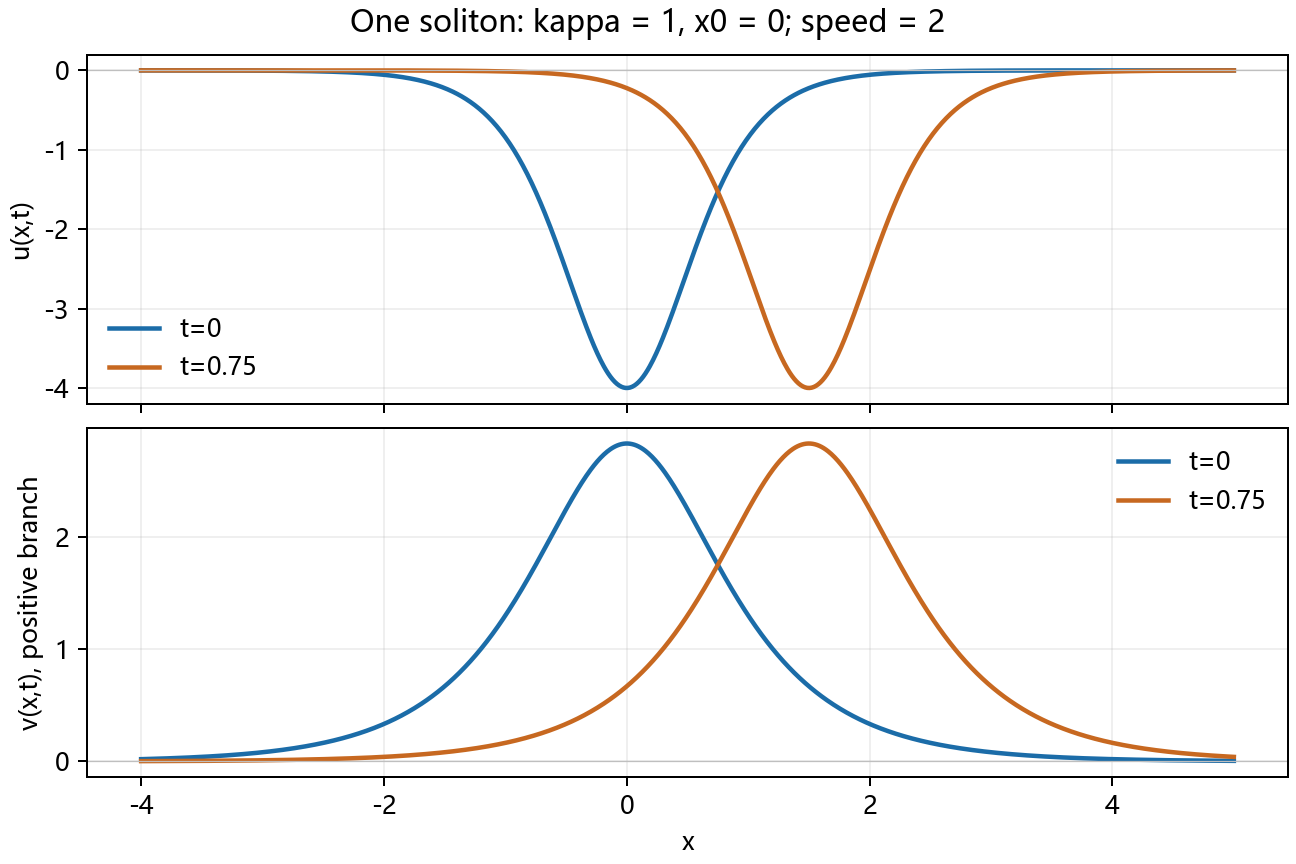
\includegraphics[width=0.94\textwidth]{figures/one-soliton.png}
\caption*{\textbf{Supplementary Figure S3.1／补充图 S3.1.} One soliton with $\kappa_1=1$, $x_0=0$ at two times.
同一个单孤子在 $t=0$ 与 $t=0.75$ 的两分量剖面；取 $v$ 的正号。中心由 0 移到 1.5，与速度 $2\kappa_1^2=2$ 一致。图由已核验的显式公式计算。}
\end{figure}

\appendix
\chapter{Tools and Reading Index／补充工具与阅读索引}
\section{Integral estimates／积分估计}
\begin{note}
本附录整理正文反复调用的最小工具；矩阵计算仍放在相应原文之后。没有增加八个区域的重复公式表。
\end{note}
\begin{lemma}[Volterra factorial estimate／Volterra 阶乘估计]
若 $q\geq0$ 可积，则对整数 $m\geq1$，
\[
\int_{-\infty}^xq(y_1)\int_{-\infty}^{y_1}q(y_2)\cdots
\int_{-\infty}^{y_{m-1}}q(y_m)\dd y_m\cdots\dd y_2\dd y_1
=\dfrac{1}{m!}\left(\int_{-\infty}^xq(y)\dd y\right)^m.
\]
\end{lemma}
\begin{proof}
Tonelli 定理允许把非负迭代积分看作区域 $y_m<\cdots<y_1<x$ 上的多重积分。
乘积 $\displaystyle \prod q(y_j)$ 对变量置换不变；除去两变量相等的零测度集合，整个直积区域 $(-\infty,x)^m$ 被 $m!$ 个排序区域不交分割。
各区积分相等，所以直积积分除以 $m!$ 即得所求。直积积分由 Tonelli 定理分离成 $m$ 个一维积分。
\end{proof}
\begin{lemma}[Integral Gronwall estimate／积分型 Gronwall 估计]
若 $h$ 有界非负，$q\geq0$ 可积，且 $\displaystyle h(x)\leq a+\int_{-\infty}^xq(y)h(y)\dd y$，$a\geq0$，则
$\displaystyle h(x)\leq a\exp(\int_{-\infty}^xq)$。特别地 $a=0$ 时 $h=0$。
\end{lemma}
\begin{proof}
把不等式右侧的 $h$ 反复代回。代回 $m$ 次后，常数项为
$a\displaystyle\sum\limits_{r=0}^{m-1}(\int_{-\infty}^xq)^r/r!$，末项至多 $\displaystyle \|h\|_\infty(\int_{-\infty}^xq)^m/m!$。
末项趋零，级数和为指数，结论成立。这也说明从负无穷开始的积分型估计需要可积控制与端点控制。
\end{proof}
\section{Analytic continuation and parameters／解析粘合与参数}
\begin{lemma}[Gluing across a ray／跨射线粘合]
一个函数在射线两侧解析、连续至射线，且两边界值相同，则在射线的非端点处有唯一解析延拓。
\end{lemma}
\begin{proof}
在跨射线的小圆盘内，沿射线把任意三角形截成有限多块，先将分割线平移到两侧，分别用 Cauchy 定理。由边界连续性取平移极限，内部边界的积分因反向相消，原三角形边界积分为零。
Morera 定理给出整个小圆盘解析性；恒等定理给出唯一性。逐元素应用即得矩阵版本。
\end{proof}
\begin{lemma}[Parameter analyticity／积分与级数的参数解析性]
若核对参数逐点解析，并在每个紧参数集上有与参数无关的可积控制函数，则积分解析。若解析级数在每个紧集上一致收敛，其和也解析。
\end{lemma}
\begin{proof}
对任意小三角形，Fubini 定理交换参数边界积分与空间积分；内部解析核的闭路积分为零，故由 Morera 定理解析。
级数情形由一致收敛交换闭路积分与求和，同理。连续到谱边界使用控制收敛定理；谱导数的控制函数应包含求导产生的所有空间矩，这正是反复要求 Schwartz 初值的原因。
\end{proof}
\section{Terminology and dependency index／术语与逻辑索引}
\begin{description}[style=nextline,leftmargin=1.5em]
\item[Lax 对（Lax pair）] §2.1；线性系统的相容性给出非线性 PDE。
\item[零曲率条件（zero-curvature condition）] §2.1；完整逐项计算及 $g_1,g_2$ 校勘。
\item[规范变换（gauge transformation）] $P$、(2.3)--(2.10)；对角化自由背景。
\item[Jost 解（Jost solution）] §2.2；从空间无穷端归一化。
\item[Volterra 积分方程（Volterra integral equation）] 命题 2.1、2.9；阶乘控制不要求位势小。
\item[散射矩阵（scattering matrix）] §2.3；合法域内的连接系数。
\item[伴随谱问题（adjoint spectral problem）] §2.4；负转置而非共轭转置。
\item[外幂及基本张量（exterior power; fundamental tensor）] §2.5；中间列通过整体张量解析延拓。
\item[加性扩张（additive extension）] 引理 2.2；生成元的和式，不能当作乘性外幂。
\item[广义叉积（generalized cross product）] 定义 2.2；将三阶张量变为四维列。
\item[基本亚纯解（fundamental meromorphic eigenfunction）] §2.6；逐分量混合端点归一化。
\item[Fredholm 行列式（Fredholm determinant）] 命题 2.10；异常点、亚纯性及可逆性。
\item[主子式（principal minor）] 定义 2.3；$S,T$ 分解的分母。
\item[反射系数（reflection coefficient）] 第 3 章、(3.1)；连续谱数据。
\item[跳跃条件（jump condition）] 引理 3.1、3.3；矩阵顺序与相位。
\item[谱奇点（spectral singularity）] 假设 3.1；射线上分母为零妨碍常规 RH 设定。
\item[留数条件（residue condition）] §3.2、(3.45)；特定纯孤子模型的附加条件。
\item[可去奇点（removable singularity）] 引理 3.6、3.7 及定理 3.3；分别处理原点与离散极点。
\item[重构公式（reconstruction formula）] 定理 3.2、3.3；无穷远系数恢复位势。
\item[范数常数（norming constant）] $\tau_j$、(3.44)；决定孤子位置及留数强度。
\end{description}
\section{A suggested reading route／建议阅读顺序}
\begin{enumerate}
\item 先读引言、§2.1 和定理 3.2，明确“初值—谱数据—时间相位—RH 解—位势”的闭环。
\item 再读 §2.2--2.4 的 Volterra、对称与渐近计算，注意每列、每个元素的合法定义域。
\item 集中读 §2.5 的加性扩张、二阶张量和叉积，解决中间列不能同时解析的障碍。
\item 读 §2.6 的 Fredholm 构造与 $S_1,T_1,S_8,T_8$ 消元；不需要背八套矩阵。
\item 读无孤子 RH 唯一性，自己复算留数矩阵乘积为零，以及 $1-c^4/k^4$ 的行列式。
\item 最后读纯孤子 RH 与二阶代数系统，独立代回两条 PDE。校勘随相应公式阅读。
\end{enumerate}

\backmatter
\chapter*{Acknowledgments／致谢}
\addcontentsline{toc}{chapter}{Acknowledgments／致谢}
\EN{This work was supported by the National Natural Science Foundation of China (Grant Nos. 12471234, 12171439) and Science Foundation of Henan Academy of Sciences (Grant No. 20252319002).}
\CN{本工作得到国家自然科学基金（项目号 12471234、12171439）及河南省科学院科学基金（项目号 20252319002）支持。}
\section*{Data Availability Statement／数据可用性声明}
\EN{Data sharing not applicable to this article as no data sets were generated or analyzed during the current study.}
\CN{本研究未生成或分析数据集，因此本文不适用数据共享声明。}
\chapter*{References／参考文献}
\addcontentsline{toc}{chapter}{References／参考文献}
\begin{note}
以下保留原文 33 个参考文献序号及著录，题名附中文译名。外部文献的历史结论按原作者引用理解，未核读的文献不作为本笔记独立验证的来源。
原文 [1]、[2] 的作者名印为 Hirita，[3] 印为 Green，照录保留；常见规范拼写分别为 Hirota、Greene。
本文期刊原件：H. Zhang, X. Geng, H. Liu, \emph{Studies in Applied Mathematics} 155 (2025), e70113，\href{https://doi.org/10.1111/sapm.70113}{doi:10.1111/sapm.70113}。
\end{note}
\begin{enumerate}[label={[\arabic*]},leftmargin=2.8em]
\item R. Hirita and J. Satsuma, ``Soliton Solutions of a Coupled Korteweg-de Vries Equation,'' \emph{Physics Letters A} 85 (1981): 407--408.
\CN{耦合 Korteweg--de Vries 方程的孤子解。}
\item R. Hirita and J. Satsuma, ``A Coupled KdV Equation is One Case of the Four-Reduction of the KP Hierarchy,'' \emph{Journal of the Physical Society of Japan} 51 (1982): 3390--3397.
\CN{一种耦合 KdV 方程是 KP 层级四约化的一个特例。}
\item C. S. Gardner, J. M. Green, M. D. Kruskal, and R. M. Miura, ``Method for Solving the Korteweg--de Vries Equation,'' \emph{Physical Review Letters} 19 (1967): 1095--1097.
\CN{求解 Korteweg--de Vries 方程的方法。}
\item K. Grunert and G. Teschl, ``Long-Time Asymptotics for the Korteweg--de Vries Equation via Nonlinear Steepest Descent,'' \emph{Mathematical Physics, Analysis and Geometry} 12 (2009): 287--324.
\CN{通过非线性最速下降法研究 KdV 方程的长时间渐近行为。}
\item R. Dodd and A. P. Fordy, ``On the Integrability of a System of a Coupled KdV Equation,'' \emph{Physics Letters A} 89 (1982): 168--170.
\CN{论一个耦合 KdV 方程组的可积性。}
\item W. H. Tam, W. X. Ma, X. B. Hu, and D. L. Wang, ``The Hirota--Satsuma Coupled KdV Equation and a Coupled Ito System Revisited,'' \emph{Journal of the Physical Society of Japan} 69 (2000): 45--52.
\CN{再论 Hirota--Satsuma 耦合 KdV 方程与耦合 Ito 系统。}
\item D. Levi, ``A Hierarchy of Coupled Korteweg--de Vries Equation,'' \emph{Physics Letters A} 95 (1983): 7--10.
\CN{一个耦合 KdV 方程层级。}
\item H. C. Hu and Q. P. Liu, ``New Darboux Transformation for Hirota--Satsuma Coupled KdV System,'' \emph{Chaos, Solitons \& Fractals} 17 (2003): 921--928.
\CN{Hirota--Satsuma 耦合 KdV 系统的新 Darboux 变换。}
\item\phantomsection\label{ref:original9} Y. T. Wu, X. G. Geng, X. B. Hu, and S. M. Zhu, ``A Generalized Hirota--Satsuma Coupled Korteweg--de Vries Equation and Miura Transformations,'' \emph{Physics Letters A} 255 (1999): 259--264.
\CN{广义 Hirota--Satsuma 耦合 KdV 方程及 Miura 变换。}
\item X. Zhou, ``The Riemann-Hilbert Problem and Inverse Scattering,'' \emph{SIAM Journal on Mathematical Analysis} 20 (1989): 966--986.
\CN{Riemann--Hilbert 问题与逆散射。}
\item P. Deift and X. Zhou, ``A Steepest Descent Method for Oscillatory Riemann--Hilbert Problems. Asymptotics for the MKdV Equation,'' \emph{Annals of Mathematics} 137 (1993): 295--368.
\CN{振荡 RH 问题的最速下降法及 mKdV 方程的渐近行为。}
\item X. G. Geng and H. Liu, ``The Nonlinear Steepest Descent Method to Long-Time Asymptotics of the Coupled Nonlinear Schrödinger Equation,'' \emph{Journal of Nonlinear Science} 28 (2018): 739--763.
\CN{耦合非线性薛定谔方程长时间渐近的非线性最速下降法。}
\item X. G. Geng, K. D. Wang, and M. M. Chen, ``Long-Time Asymptotics for the Spin-1 Gross--Pitaevskii Equation,'' \emph{Communications in Mathematical Physics} 382 (2021): 585--611.
\CN{自旋为一的 Gross--Pitaevskii 方程的长时间渐近。}
\item X. G. Geng, J. Wang, K. D. Wang, and R. M. Li, ``Soliton Resolution for the Complex Short-Pulse Positive Flow With Weighted Sobolev Initial Data in the Space-Time Soliton Regions,'' \emph{Journal of Differential Equations} 386 (2024): 214--268.
\CN{加权 Sobolev 初值的复短脉冲正流在时空孤子区中的孤子分解。}
\item R. Beals and R. R. Coifman, ``Scattering and Inverse Scattering for First Order Systems,'' \emph{Communications on Pure and Applied Mathematics} 37 (1984): 39--90.
\CN{一阶系统的散射与逆散射。}
\item R. Beals, P. Deift, and C. Tomei, \emph{Direct and Inverse Scattering on the Line} (American Mathematical Society, 1988).
\CN{直线上的正散射与逆散射。}
\item B. Prinari, G. Biondini, and A. D. Trubatch, ``Inverse Scattering Transform for the Multi-Component Nonlinear Schrödinger Equation With Nonzero Boundary Conditions,'' \emph{Studies in Applied Mathematics} 126 (2011): 245--302.
\CN{非零边界条件下多分量非线性薛定谔方程的逆散射变换。}
\item G. Biondini, D. Kraus, and B. Prinari, ``The Three-Component Defocusing Nonlinear Schrödinger Equation With Nonzero Boundary Conditions,'' \emph{Communications in Mathematical Physics} 348 (2016): 475--533.
\CN{非零边界条件下三分量散焦非线性薛定谔方程。}
\item A. B. de Monvel and D. Shepelsky, ``A Riemann-Hilbert Approach for the Degasperis-Procesi Equation,'' \emph{Nonlinearity} 26 (2013): 2081--2107.
\CN{Degasperis--Procesi 方程的 RH 方法。}
\item A. B. de Monvel, D. Shepelsky, and L. Zielinski, ``A Riemann--Hilbert Approach for the Novikov Equation,'' \emph{Symmetry, Integrability and Geometry: Methods and Applications} 12 (2016): 1--22.
\CN{Novikov 方程的 RH 方法。}
\item A. B. de Monvel and D. Shepelsky, ``The Ostrovsky-Vakhnenko Equation by a Riemann-Hilbert Approach,'' \emph{Journal of Physics A} 48 (2015): 035204.
\CN{用 RH 方法研究 Ostrovsky--Vakhnenko 方程。}
\item C. Charlier and J. Lenells, ``The `Good' Boussinesq Equation: A Riemann--Hilbert Approach,'' \emph{Indiana University Mathematics Journal} 71 (2022): 1505--1562.
\CN{良性 Boussinesq 方程的 RH 方法。}
\item C. Charlier, J. Lenells, and D. S. Wang, ``The `Good' Boussinesq Equation: Long-Time Asymptotics,'' \emph{Analysis \& PDE} 6 (2023): 1351--1388.
\CN{良性 Boussinesq 方程的长时间渐近。卷号按原文照录。}
\item C. Charlier and J. Lenells, ``On Boussinesq's Equation for Water Waves,'' preprint, 2023, doi:10.48550/arXiv.2204.02365 [nlin.SI].
\CN{论水波的 Boussinesq 方程。}
\item D. S. Wang and X. D. Zhu, ``Long-Time Asymptotics of the Sawada-Kotera Equation and Kaup-Kupershmidt Equation on the Line,'' preprint, 2023, doi:10.48550/arXiv.2307.08196 [nlin.SI].
\CN{直线上 Sawada--Kotera 与 Kaup--Kupershmidt 方程的长时间渐近。}
\item D. S. Wang, C. Zhu, and X. D. Zhu, ``Miura Transformations and Large-Time Behaviors of the Hirota-Satsuma Equation,'' preprint, 2024, doi:10.48550/arXiv.2404.01215 [nlin.SI].
\CN{Hirota--Satsuma 方程的 Miura 变换与大时间行为。原文 DOI 域名中的排印点号在此改正。}
\item L. Huang, D. S. Wang, and X. D. Zhu, ``Long-Time Asymptotics of the Tzitzéica Equation on the Line,'' preprint, 2024, doi:10.48550/arXiv.2404.04999 [nlin.SI].
\CN{直线上 Tzitzéica 方程的长时间渐近。}
\item P. J. Caudrey, ``The Inverse Problem for the Third Order Equation $u_{xxx}+q(x)u_x+r(x)u=-\ii\zeta^3u$,'' \emph{Physics Letters A} 79 (1980): 1819--1826.
\CN{三阶谱方程的逆问题。}
\item P. Deift and C. Tomei, ``Inverse Scattering and the Boussinesq Equation,'' \emph{Communications on Pure and Applied Mathematics} 35 (1982): 567--628.
\CN{逆散射与 Boussinesq 方程。}
\item L. Huang and J. Lenells, ``Nonlinear Fourier Transforms for the Sine-Gordon Equation in the Quarter Plane,'' \emph{Journal of Differential Equations} 264 (2018): 3445--3499.
\CN{四分之一平面上 sine--Gordon 方程的非线性 Fourier 变换。}
\item H. Liu, J. Shen, and X. G. Geng, ``Inverse Scattering Transformation for the N-Component Focusing Nonlinear Schrödinger Equation With Nonzero Boundary Conditions,'' \emph{Letters in Mathematical Physics} 113 (2023): 1--47.
\CN{非零边界条件下 N 分量聚焦非线性薛定谔方程的逆散射变换。}
\item P. J. Caudrey, ``The Inverse Problem for a General $N\times N$ Spectral Equation,'' \emph{Physica D} 6 (1982): 51--66.
\CN{一般 N 阶矩阵谱方程的逆问题。}
\item V. E. Zakharov and A. B. Shabat, ``A Plan for Integrating the Nonlinear Equations of Mathematical Physics by the Method of the Inverse Scattering Problem. I,'' \emph{Functional Analysis and Its Applications} 8 (1974): 226--235.
\CN{用逆散射问题方法积分数学物理非线性方程的方案，第一部分。}
\end{enumerate}
\section*{Additional background／补充先修资料}
范恩贵：《可积系统、正交多项式和随机矩阵——Riemann--Hilbert 方法》，仓库中的二校版（文件日期标识 20220303）。以其前六章作为阅读背景；新用到的外幂与 Fredholm 构造在正文实际使用处解释。
\section*{Publication notice／原件出版说明}
\EN{\copyright\ 2025 Wiley Periodicals LLC.}
\CN{原件出版版权：2025 年 Wiley Periodicals LLC。}
\EN{Copyright of Studies in Applied Mathematics is the property of Wiley-Blackwell and its content may not be copied or emailed to multiple sites or posted to a listserv without the copyright holder's express written permission. However, users may print, download, or email articles for individual use.}
\CN{原件附页说明：《Studies in Applied Mathematics》的版权属于 Wiley--Blackwell；未经版权人明确书面许可，其内容不得复制或群发至多个站点或邮件列表。用户可以为个人使用打印、下载或发送文章。}

\end{document}
